% !TeX program = lualatex
% !TeX root = luaking.tex
% !TeX encoding = UTF-8
% !TeX spellcheck = cs_CZ
%---------------------------------------------------------------------------------------------------
% file fey1ch01_02_03.tex
\graphicspath{{../src/FYZ/img/}}
%---------------------------------------------------------------------------------------------------
%================ Kapitola: Elektromagnetizmus======================================================
\setchaptertoc
\chapter{Elektromagnetizmus}\label{fyz:IIchapI}
  \section{Elektrické síly}\label{fyz:IIchapIsecI}
    \cite[s.~13]{Feynman02} Představme si sílu, která se podobá gravitaci a mění se převážně nepřímo
    úměrně druhé mocnině vzdálenosti, ale asi miliardu miliard miliard miliard-krát větší. A ještě 
    s jedním rozdílem. Nechť existují dva druhy „látky“, nazývejme je kladná a záporná. Nechť na 
    rozdíl od gravitace, v níž existuje pouze přitahování, se stejné druhy odpuzují a odlišné druhy 
    přitahují. Co by se stalo?
    
    Chomáč kladné látky by se ohromnou silou odpuzoval a rozptýlil by se na všechny strany. S
    chomáčem záporné by se stalo totéž. Ale směs stejného množství kladné a záporné látky by se
    chovala zcela odlišně. Ohromná přitažlivá síla by přitáhla opačné kousky k sobě. V konečném
    důsledku by se tyto úžasné síly navzájem téměř dokonale vykompenzovaly vytvořením hutných
    jemných směsí kladného a záporného, přičemž mezi dvěma oddělenými chomáči takových směsí by
    neexistovalo téměř žádné přitahování nebo odpuzování.
    
    \luagraphic[0.9]{fyz_fig0145.jpg}{Empire State Building, 1934}{fyz:fig0145} 
    Taková síla existuje - je to \emph{elektrická síla}! A každá látka je směsí kladných protonů a 
    záporných elektronů, které se touto velkou silou přitahují a odpuzují. Ale vyvážení je tak 
    dokonalé, že když stojíte blízko někoho jiného, necítíte sílu vůbec žádnou. Kdyby existoval jen 
    malý zbytek nerovnováhy, poznali bychom to. Kdybyste stáli od někoho na vzdálenost paže a každý 
    z vás by měl o jedno procento víc elektronů než protonů, byla by odpudivá síla mezi vámi 
    neuvěřitelná. Jak velká? Dost na to, aby zvedla obrovský mrakodrap? Ne! Aby zvedla Mount 
    Everest? Ne! Odpuzování by stačilo na zvednutí břemene s hmotností celé zeměkoule!

    S ohledem na tak perfektní vyvážení ohromné síly, působící v této směsi, není těžké pochopit, že
    látka s tendencí udržet své kladné a záporné náboje v nejjemnější rovnováze může mít velkou
    tvrdost a pevnost. Mrakodrap \wikiELB (obr. \ref{fyz:fig0145}) se například vychyluje ve větru
    jen o necelé tři metry, neboť elektrické síly udržují každý elektron a proton víceméně ve stálé
    poloze. Na druhé straně, když se podíváme na tak malé množství látky, že uvidíme jen několik
    atomů, libovolná malá část látky obvykle nebude mít stejný počet kladných a záporných; nábojů,
    takže budou existovat velké zbytkové elektrické síly. I kdyby byly počty obou druhů nábojů ve
    dvou sousedních malých částech stejné, pravděpodobně ještě zůstanou mezi oběma částmi elektrické
    síly, neboť síly mezi jednotlivými náboji se mění nepřímo úměrně s druhou mocninou vzdálenosti.
    Zbytková síla může vzniknout, nachází-li se záporný náboj jedné části blíž kladnému náboji než
    kladný náboj zápornému v části jiné. Pak mohou být přitažlivé síly větší než odpudivé a může
    dojít k výslednému přitahování i dvou částí bez nadbytečných nábojů. Síla, která \uv{udržuje}
    pohromadě atomy, a chemická síla, která drží molekuly, jsou ve skutečnosti elektrickými silami
    působícími v oblastech s nedokonalou rovnováhou nábojů anebo s velmi malými vzdálenostmi.

    Samozřejmě víme, že se atomy skládají z kladných protonů v jádře a záporných elektronů v jeho 
    okolí. Můžeme se ptát: Když je tato elektrická síla tak úžasná, proč spolu protony a elektrony 
    nesplynou? Když mají tvořit dokonalou směs, proč tato směs není ještě dokonalejší? Odpověď 
    nacházíme v kvantových jevech. Pokusíme-li se naše elektrony uzavřít do oblasti těsně 
    přiléhající k protonům, musí mít podle principu neurčitosti nenulovou střední kvadratickou 
    hybnost, která je tím větší, čím těsnější je ohraničení. Právě tento pohyb, vyplývající ze 
    zákonů kvantové mechaniky, zabraňuje elektrické přitažlivosti dostat náboje jakýmkoli způsobem 
    blíž k sobě.
    
    Je tu další otázka: Co drží pohromadě atomové jádro? V jádře je několik kladných protonů. Proč 
    se od sebe neoddělí? Ukazuje se, že v jádře existují kromě elektrických i neelektrické síly, 
    které se nazývají jaderné síly. Jsou větší než elektrické síly a jsou schopné držet protony u 
    sebe i přes jejich elektrické odpuzování. Síly jádra však mají malý dosah - jejich velikost 
    klesá mnohem rychleji než \(\frac{1}{r^2}\). A to má důležitý důsledek. Kdyby jádro obsahovalo 
    velmi mnoho protonů, stalo by se příliš velkým a nezůstalo by pohromadě. Příkladem je uran s 
    \(92\) protony. Jaderné síly působí převážně jen mezi každým protonem (nebo neutronem) a jeho 
    nejbližším sousedem, ale elektrické síly působí i na větší vzdálenosti a vyvolávají tak 
    odpuzování každého protonu od všech ostatních v jádře. Čím víc je v jádře protonů, tím je 
    elektrické odpuzování silnější, až dokud - jako v případě uranu - není rovnováha tak křehká, že 
    je jádro účinkem elektrické síly téměř připraveno se rozletět. Jestliže takové jádro jen trochu 
    „postrčíme“ (pokud do něj vyšleme pomalý neutron), rozdělí se na dvě části s kladným nábojem. V 
    důsledku elektrického odpuzování od sebe obě části odletí. Energie, která se při tom 
    uvolňuje, je energií atomové bomby. Obvykle se tato energie nazývá jaderná, ale v podstatě je 
    to elektrická energie uvolněná tehdy, když elektrické síly překonaly přitažlivé síly jádra.
    
    Konečně se můžeme ptát, co drží pohromadě záporný elektron (neboť ten nemá žádné jaderné síly). 
    Skládá-li se elektron celý z jednoho druhu látky, každá z jeho částí by měla odpuzovat ty 
    ostatní. Proč se tedy nerozletí? Má však elektron „části“? Asi bychom měli říct, že elektron je 
    jen bod a že elektrické síly působí jen mezi různými dvěma bodovými náboji, takže sám na sebe 
    elektron nepůsobí. Snad. Vše, co můžeme říct, je, že otázka, co drží pohromadě elektron, 
    způsobila v pokusech o vytvoření úplné teorie elektromagnetizmu mnoho těžkostí. Tato otázka 
    zatím nebyla zodpovězena. V dalších kapitolách se budeme tomuto tématu věnovat více.
    
    Jak jsme viděli, je třeba čekat, že právě kombinace elektrických sil a kvantově mechanických 
    jevů bude určovat detailní strukturu makroskopických množství látek, a tím i jejich vlastnosti. 
    Některé látky jsou tvrdé, jiné měkké. Některé jsou elektrickými vodiči, protože jejich 
    elektrony se mohou volně pohybovat, jiné jsou izolátory, protože jejich elektrony jsou pevné 
    připoutané k jednotlivým atomům. Později budeme hovořit o tom, jak vznikají některé z těchto 
    vlastností. Je to však složitá otázka, proto nejdřív budeme zkoumat elektrické síly jen v 
    jednoduchých situacích. Začněme s probíráním zákonů elektřiny, včetně magnetizmu, který je 
    vlastně částí téhož předmětu.

    O přítomnosti elektrického náboje se tedy přesvědčujeme pouze na základě jeho silového projevu.
    Znamená to, že existenci jednoho jediného náboje bychom nemohli nijak odhalit. Kdyby
    existovaly pouze dva náboje, mohli bychom určit, zda jsou souhlasného či nesouhlasného
    znamení, nemohli bychom však rozhodnout ani o znamení, ani o velikosti těchto nábojů. Teprve
    jsou-li k dispozici alespoň tři náboje, můžeme jeden z nich vybrat jako jednotkový a kladný a
    ze silového působení určit velikost a znamení druhých nábojů. Tato síla podobně jako gravitační 
    klesá nepřímo úměrně s druhou mocninou vzdálenosti mezi náboji. Tento vztah se nazývá 
    \hyperlink{fyz:IIchapIVsecII}{Coulombův zákon}. Ale neplatí přesně, když se náboje pohybují, 
    protože elektrické síly závisí také na pohybu nábojů, a to komplikovaným způsobem. Jednu část 
    síly mezi pohybujícími se náboji nazýváme \emph{magnetická síla}, která vlastně představuje 
    jeden aspekt elektrického účinku. Právě proto hovoříme o „elektromagnetizmu“.
    
    Existuje důležitý obecný princip, který umožňuje zacházet s elektromagnetickými silami poměrně 
    snadno. Experimentálně se zjistilo, že síla působící na náboj závisí pouze na poloze tohoto 
    náboje, jeho rychlosti a velikosti, bez ohledu na to, kolik dalších nábojů existuje a jak se 
    pohybují. Sílu \(\vec{F}\) působící na náboj \(q\), který se pohybuje rychlostí \(\vec{v}\), 
    můžeme vyjádřit takto:
    \begin{equation}\label{fyz:eq_fey_elmag01}
      \boxed{\vec{F} = q(\vec{E}+\vec{v}\times\vec{B})}\, ,
    \end{equation}
    kde \(\vec{E}\) je \emph{elektrické pole} a \(\vec{B}\) \emph{magnetické pole} v místě, kde se 
    nachází náboj. Důležité je, že elektrické síly všech nábojů ve vesmíru lze složit právě z 
    těchto dvou vektorů. Jejich hodnoty závisí na tom, kde se uvažovaný náboj nachází, a mohou se v 
    čase měnit. Kromě toho, nahradíme-li tento náboj jiným, změní se síla působící na nový náboj v 
    poměru velikostí obou nábojů, nezmění-li všechny ostatní náboje na světě svou polohu nebo 
    pohyb. (Samozřejmě že v reálné situaci každý náboj působí na všechny ostatní ve svém okolí a 
    může je uvést do pohybu. A tak když v některých případech nahradíme náš určitý náboj jiným 
    nábojem, mohou se pole změnit.)
    
    Z \ref{vol02:part:FYZI}. dílu víme, jak se určuje pohyb částice, známe-li sílu, která na ni
    působí. Dosadíme-li výraz (\ref{fyz:eq_fey_elmag01}) do pohybové rovnice, dostaneme
    \begin{equation}\label{fyz:eq_fey_elmag02}
      \der{ }{t}\left(\frac{m\vec{v}}{\sqrt{1-\frac{v^2}{c^2}}}\right) = \vec{F} =
      q(\vec{E}+\vec{v}\times\vec{B})
    \end{equation}
    Známe-li \(\vec{E}\) a \(\vec{B}\), můžeme určit pohyby nabitých částic. K tomu už jen 
    potřebujeme vědět, jak \(\vec{E}\) a \(\vec{B}\) vznikají.
    
    Jeden z nejdůležitějších zjednodušujících principů vytváření elektrických polí závisí na tomto:
    Předpokládejme, že určitý počet nábojů pohybujících se libovolným způsobem vytvoří pole 
    \(\vec{E_1}\) a jiná množina nábojů vytvoří pole \(\vec{E_2}\). Působí-li obě množiny nábojů 
    současně (při zachování stejných pohybů a poloh, které měly, když jsme o nich uvažovali 
    odděleně), vytvoří pole, které je dáno součtem
    \begin{equation}\label{fyz:eq_fey_elmag03}
      \vec{E} = \vec{E_1} + \vec{E_2}
    \end{equation}
    Tento fakt se nazývá princip \emph{superpozice polí}. Platí také pro magnetická pole.
    
    Z tohoto principu vyplývá, že budeme-li vědět, podle jakého zákona vytváří elektrická a
    magnetická pole jediný náboj pohybující se libovolným způsobem, zákony elektrodynamiky už budou
    úplné. Chceme-li znát sílu působící na náboj \(A\), je třeba spočítat pouze \(\vec{E}\) a
    \(\vec{B}\), které vytváří každý náboj \(B\), \(C\), \(D\) atd., pak vypočítat vektory
    \(\vec{E}\) a \(\vec{B}\) všech nábojů, a tak najít  pole a síly působící z nich na \(A\). Kdyby
    se ukázalo, že zákon, podle kterého se vytváří pole jediného náboje, je jednoduchý, byla by to
    nejšikovnější cesta, jak popsat zákony elektrodynamiky. My už jsme uvedli tento zákon (kapitola
    \ref{vol02:fyz:IchapXXVIII}, díl \ref{vol02:part:FYZI}), který je, bohužel, dost složitý.
    
    Ukazuje se, že tvar, ve kterém jsou zákony elektrodynamiky nejednodušší, není tím tvarem, který 
    bychom zde mohli očekávat. Není totiž vůbec jednoduché udat vzorec síly, kterou působí jeden 
    náboj na druhý. Je pravda, že pokud jsou náboje v klidu, je výraz pro Coulombovu sílu ještě 
    jednoduchý, ale když se náboje pohybují, vztahy se komplikují kromě jiného i časovým zpožděním 
    a zrychlením. Z tohoto důvodu nehodláme prezentovat elektrodynamiku pouze prostřednictvím 
    zákonů síly působící mezi náboji; pokládáme za vhodnější jiné hledisko - při něm jsou zákony 
    elektrodynamiky zvládnutelné snáze.

    \subsection{Elektrický náboj}\label{fyz:IIchapIsecII} 
      Jak už bylo řečeno v kapitole \ref{fyz:IIchapI} o elektřině víme, že některá tělesa (například
      skleněná či ebonitová tyč po předchozím tření) mohou za určitých podmínek silově působit na
      jiná tělesa. Toto silové působení si vysvětlujeme přítomností elektrických nábojů.

      \fbox{Elektrický náboj} představuje pro nás výchozí fyzikální veličinu, přičemž mírou jejího
      množství a rozložení na příslušných tělesech je právě silové působení mezi nimi. Elektrický
      náboj je veličinou \textbf{skalární}, podobně jako hmotnost, a k jeho určení postačí jediná
      (reálná) číselná hodnota. Jednotkou je \emph{coulomb [C]}. Má kvantový charakter (tj. je roven
      celistvému násobku elementárního náboje $e = 1,602\cdot10^{-19}C$), avšak v technických
      aplikacích k tomu nepřihlížíme. Náboj $Q$ může být rozložen:
      \begin{itemize}[noitemsep]
        \item \emph{prostorově} v objemu $V$ s objemovou hustotou
            \begin{equation}\label{TEMP:eq_q_varrho}
              \varrho = \frac{dQ}{dV} \quad [C\cdot m^{-3}]
            \end{equation}               
        \item \emph{plošně} na ploše $S$, s plošnou hustotou
            \begin{equation}\label{TEMP:eq_q_sigma}
              \sigma = \frac{dQ}{dS} \quad [C\cdot m^{-2}]
            \end{equation}                 
        \item \emph{lineárně} na křivce $l$, s lineární hustotou
            \begin{equation}\label{TEMP:eq_q_tau}
              \tau = \frac{dQ}{dl} \quad [C\cdot m^{-1}]
            \end{equation}                 
      \end{itemize}
      Rozlišujeme:
        \begin{itemize}[noitemsep]
          \item \textbf{volné náboje}: mohou se přemisťovat v makroskopických vzdálenostech,
          \item \textbf{vázané náboje}: mohou se přemisťovat jen v mikroskopických vzdálenostech.
        \end{itemize}
      Volnými náboji jsou volné elektrony v kovech nebo ionty v elektrolytech (jsou odpoutány od
      atomů, resp. molekul a volně se mezi nimi pohybují); vázané náboje vznikají polarizací
      dielektrika.    
      
      Skutečnost, že síly elektrického působení mezi tělesy mohou být jak přitažlivé, tak odpudivé,
      vysvětlujeme tím, že elektrický náboj může nabývat \emph{kladných} i \emph{záporných} hodnot -
      tělesa se souhlasným znamením náboje se přitom odpuzují, tělesa s nesouhlasným znamením náboje
      se přitahují. Tělesa, která nesou elektrický náboj, nazýváme kladně či záporně nabitá, tělesa
      o nulovém náboji jsou elektricky neutrální, nenabitá. Často se setkáváme s případem, kdy na
      tělesech jsou odděleně rozloženy kladné a záporné elektrické náboje o téže absolutní hodnotě.
      Taková tělesa budou také elektricky silově působit, přestože jejich celkový elektrický náboj
      je nulový. Říkáme jim \emph{polarizovaná}. 
      
      O přítomnosti elektrického náboje se přesvědčujeme \emph{pouze} na základě jeho
      \textbf{silového působení}. Znamená to, že existenci jednoho jediného náboje bychom nemohli
      nijak odhalit. Kdyby existovaly pouze dva náboje, mohli bychom určit, zda jsou souhlasného či
      nesouhlasného znamení; nemohli bychom však rozhodnout ani o znamení, ani o velikosti těchto
      nábojů. Teprve jsou-li k dispozici alespoň tři náboje, můžeme jeden z nich vybrat jako
      jednotkový a kladný a ze silového působení určit velikost a znamení druhých dvou nábojů
      (\cite[s.~15]{Stoll2012}).
      
      V denním životě se setkáváme s projevy působení gravitačního a elektromagnetického, které je
      ze všech nejlépe prozkoumáno. Nejen elektrostatické a elektrodynamické, ale i magnetické,
      optické, chemické a biologické jevy, chemické vazby a uvolňování chemické energie,
      mezimolekulární sily podmiňující soudržnost těles, přilnavost a tření, síly svalové kontrakce,
      tepelné působení slunečního záření a mnoho dalších jevů má svůj původ ve vzájemném působení
      elektrických nábojů.
      
      Síly elektromagnetického působení mohou být přitažlivé i odpudivé, mohou složitým způsobem
      záviset na vzdálenosti, směru v prostoru a vzájemné poloze těles, na rychlosti jejich pohybu,
      vlastnostech prostředí, obecně nemusí působit ve směru spojnice interagujících těles, a
      dokonce nemusí ani splňovat Newtonův zákon akce a reakce.
      
      Elektrický náboj má některé základní vlastnosti, které vyplývají z experimentálních pozorování
      a uplatňují se i při vzájemné interakci nabitých částic. Tyto vlastností vyjadřuje:    
      \begin{description}[leftmargin=2em,labelindent=1em, style=nextline]
        \item[Zákon zachování náboje] Elektrický náboj je nestvořitelný a nezničitelný. Jinak
              řečeno, celkové množství elektrického náboje v elektricky izolované soustavě (jejíž
              hranicí nemohou procházet náboje) zůstává neměnné. Docházi-li ke srážkám částic, je
              celkový náboj před reakcí roven celkovému náboji po reakci. První experimentální důkaz
              tohoto zákona podal Faraday v r. 1843 elektrometrickým měřením náboje nabité koule v
              izolovaném prostoru. Matematické vyjádření tohoto zákona je dáno tzv. \emph{rovnicí
              kontinuity proudu}, kterou uvedeme v článku ***. %3.1.3. 
        \item[Zákon invariantnosti náboje] Velikost elektrického náboje se při pohybu nemění. Jinak
              řečeno, při všech transformacích vztažné soustavy Zůstává velikost náboje invariantní.
              Takovou vlastnost má jen málo fyzikálních veličin: například hmotnost částice roste
              jak známo s rychlostí.
        \item[Zákon kvantování náboje] Existuje nejmenší, dále nedělitelný elektrický náboj, který
              nazýváme elementárním, a všechny elektrické náboje mají velikost, která je jeho
              celistvým násobkem. Tento atomismus elektřiny souvisí s tím, že elektrický náboj je
              vlastností částic látky. Velikost elementárního náboje je možné určit pomocí celé řady
              experimentů, např. klasického Millikanova pokusu (1911), viz článek ***. % 1.1.3
      \end{description}

      Pokud jde o vlastnosti nabitých částic, jsou pozoruhodné ještě dvě okolnosti. Jednou z nich je
      existence \emph{částic a antičástic}. Ke každé částici existuje antičástice, které se vzájemně
      liší znamením elektrického náboje\footnote{Částice a antičástice se liší též znaménkem
      magnetického momentu a některých dalších tzv. \emph{kvantových čísel} (leptonový a  baryonový
      náboj, podivnost, půvab aj.), která charakterizují jejich vzájemné interakce. Existuje několik
      částic, které jsou se svými antičásticemi totožné (například foton)}. Protože elektrické síly
      závisejí pouze na souhlasnosti či nesouhlasnosti znamení náboje, mohla by existovat antilátka,
      kde by nukleony v atomových jádrech byly nahrazeny antinukleony a elektrony atomových obalů
      svými antičásticemi - pozitrony. Tyto úvahy mají velký význam i pro kosmologii a vyjadřují
      jednu ze základních symetrií přírody.
      
      Druhá ze zmíněných okolností je \emph{nábojová kvazineutralita} vesmíru. V dostatečně velkých
      objemech se celkový počet kladných i záporných nábojů vždy vyrovnává a látka, jak se s ní
      běžně setkáváme v tuhém, kapalném a plynném skupenství, se jeví elektricky neutrální. Odchylky
      od elektrické neutrality v makroskopických měřítcích se projevují elektrickými silami, které
      se opět snaží elektrickou neutralitu obnovit.

      \begin{tcnote}
        Co je vlastní podstatou elektrického náboje nevíme. Na základě poznatků o mikrosvětě (rok
        2000) jej můžeme považovat za jednu z vlastností elementárních částic, která podmiňuje
        jejich vzájemné působení. Rozlišujeme čtyři základní typy vzájemného působení
        (\emph{interakce}) mezi elementárními částicemi: \emph{gravitační, slabé, elektromagnetické
        a silné}. Gravitační interakce je univerzální a týká se všech částic. Setkali jsme se s ní v
        mechanice, její velikost udává Newtonův gravitační zákon a její podstatu se snaží objasnit
        obecná teorie relativity. Slabá interakce se projevuje u některých typů radioaktivního
        rozpadu za účasti neutrina. Podobně elektromagnetická interakce se uplatňuje mezi
        elementárními částicemi a jednou z jejích charakteristik je náboj. Silná interakce existuje
        mezi částicemi, které nazýváme hadrony, a drží pohromadě atomové jádro, které by se jinak
        odpudivými elektrickými silami působícími mezi protony musely rozdělit.
        
        Současný rozvoj mikrofyziky naznačuje, že hadrony, které jsme dříve považovali za
        elementární, mají svoji strukturu a komponenty. Předpokládáme o nich, že jsou tvořeny tzv.
        kvarky. Na současné úrovni vystupují tedy jako elementární kvarky a leptony (k nim patří
        elektron, mion, tauon a odpovídající neutrina), jejich antičástice a dále pak částice, které
        zprostředkovávají interakci mezi nimi.
      \end{tcnote}

      % --------example: Velikost náboje v minci -----------------------
      % \label{fyz:exam035}
      % !TeX spellcheck = cs_CZ
%---------- Velikost náboje v minci:
\begin{fyzexam}{Velikost náboje v minci}{exam035}
  Elektricky neutrální měděná mince o hmotnosti \(m = \qty{3.11}{\g}\) obsahuje stejné množství
  kladného a záporného náboje. Jaké je velikost kladného (nebo záporného) náboje obsaženého v
  minci?

\tcbsubtitle[before skip=\baselineskip]{Řešení:} 
  Neutrální atom má záporný náboj \(Z\cdot e\), představovaný jeho elektrony a kladný náboj o stejné
  velikosti představovaný protony v jádře. Pro měď je atomové číslo \(Z\) rovno \num{29}, tj. atom
  mědi má \num{29} protonů, a je-li elektricky neutrální, také \num{29} elektronů.
  
  Náboj o velikosti \(Q_v\), který hledáme je roven \(N\cdot Z\cdot e\), kde \(N\) je počet atomů
  obsažených v  jednom molu (Avogadrova konstanta: \(N_A = \qty{6.0221e23}{\per\mole}\)). Počet molů
  mědi v minci \(\frac{m}{M}\), kde \(M = \qty{63.5}{\g\per\mole}\) je molární hmotnosti mědi:    
  \begin{align*}
    N &=N_A\cdot\frac{m}{M}
       =\qty{6.0221e23}{\per\mole}\frac{\qty{3.11}{\g}}{\qty{63.5}{\g\per\mole}}    \\ 
      &=\num{2.95e22}.
  \end{align*}
  Velikost celkového kladného (záporného) náboje v minci je pak 
  \begin{align*}
    Q_v &= N\cdot Z\cdot e = \num{2.95e22}\cdot\num{29}\cdot\qty{1.602e-19}{\coulomb}    \\
        &= \qty{137039}{\coulomb}
  \end{align*}
  To je obrovský náboj. Pro srovnání: třeme-li ebonitovou tyč vlněnou látkou, můžeme na tyč
  přemístit stěží náboj o velikosti \qty{1e-9}{\coulomb}.
\end{fyzexam}
  
      %-----------------------------------------------------------------
    
    %------------- Elektrická a magnetická pole ----------------------------------------------------
  \section{Elektrická a magnetická pole}
    Nejdříve si musíme trochu rozšířit naši představu o elektrickém vektoru \(\vec{E}\) a
    magnetickém vektoru \(\vec{B}\). Definovali jsme je pomocí sil působících na náboj. Nyní chceme
    hovořit o elektrických a magnetických polích v bodě, i v tom případě, kdy se v něm nenachází
    žádný elektrický náboj. Tvrdíme: jestliže existují síly působící na náboj, existuje tam „něco“ i
    tehdy, je-li náboj odstraněn. Když na náboj umístěný v bodě \((x, y, z)\) působí v čase \(t\)
    síla \(\vec{F}\) daná výrazem (\ref{fyz:eq_fey_elmag01}), přiřazujeme bodu \((x, y, z)\) v
    prostoru vektory \(\vec{E}\) a \(\vec{B}\). O vektorech \(\vec{E}(x,y, z, t)\) a \(\vec{B}(x, y,
    z, t)\) si můžeme myslet, že určují síly, které by působily v čase \(t\) na náboj umístěný v
    bodě \((x, y, z)\) za podmínky, že umístění náboje do bodu \((x, y, z)\) neporuší polohy nebo
    pohyby žádných jiných nábojů vytvářejících i pole \(\vec{E}\) a \(\vec{B}\).
  
    Podle této představy připíšeme každému bodu \((x, y, z)\) v prostoru dva vektory \(\vec{E}\) a
    \(\vec{B}\), které se mohou měnit v čase. Elektrická a magnetická pole pak chápeme jako
    \emph{vektorové funkce} proměnných \(x\), \(y\), \(z\) a \(t\). Protože vektor je určen svými
    složkami, každé z polí \(\vec{E}(x, y, z, t)\) a \(\vec{B}(x, y, z, t)\) představuje tři reálné
    funkce proměnných \(x\), \(y\), \(z\) a \(t\).
    
    \begin{figure}[ht!]
      \centering
      \subcaptionbox{\label{fyz:fig0146a}}{\luafigure[0.4]{fyz_fig0146a.pdf}}
      \subcaptionbox{\label{fyz:fig0146b}}{\luafigure[0.4]{fyz_fig0146b.pdf}}  
      \caption{Znázornění vektorového pole: a) šipkami, jejichž velikosti a směry  udávají hodnoty
              vektorového pole v bodech, ze kterých vycházejí; b) siločar, jejichž tečny mají v
              každém bodě směr vektoru pole a jejichž hustota je úměrná velikostí vektoru pole
              \cite[s.~17]{Feynman02}}
      \label{fyz:fig0146}
    \end{figure} 
    Právě proto, že \(\vec{E}\) (nebo \(\vec{B}\)) je možné určit v každém bodě v prostoru, nazývá
    se pole. Pole je jakákoliv fyzikální veličina, která nabývá různé hodnoty v různých bodech
    prostoru. Například teplota je polem - v tomto případě skalárním polem, které zapisujeme jako
    \(T(x, y, z)\). Teplota se může také měnit v čase, říkáme, že je závislá na čase a zapisujeme ji
    jako \(T(x, y, z, t)\). Jiným příkladem  je „rychlostní pole“ tekoucí kapaliny. Rychlost
    kapaliny v každém bodě prostoru v čase \(t\) zapisujeme jako \(\vec{v}(x, y, z, t)\). Je to
    vektorové pole.
  
    Vraťme se k elektromagnetickým polím. Ačkoliv se jejich závislost na nábojích, které je
    vytvořily, vyjadřuje složitými vzorci, mají důležitou následující vlastnost: vztahy mezi
    hodnotami polí v \emph{jednom bodě} a hodnotami polí v \emph{bodech sousedních} jsou velice
    jednoduché. Pole lze zcela popsat pomocí několika vztahů, které mají tvar diferenciálních
    rovnic. Právě pomocí takových rovnic se zapisují zákony elektrodynamiky nejjednodušeji.
  
    Existují rozmanité nápady, jak si vytvořit představu o chování polí. Nejsprávnější z nich je i
    nejabstraktnější: pole chápeme prostě jako matematické funkce polohy a času. Můžeme se pokusit
    získat představu pole také tím, že si v mnoha bodech prostoru nakreslíme vektory, z nichž každý
    bude udávat intenzitu a směr pole v daném bodě. Takové zobrazení pole vidíme na obr.
    \ref{fyz:fig0146a}. Můžeme však jít dál a nakreslit křivky, které mají všude vektory ve směru
    tečny, tj. jakoby šly za šipkami a sledovaly směr pole. Když postupujeme takto, ztrácíme
    znázornění délek vektory. Intenzitu pole můžeme však znázornit tak, že křivky vykreslíme daleko
    od sebe, když je pole slabé, a blízko sebe, když je silné. Domluvíme se přitom, že počet křivek
    připadající na jednotku plochy postavenou kolmo na křivky bude přímo úměrný intenzitě pole. Toto
    je ovšem jen zjednodušení a vyžaduje, aby se tu a tam objevily nové křivky tak, aby jejich počet
    vždy souhlasil s intenzitou pole. Pole z obr. \ref{fyz:fig0146a} je znázorněno pomocí těchto
    siločár na obr.\ref{fyz:fig0146b}.
   
  %-------------- Charakteristiky vektorových polí -------------------------------------------------
  \section{Charakteristiky vektorových polí}
    V našem popisu zákonů elektřiny, který se opírá o pojem pole, budeme používat dvě matematicky 
    důležité vlastnosti vektorového pole. Předpokládejme, že máme nějakou uzavřenou plochu, a ptáme 
    se, zda se „něco“ ztrácí z jejího nitra, tj. zda má pole vlastnost „výtoku“. Například případě 
    rychlostního pole bychom se mohli ptát, zda rychlost směřuje vždy ven z plochy, nebo obecněji, 
    zda víc kapaliny (za jednotku času) vytéká než vtéká. Výsledné množství kapaliny, vytékající z 
    určité plochy za jednotku času, se nazývá tok rychlosti plochou. Tok elementární ploškou je 
    roven složce rychlosti kolmé na plošku, násobené velikostí plošky. Pro libovolnou uzavřenou 
    plochu je čistý výtok, nebo krátce tok, roven součinu jejího plošného obsahu a střední 
    normálové složky rychlosti, orientované ven z objemu uzavřeného plochou:    
    \begin{equation}\label{fyz:eq_fey_elmag04}
      \renewcommand\arraystretch{0.6} \setlength\minrowclearance{2.4pt}
      \text{Tok} = 
        \left(\begin{array}{c}
          \text{střední}      \\
          \text{normálová} \\
          \text{složka}
        \end{array}
      \right)\cdot
      \left(\begin{array}{c}
          \text{plošný}      \\
          \text{obsah}
        \end{array}
      \right)
    \end{equation}
    
    \luagraphic[0.8]{fyz_fig0147.pdf}{Tok vektorového pole plochou se definuje jako součin střední
    hodnoty normálové složky vektoru a obsahu plochy. \cite[s.~18]{Feynman02}}{fyz:fig0147} 

    I v případě elektrického pole můžeme matematicky definovat veličinu analogickou k toku. Opět ji
    nazveme tokem, ale samozřejmě nepůjde o tok nějaké látky, protože elektrické pole není rychlostí
    něčeho. Ukazuje se však, že i tak je matematická veličina udávající střední normálovou složku
    pole velice užitečná. Pak hovoříme o elektrickém toku, definovaném taktéž podle
    (\ref{fyz:eq_fey_elmag04}). Přitom je užitečné zavést tok nejen zcela uzavřenou plochou, ale
    jakoukoliv ohraničenou plochou. Podobně jako předtím se tok takovouto plochou definuje jako
    součin jejího plošného obsahu a střední normálové složky vektoru. Tyto pojmy ilustruje obr.
    \ref{fyz:fig0147}. 
    
    Druhá vlastnost vektorového pole se týká spíše křivky než plochy. Opět si představme rychlostní 
    pole, které popisuje tok kapaliny. Mohli bychom si položit tuto zajímavou otázku: Cirkuluje 
    kapalina? Myslíme tím toto: existuje výsledný rotační pohyb kapaliny podél nějaké uzavřené 
    křivky? Představme si, že jsme v jeden okamžik zmrazili všechnu kapalinu s výjimkou vnitřku 
    trubice s konstantním průřezem a tvarem uzavřené křivky, jako na obr. \ref{fyz:fyz_fig0041c}. 
    Mimo trubici se kapalina zastaví, ale uvnitř se může udržovat v pohybu, a to v závislosti na 
    hybnosti kapaliny zachycené v trubici, tj. podle toho, zda hybnost kapaliny v jednom směru 
    podél trubice je větší než hybnost v opačném směru.  

    \begin{figure}[ht!]
      \centering
      \subcaptionbox{\label{fyz:fyz_fig0041a}}{\luafigure[0.45]{fyz_fig0041a.pdf}}  
      \subcaptionbox{\label{fyz:fyz_fig0041b}}{\luafigure[0.45]{fyz_fig0041b.pdf}}  \\
      \subcaptionbox{\label{fyz:fyz_fig0041c}}{\luafigure[0.45]{fyz_fig0041c.pdf}}
      \caption{Cirkulace vektorového pole: a) Pole rychlosti v kapalině. b) Představme si trubici s
               konstantním průřezem a tvarem nějaké uzavřené křivky. c) Kdyby kapalina všude s
               výjimkou vnitřku trubice náhle zmrzla, v trubici by cirkulovala.
               \cite[s.~18]{Feynman02}}
      \label{fyz:fig0041}
    \end{figure}    

    Veličinu nazvanou cirkulace definujeme jako výslednou rychlost kapaliny v trubici násobenou 
    délkou trubice. Naše pojmy můžeme nyní opět rozšířit a cirkulaci definovat pro jakékoliv 
    vektorové pole (i když tam není nic, co by se pohybovalo). Pro libovolné vektorové pole se 
    cirkulace podél libovolné myšlené uzavřené křivky definuje jako střední tangenciální složka 
    vektoru (s ohledem na směr oběhu po křivce) násobená délkou křivky (obr. \ref{fyz:fig0042}). 

    \luagraphic[0.8]{fyz_fig0042.pdf}{Cirkulace vektorového pole je rovna součinu střední
    tangenciální složky vektoru (vzhledem ke směru pohybu po křivce) a délky uzavřené křivky.
    \cite[s.~19]{Feynman02}}{fyz:fig0042} 
    
    \begin{equation}\label{fyz:eq_fey_elmag05}
      \renewcommand\arraystretch{0.6} \setlength\minrowclearance{2.4pt}
      \text{Cirkulace} = 
        \left(\begin{array}{c}
          \text{střední}      \\
          \text{tangenciální} \\
          \text{složka}
         \end{array}
       \right)\cdot
       \left(\begin{array}{c}
          \text{délka}      \\
          \text{křivky}
        \end{array}
       \right)
    \end{equation}

    Uvidíme, že z této definice opravdu vyplývá číslo, které je přímo úměrné rychlosti oběhu 
    kapaliny v rychle zamrzlé trubici, popsané předtím.
    
    Právě pomocí těchto dvou pojmů - toku a cirkulace - už můžeme uvést všechny zákony elektřiny a
    magnetizmu. Možná, že význam zákonů hned plně nepochopíme, ale poskytnou nám určitou představu 
    o tom, jak se v konečném tvaru formuluje fyzika elektromagnetických jevů.

  
  %------------- Zákony elektromagnetizmu ----------------------------------------------------------
  \section{Zákony elektromagnetizmu}
    První zákon elektromagnetizmu určuje tok elektrického pole:
    \begin{equation}\label{fyz:eq_fey_elmag06}
      \renewcommand\arraystretch{0.6} \setlength\minrowclearance{2.4pt}
      \text{Tok }\vec{E}_{\substack{\text{ libovolnou}\\\text{uzavřenou}\\\text{křivkou}}}
        = \frac{
          \left(\begin{array}{c}
            \text{celkový náboj}    \\
            \text{uvnitř plochy}
          \end{array}
        \right)      
        }{\varepsilon_0}
    \end{equation}
    kde \(\varepsilon_0\) je vhodná konstanta (čte se „epsilon nula“). Není-li uvnitř plochy žádný 
    náboj, ačkoliv v jejím okolí náboje jsou, je střední normálová složka \(\vec{E}\) nulová, takže 
    výsledný tok plochou je nulový. Abychom naznačili hloubku tohoto tvrzení, můžeme ukázat, že 
    vztah (\ref{fyz:eq_fey_elmag06}) je ekvivalentní s Coulombovým zákonem. Stačí doplnit 
    předpoklad, že pole jednotlivého náboje je kulové symetrické. V případě bodového náboje opíšeme 
    kolem náboje kulovou plochu. Střední normálová složka vektoru pole je pak dána právě velikostí 
    \(\vec{E}\) v libovolném bodě kulové plochy, neboť pole má nevyhnutelně radiální směr a v 
    každém bodě na kouli má stejnou intenzitu. Naše pravidlo tvrdí, že součin pole na povrchu koule 
    a plošného obsahu jejího povrchu, tj. tok směrem ven z koule, je přímo úměrný náboji uvnitř 
    koule. Jestliže bychom poloměr koule zvětšili, plošný obsah by vzrostl přímo úměrně druhé 
    mocnině poloměru. Ale střední normálová složka elektrického pole vynásobená zvětšeným plošným 
    obsahem se musí rovnat stejnému náboji uvnitř, a pole se tedy musí zmenšit nepřímo úměrně druhé 
    mocnině poloměru - dostáváme výsledek, že pole je nepřímo úměrné čtverci vzdálenosti.
    
    Vezmeme-li libovolnou pevnou křivku v prostoru a měříme-li podél ní cirkulaci elektrického pole,
    zjistíme, že obecně není rovna nule (i když jde o Coulombovo pole). Pro elektřinu platí totiž i 
    druhý zákon, podle něhož pro jakoukoliv plochu \(S\) (neuzavřenou) ohraničenou křivkou \(C\) 
    platí
    \begin{equation}\label{fyz:eq_fey_elmag07} 
      \text{Cirkulace }\vec{E}_{\substack{\text{podél}\\\text{křivky } C}}
         = -\der{ }{t}(\text{tok }\vec{B}_{\text{ plochou }S}).  
    \end{equation}
    Zákony elektromagnetického pole můžeme završit zapsáním dvou analogických rovnic pro magnetické 
    pole \(\vec{B}\):
    \begin{equation}\label{fyz:eq_fey_elmag08}
      \text{Tok }\vec{B}_{\substack{\text{ libovolnou}\\\text{uzavřenou}\\\text{křivkou}}} = 0  
    \end{equation}
    Pro plochu \(S\) ohraničenou křivkou \(C\) platí následující rovnice
    \begin{gather}\label{fyz:eq_fey_elmag09}
      \renewcommand\arraystretch{0.6} \setlength\minrowclearance{2.4pt}
      c^2\cdot\text{ Cirkulace }\vec{B}_{\substack{\text{podél}\\\text{křivky } C}} =
        - \der{ }{t}(\text{tok }\vec{E}_{\text{ plochou }S})         
        + \frac{
              \begin{array}{c}
                \text{ el. proud }      \\
                \text{plochou } S 
              \end{array}
                }{\varepsilon_0}.	
    \end{gather}
    Konstanta \(c^2\), která vystupuje v rovnici (\ref{fyz:eq_fey_elmag09}), je druhou mocninou 
    rychlosti světla. Vyskytuje se tu proto, že magnetizmus je ve skutečnosti relativistickým 
    efektem elektřiny. Konstanta \(\varepsilon_0\) byla vložena proto, aby vhodným způsobem vyšly 
    jednotky elektrického proudu.        
    
    Rovnice (\ref{fyz:eq_fey_elmag06}) až (\ref{fyz:eq_fey_elmag09}) spolu se vztahem    
    (\ref{fyz:eq_fey_elmag01}) vyjadřují všechny zákony elektrodynamiky\footnote{Už se potřebujeme 
    jen dohodnout na konvencích pro výběr znaménka cirkulace.}. Jak si vzpomínáte, Newtonovy zákony 
    sice bylo možné snadno zapsat, ale měly mnoho velmi složitých důsledků a zabralo nám mnoho 
    času, než jsme se o nich dověděli všechno. Napsat tyto naše zákony tak jednoduché není, z čehož 
    vyplývá, že jejich důsledky budou ještě složitější, a zabere nám opravdu velmi mnoho času, než 
    je všechny objasníme.     
    
    Zákony elektrodynamiky můžeme ilustrovat sérií jednoduchých pokusů, které kvalitativně ukazují 
    vzájemné vztahy elektrických a magnetických polí. První člen ve vztahu 
    (\ref{fyz:eq_fey_elmag01}) jste pocítili, když jste si česali vlasy, a proto ho nebudeme 
    ilustrovat. Druhou část výrazu (\ref{fyz:eq_fey_elmag01}) lze demonstrovat při průchodu proudu 
    vodičem, který visí nad tyčovým magnetem tak, jako na obr. \ref{fyz:fig0148}.

    \luagraphic[1]{fyz_fig0148.pdf}{Tyčový magnet vyvolává ve vodiči pole \(\vec{B}\). Když vodičem
    prochází proud, působením síly \(\vec{F} = q\vec{v}\times\vec{B}\) se vodič pohne.
    \cite[s.~20]{Feynman02}}{fyz:fig0148}
    
    Účinkem síly \(\vec{F} = q\vec{v}\times\vec{B}\) se při zapnutí proudu vodič pohne. Po dobu 
    trvání proudu se náboje uvnitř vodiče pohybují, tj. mají rychlost \(\vec{v}\), a proto na ně 
    působí magnetické pole magnetu, což se projeví pohybem vodiče do strany.
    
    Když se vodič pohne doleva, je třeba čekat, že magnet dostane náraz směrem doprava. (V opačném 
    případě bychom mohli celé zařízení umístit na vůz a měli bychom pohonný systém, který 
    nezachovává hybnost!) I když je síla příliš malá na to, aby byl pohyb tyčového magnetu 
    viditelný, jemněji uložený magnet, např. střelka kompasu, by se pohnul.
    
    Jak působí na magnet vodič elektrického proudu? Proud ve vodiči vytváří vlastní magnetické 
    pole, které se projeví silovým působením na magnet. Podle posledního členu v rovnici 
    (\ref{fyz:eq_fey_elmag09}) vyvolá proud nevyhnutelně \emph{cirkulaci pole} \(\vec{B}\) - v 
    tomto případě křivky pole \(\vec{B}\) (magnetické indukční čáry) jsou uzavřené a obepínají 
    vodič, jak je vidět na obr. \ref{fyz:fig0149}. Právě toto pole \(\vec{B}\) je původcem 
    síly působící na magnet.  
    
    Podle rovnice (\ref{fyz:eq_fey_elmag09}) je při stálém proudu cirkulace pole \(\vec{B}\) stejná 
    pro jakoukoliv křivku, která vodič obepíná. Křivky, např. kružnice, které jsou dále od vodiče, 
    mají obvod větší, takže tangenciální složka \(\vec{B}\) musí být menší. Vidíte, že podle 
    očekávání bude pole \(\vec{B}\) klesat nepřímo úměrně vzdálenosti od dlouhého přímého 
    vodiče.     

    \luagraphic[1]{fyz_fig0149.pdf}{Magnetické pole vodiče působí silou na magnet.
    \cite[s.~21]{Feynman02}}{fyz:fig0149}
    
    Řekli jsme, že proud ve vodiči vytváří magnetické pole a že v magnetickém poli působí na vodič, 
    kterým prochází proud, síla. Pak bychom měli také očekávat, že vytvoříme-li magnetické pole 
    proudem v jednom vodiči, bude působit silou na jiný vodič, kterým také prochází proud. Můžeme 
    si to ukázat na dvou visících vodičích, jako na obr. \ref{fyz:fig0150}. Mají-li proudy 
    stejný směr, vodiče se přitahují, jsou-li proudy opačného směru, vodiče se odpuzují.
    
    Krátce řečeno elektrické proudy vytvářejí magnetická pole právě tak jako magnety. Ale počkejte, 
    co je vlastně magnet? Jestliže pohybující se náboje vyvolávají magnetická pole, není možné, že 
    magnetické pole kousku železa je ve skutečnosti také důsledkem proudů? Ukazuje se, že ano. 
    Tyčový magnet z našeho pokusu můžeme nahradit cívkou navinutou z drátu, stejně jako na obr. 
    \ref{fyz:fig0151}. Prochází-li cívkou proud (jakož i přímým vodičem nad ní), pozorujeme 
    pohyb vodiče přesně jako předtím, kdy jsme měli místo cívky magnet. Jinak řečeno, proud v cívce 
    imituje magnet. Ukazuje se tedy, že kus železa působí tak, jako kdyby obsahoval ustavičně 
    obíhající proud. Magnety opravdu můžeme objasnit pomocí permanentních proudů v atomech železa. 
    Sílu účinkující na magnet na obr. \ref{fyz:fig0149} vyvolává tedy druhý člen ve vztahu 
    (\ref{fyz:eq_fey_elmag01})      
    
    \luagraphic[1]{fyz_fig0150.pdf}{Dva vodiče, kterými prochází proud, na sebe navzájem působí
    silami.\cite[s.~21]{Feynman02} \cite[s.~22]{Feynman02}}{fyz:fig0150}
  
    Odkud se tyto proudy berou? Jednou z možností je, že z pohybu elektronů v atomových orbitách. 
    To však není případ železa, třebaže to tak v některých látkách je. Kromě oběhu v atomu se 
    elektron otáčí i kolem své vlastní osy (nějak podobně jako vlastní rotace Země) a právě tento 
    pohyb, tzv. spin elektronu, vytváří magnetické pole v případě železa. (Říkáme, že je to „něco 
    podobného“ jako vlastní rotace Země, protože tento problém zasahuje tak hluboko do kvantové 
    mechaniky, že klasické představy opravdu příliš dobře nevystihují tyto poměry.) Ve většině 
    látek se některé elektrony otáčejí jedním směrem, kdežto jiné směrem opačným, takže jejich 
    magnetizmus se vyruší. Ale v železe - ze záhadného důvodu, o němž budeme hovořit později - jsou 
    osy otáčení mnoha elektronů uspořádány jedním směrem, a to je zdrojem magnetizmu.
    
    Protože pole magnetů pocházejí z proudů, nemusíme do rovnic (\ref{fyz:eq_fey_elmag08}) nebo
    (\ref{fyz:eq_fey_elmag09}) přidávat žádný zvláštní člen zohledňující magnety. Stačí zahrnout 
    všechny proudy včetně těch, které souvisejí se spiny elektronů, a zákon bude správně. Také 
    byste si měli všimnout, že podle rovnice (\ref{fyz:eq_fey_elmag09}) neexistují magnetické 
    „náboje“ analogické s elektrickými, vystupující na pravé straně rovnice 
    (\ref{fyz:eq_fey_elmag07}). Žádné se nenašly.

    \luagraphic[1]{fyz_fig0151.pdf}{Tyčový magnet na obr. \ref{fyz:fig0148} je možné nahradit cívkou s      
    elektrickým proudem. Na vodič přitom působí podobná síla. \cite[s.~22]{Feynman02}}{fyz:fig0151}

    První člen na pravé straně rovnice (\ref{fyz:eq_fey_elmag09}) objevil Maxwell čistě teoreticky 
    a je velmi důležitý. Podle něj mají proměnlivá elektrická pole magnetické účinky. Pravda je, že 
    bez tohoto členu by rovnice neměla smysl, protože bez něho by neexistovaly elektrické proudy v 
    obvodech, které netvoří uzavřené smyčky. Ale, jak uvidíme na následujícím příkladě, takové 
    proudy existují. Představme si kondenzátor skládající se ze dvou rovinných desek. Nechť se 
    nabíjí proudem směřujícím k jedné desce a vycházejícím z druhé z nich (obr. 
    \ref{fyz:fig0040}). Opišme okolo jednoho z přívodů křivku \(C\), jejíž vnitřek vyplníme 
    plochou \(S_1\), která přetíná vodič (viz obrázek). Podle (\ref{fyz:eq_fey_elmag09}) je 
    cirkulace \(\vec{B}\) podél \(C\) určena proudem ve vodiči. Ale co když vnitřek křivky \(C\) 
    vyplníme jinou plochou \(S_2\), která má tvar mísy a prochází mezi deskami kondenzátoru, 
    přičemž se nikde nedotýká vodiče. Touto plochou jistě neprochází žádný proud. A zajisté 
    změna umístění myšlené plochy nezmění reálné magnetické pole! Cirkulace pole \(\vec{B}\) se 
    tedy nesmí změnit. První člen na pravé straně rovnice (\ref{fyz:eq_fey_elmag09}) se ve 
    skutečnosti kombinuje s druhým členem tak, aby složením daly shodné výsledky pro obě plochy 
    \(S_1\) a \(S_2\). V případě \(S_2\) se cirkulace \(\vec{B}\) udává pomocí rychlosti změny toku 
    pole \(\vec{E}\) mezi deskami kondenzátoru. Vychází, že změna \(\vec{E}\) je právě v takovém 
    poměru k proudu, aby rovnice (\ref{fyz:eq_fey_elmag09}) byla správná. Maxwell viděl tuto 
    potřebu a byl prvním, kdo napsal úplnou rovnici.

    \luagraphic[1]{fyz_fig0040.pdf}{Cirkulace vektoru \(\vec{B}\) po křivce \(C\) je určena buď
    proudem procházejícím plochou \(S_1\) nebo rychlosti změny toku vektoru \(\vec{E}\) plochou
    \(S_2\). \cite[s.~23]{Feynman02}}{fyz:fig0040} 
      
    Zařízením znázorněným na obr. \ref{fyz:fig0040} můžeme demonstrovat další ze zákonů   
    elektromagnetizmu. Odpojme konce zavěšeného vodiče od akumulátoru a připojme je ke 
    galvanometru, který nám ukazuje, jestli vodičem protéká proud. Když vodič postrčíme do strany v 
    magnetickém poli magnetu, zaznamenáme proud. Takový jev je opět dalším důsledkem vztahu 
    (\ref{fyz:eq_fey_elmag01}) - na elektrony ve vodiči působí síla \(\vec{F}=q\vec{v} 
    \times\vec{B}\). Elektrony mají příčnou rychlost, neboť se pohybují s vodičem. Rychlost \(v\) v 
    kombinaci se svislým \(\vec{B}\) magnetu vyvolává sílu působící na elektrony v podélném směru 
    (vzhledem k vodiči) a uvádí je do pohybu ke galvanometru.      

    Předpokládejme však, že vodič necháme v klidu a pohybujeme magnetem. Na základě principu 
    relativity se domníváme, že by v tom neměl být žádný rozdíl. A opravdu, na galvanometru 
    pozorujeme podobný proud. Jak působí magnetické pole na náboje, které se nepohybují? Podle 
    vztahu (\ref{fyz:eq_fey_elmag01}) tam musí být elektrické pole. Pohybující se magnet musí 
    vytvořit elektrické pole. Jak k tomu dojde, popisuje kvantitativně rovnice 
    (\ref{fyz:eq_fey_elmag07}). Tato rovnice popisuje mnoho prakticky důležitých úkazů, např. ty, 
    které se vyskytují v elektrických generátorech a transformátorech.
    
    Nejpozoruhodnějším důsledkem našich rovnic je, že spojením rovnic (\ref{fyz:eq_fey_elmag07}) a
    (\ref{fyz:eq_fey_elmag09}) lze vysvětlit vyzařování elektromagnetických vzruchů na velké 
    vzdálenosti. Příčina spočívá zhruba v tomto. Předpokládejme, že někde máme vzrůstající 
    magnetické pole, třeba proto, že jsme např. najednou zapnuli proud ve vodiči. Potom se podle 
    rovnice (\ref{fyz:eq_fey_elmag07}) musí objevit cirkulace elektrického pole. Když elektrické 
    pole postupně vzrůstá a vytváří svou cirkulaci, bude se podle rovnice 
    (\ref{fyz:eq_fey_elmag09}) generovat magnetická cirkulace. Ale nárůst tohoto magnetického pole 
    způsobí vznik nové cirkulace elektrického pole atd. Takto si pole razí svou cestu prostorem, 
    aniž by potřebovala náboje nebo proudy někde jinde než ve svém zdroji. Tím způsobem jeden 
    druhého vidíme! To všechno obsahují rovnice elektromagnetických polí.
    
    \subsection{Maxwellovy rovnice}
      Makroskopická teorie elektromagnetického pole v klasickém pojetí vychází ze základních zákonů
      vyjádřených \emph{Maxwellovými rovnicemi (MR)}. Lze je zapsat buď v \textbf{integrálním} (viz
      kap. \ref{fyz:IIchapIII}), nebo \textbf{diferenciálním tvaru} (viz kap. \ref{fyz:IIchapII}). V
      integrálním tvaru popisují elektromagnetické pole v jisté prostorové oblasti $\Omega$, kdežto
      v diferenciálním tvaru ve vnitřním bodě této oblasti. Soustavu vlastních MR představují první
      čtyři páry rovnic; často se k nim připojuje jako další základní rovnice elektromagnetického
      pole rovnice kontinuity pro vodivý proud. Její integrální a diferenciální tvar reprezentují
      poslední dvě rovnice.
      \begin{subequations}
        \begin{alignat}{3}
          \oint_{C}\vec{H} \dd{\vec{l}}, &= I+\der{\Psi}{t} \quad
                                      &&\rot{H}&&=\vec{J}+\pder{\vec{D}}{t}             \\
          \oint_{C}\vec{E} \dd{\vec{l}}, &= -\der{\Phi}{t} \quad
                                      &&\rot{E}&&=-\pder{\vec{B}}{t}                    \\
          \int_{S}\vec{D} \dd{\vec{S}}, &= Q \quad\quad\;   
                                      \quad &&\diver{D} &&=\rho_V                             \\
          \int_{S}\vec{B} \dd{\vec{S}}, &= 0 \quad \quad &&\diver{B}&& =0
                                      \\
          \int_{S}\vec{J} \dd{\vec{S}}, &= -\der{Q}{t} \quad
                                      &&\diver{J}&&=-\der{\rho_V}{t}
        \end{alignat}
      \end{subequations}

      Předpokládá se, že \emph{všechny křivky a plochy v integrálním tvaru MR jsou po částech hladké
      a všechny integrované veličiny jsou po částech spojité funkce}. Pak je zaručena existence
      integrálů v těchto rovnicích. V diferenciálním tvaru MR se předpokládají pouze
      \textbf{regulární body} oblastí, což jsou body, v nichž jsou veličiny $\vec{E}$, $\vec{D}$,
      $\vec{B}$ a $\vec{H}$ \emph{spojité a spojitě diferencovatelné funkce}; nejsou jimi tedy např.
      body rozhraní dvou různých prostředí, v elektrickém poli body v nichž jsou umístěny diskrétní
      náboje, v magnetickém poli body proudových vláken atd.
   
  %-------------------- Co jsou pole? --------------------------------------------------------------
  \section{Co jsou pole?}  
    Nyní uděláme několik poznámek o našem způsobu náhledu na tuto otázku. Mohli byste namítnout:
    „Celá ta záležitost s toky a cirkulacemi je velmi abstraktní. V každém bodu prostoru existují
    elektrická pole, kromě toho platí určité zákony. Ale co se opravdu děje? Proč to nemůžeme
    vysvětlit např. tím, ať už je to cokoliv, co prochází mezi náboji?“ Problém je ve našich
    předsudcích. Mnozí fyzici říkají, že přímé působení bez ničeho mezi působícími objekty je
    nemyslitelné. Říkají: „Podívejte se, jediné síly, které známe, jsou přímým působením jednoho
    kousku látky na jiný. Je nemožné, aby existovala síla, jejíž přenos nic nezprostředkuje.“ Ale co
    se ve skutečnosti děje, když zkoumáme „přímé působení“ jednoho kusu látky na druhý? Zjistíme, že
    nejde o bezprostřední dotyk obou kusů, kusy jsou od sebe trochu vzdálené a uplatňují se mezi
    nimi elektrické síly, působící v malém měřítku. Tak docházíme k tomu, že působení ve formě
    přímého dotyku máme vysvětlovat pomocí elektrických sil. Zajisté by nebylo rozumné trvat na tom,
    že elektrická síla má vypadat jako staré známé odtlačování nebo přitahování pomocí svalů,
    zejména když se ukazuje, že svalové účinky je třeba vykládat jako elektrické síly! Jediná
    otázka, která má smysl, je, jaký způsob popisu elektrických sil je nejvhodnější. Někteří lidé si
    je vykládají jako působení nábojů na dálku a používají přitom složitý zákon. Jiní si oblíbili
    siločáry. Celou dobu kreslí siločáry a psát vektory \(\vec{E}\) a \(\vec{B}\) je podle nich
    příliš abstraktní. Siločáry jsou však jen hrubým způsobem popisu pole a je velmi těžké podat
    správné kvantitativní zákony bezprostředně pomocí siločar. Kromě toho pojem siločar neobsahuje
    nejhlubší princip elektrodynamiky - \emph{princip superpozice}, I když víme, jak vypadají
    siločáry pro jednu množinu nábojů a jak vypadají pro jinou množinu nábojů, neuděláme si z toho
    žádnou představu o obraze siločar v případě, že množiny působí najednou. Naproti tomu z
    matematického hlediska je superpozice jednoduchá - prostě sečteme dva vektory. Určitou předností
    siločar je, že poskytují názorný obraz, ale mají také nevýhody. Způsob uvažování pomocí přímé
    interakce má velké výhody, když se uvažuje o elektrických nábojích v klidu, ale má také velké
    nevýhody, jde-li o náboje v rychlém pohybu.
    
    Nejlepším způsobem je používat abstraktní pojem pole. To, že je abstraktní, je nepříjemné, ale  
    nevyhnutelné. Pokusy popisovat elektrické pole jako pohyb nějakých ozubených koleček, pomocí
    siločar nebo napětí v nějaké látce si vyžádaly větší úsilí fyziků, než by stačilo na samotné
    nalezení správných odpovědí na problémy elektrodynamiky. Je zajímavé, že, správné rovnice o
    chování světla v krystalech vypracoval McCullough už r. 1843. Lidé mu však říkali: „Dobře, ale
    taková reálná látka, jejíž mechanické vlastnosti by mohly vyhovovat těmto rovnicím, neexistuje,
    a protože světlo je vlnění, které musí kmitat v něčem, nemůžeme těmto abstraktním rovnicím
    věřit.“ Kdyby lidé byli bývali méně zaujatí, mohli by uvěřit správným rovnicím chování světla o
    mnoho dříve.
    
    Co se týče magnetického pole, můžeme udělat následující poznámku: Předpokládejme, že jsme
    nakonec úspěšně vytvořili obraz magnetického pole pomocí nějakého druhu siločar nebo koleček
    rychle se otáčejících v prostoru. Pokusme se potom vysvětlit, co se stane se dvěma náboji
    pohybujícími se v prostoru rovnoběžně stejnou rychlostí. Protože se pohybuji budou se chovat
    jako dva proudy a každý z nich bude mít svoje magnetické pole (podobně jako proudy ve vodičích
    na obr. \ref{fyz:fig0150}). Pozorovatel, který by se pohyboval spolu s náboji, by je však vnímal
    jako stojící a tvrdil by, že magnetické pole není. Ozubená kolečka anebo siločáry tedy zmizí,
    když se pohybujete spolu s objektem! Jediné co jsme udělali je, že jsme vytvořili nový problém.
    Jak mohou ozubená kola zmizet? Lidé, kteří kreslí siločáry, se dostávají do podobných těžkostí.
    Nejen, že není možné říci, zda se siločáry s náboji pohybují anebo ne, ale můžou v určitých
    souřadnicových soustavách zcela zmizet.
    
    To, co bychom ještě chtěli říct, je, že magnetizmus je skutečně relativistickým efektem. V právě
    uvažovaném případě dvou rovnoběžně se pohybujících nábojů lze očekávat, že bude třeba udělat  
    relativistické korekce k jejich pohybu pomocí členů řádu \(\frac{v^2}{c^2}\). Tyto korekce musí
    odpovídat magnetické síle. Ale co se silou mezi dvěma vodiči v našem pokusu (obr.
    \ref{fyz:fig0150})? Tam je magnetická síla jedinou působící silou. Nevypadá jako „relativistická
    korekce“. Kromě toho, odhadneme-li rychlosti elektronů ve vodiči (to můžete udělat sami),
    zjistíme, že jejich střední rychlost podél vodiče je asi \qty{0,01}{\centi\metre\per\second}.
    Takže \(\frac{v^2}{c^2}\) je asi \(10^{-25}\). Určitě zanedbatelná „korekce“. Ale není! Ačkoli
    magnetická síla je v tomto případě \(10^{-25}\) „normální“ elektrické síly mezi pohybujícími se
    elektrony, vzpomeňme si, že „normální“elektrické síly vymizely v důsledku téměř dokonalého
    vyrovnání - neboť vodiče mají stejný počet protonů i elektronů. Rovnováha je mnohem přesnější
    než \(1/10^{-25}\) a malý relativistický člen, který nazýváme magnetickou silou, je jediným
    členem, který zůstal, a stává se tak dominantním.
    
    Právě téměř dokonalé vzájemné vyrušení elektrických sil umožnilo zkoumat relativistické efekty,
    tj. magnetizmus, a objevit správné rovnice s přesností \(\frac{v^2}{c^2}\), i když fyzici
    nevěděli, co se ve skutečnosti děje. A právě proto, když byla objevena teorie relativity,
    elektromagnetické zákony se nemusely měnit. Na rozdíl od mechaniky už byly správné s přesností
    \(\frac{v^2}{c^2}\).
    
    Elektromagnetické pole je rozloženo v prostoru a může se měnit s časem. Veličiny, které toto
    pole popisují jsou obecně funkcí času a tří geometrických souřadnic. Podle časového průběhu
    rozlišujeme:
    \begin{enumerate}[noitemsep]
      \item \emph{pole časově neproměnné}: jsou-li náboje v klidu, budeme hovořit o poli
            \emph{statickém}, jsou-li v rovnoměrném pohybu (tj. tvoří-li stejnosměrný proud),
           jde o pole \emph{stacionární}.
      \item \emph{pole časově proměnně} čili \emph{nestacionární}: jestliže se
            elektromagnetické pole mění s časem relativně pomalu, nazýváme jej
            \emph{kvazistacionárním}. Jestliže se mění s časem periodicky, říkáme, že je v
            \emph{ustáleném stavu}. Speciální případy jsou:
            \begin{itemize}
              \item \emph{harmonický ustálený stav}: pole se časem mění podle sinové nebo
                    kosinové funkce
               \item \emph{neustálený (přechodný) stav}: pole přechází z jednoho ustáleného
                     stavu do druhého. Tento případ nastane tehdy, když zdroje pole změní své
                     parametry, resp. svou polohu v prostoru.
            \end{itemize}
    \end{enumerate}
  
    Podle prostorového průběhu rozlišujeme:
    \begin{enumerate}[noitemsep]
      \item \emph{trojrozměrné}: (trojdimenzionální, prostorové pole), veličiny
            charakterizující pole jsou funkcemi tří geometrických souřadnic ( např. $x, y, z$).
            Označení: \emph{3D pole}.
      \item \emph{dvojrozměrné}: (dvojdimenzionální pole), veličiny charakterizující pole jsou
            funkcemi dvou  geometrických souřadnic. Dvourozměrné pole je např. pole rovinné (je
            funkcí souřadnic x, y), nebo pole rotačně souměrné (je funkcí r, z). Označení: 2D
            pole.
      \item \emph{jednorozměrné}: (jednodimenzionální pole), veličny charakterizující pole jsou
            funkcemi jedné geometrické souřadnice (např. x, nebo r). Označení: 1D.
      \item \emph{homogenní}: veličiny charakterizující pole jsou v kterémkoliv bodě uvažované
            oblasti prostoru tytéž. (tj. jsou nezávislé na geometrických souřadnicích).
    \end{enumerate}      
    \begin{figure}[ht!]
      \centering
      \subcaptionbox{3D úloha: jiskřiště hrot - deska  \label{fyz:fig0221a}}
        {\luafigure[0.45]{fyz_fig0221a.pdf}}          \hspace{1em}            
      \subcaptionbox{2D úloha: dvouvodičové vedení \label{fyz:fig0221b}}
        {\luafigure[0.45]{fyz_fig0221b.pdf}}                      \\
      \subcaptionbox{1D úloha: koaxiální kabel \label{fyz:fig0221c}}
        {\luafigure[0.45]{fyz_fig0221c.pdf}}          \hspace{1em}              
      \subcaptionbox{1D úloha: deskový kondezátor \label{fyz:fig0221d}}
        {\luafigure[0.45]{fyz_fig0221d.pdf}}                       
      \caption{Příklad trojdimenzionálního a), dvojdimenzionálního b) a jednodimenzionálního c), 
               d) pole}
      \label{fyz:fig0221}
    \end{figure} 
         
    %------------ Působení na dálku versus teorie pole----------------------------------------------
    \subsection{Působení na dálku versus teorie pole}
      Klasická teorie elektromagnetického pole se vynořila ve více méně kompletní formě v roce 1873
      v práci \emph{Jamese Clerka Maxwella} „Pojednání o elektřině a magnetismu“. Maxwell založil
      svojí teorii z větší části na intuitivních úvahách \emph{Michaela Faradaye}. Široké přijetí
      Maxwellovy teorie způsobilo zásadní posun našeho poznání fyzikální reality. V této teorii jsou
      elektromagnetická pole zprostředkovateli interakce mezi hmotnými objekty. Tento pohled se
      radikálně liší od staršího pohledu „působení na dálku“, který předcházel teorii pole.
    
      Co je „působení na dálku“? Je to pohled na svět, ve kterém interakce dvou hmotných objektů
      nevyžaduje žádný jiný mechanismus než objekty samotné a prázdný prostor mezi nimi. To znamená,
      že objekty na sebe navzájem působí silou jednoduše díky svojí přítomnosti. Jakékoliv vzájemné
      síly mezi nimi (na příklad gravitační nebo elektromagnetické) jsou okamžitě přenášeny z
      jednoho objektu na jiný skrze prázdný prostor. Není zde potřeba zahrnout jinou metodu nebo
      zprostředkovatele takovýchto sil, či konečnou rychlost šíření zprostředkovaného přenosu. To je
      známo jako „silové působení na dálku“, protože kromě objektů působících na sebe „silou“ a
      „vzdálenosti“ mezi nimi není již v prázdném prostoru zahrnuto nic. Žádný jiný mechanismus nebo
      zprostředkovatel není potřeba.
    
      Mnoho vědců mělo námitky proti modelu „působení na dálku“, protože odporoval jejich
      každodenním zkušenostem, že silou může působit objekt na jiný jen v případě, když jsou v
      přímém kontaktu. V teorii pole je tento pohled pravdivý jen v určitém smyslu. To znamená, že
      objekty, které nejsou v přímém kontaktu (objekty oddělené zjevně prázdným prostorem) musí na
      sebe navzájem silově působit \emph{prostřednictvím jakéhosi média nebo mechanismu nalézajícím
      se v prostoru mezi objekty}.
    
      Síla mezi dvěma objekty je přenášena přímým „kontaktem“ prvního tělesa na zprostředkující
      mechanismus (médium) bezprostředně obklopující tento objekt. Poté ji tento prvek prostoru
      předá sousednímu, ten dalšímu a tímto plynulým způsobem je síla přenesena na médium
      bezprostředně obklopující druhý objekt a z toho nakonec na objekt samotný.
    
      Ačkoliv dva objekty nejsou v přímém kontaktu společně navzájem, jsou v přímém kontaktu s
      médiem nebo mechanismem, které existují mezi nimi. Síla mezi objekty je přenášena (konečnou
      rychlostí) jakýmsi tlakem vyvolaným prostorem ležícím mezi nimi. Pohled „teorie pole“ se tak
      vyhýbá pojmu „působení na dálku“ a nahrazuje jej pojmem „působení nepřetržitým kontaktem“.
      Tento „kontakt“je způsobený tlakem nebo „polem“ indukovaným v prostoru mezi objekty pouhou
      jejich přítomností.

      Tato myšlenka je podstatou teorie pole a je také základem všech moderních teorií popisujících
      svět okolo nás. Klasická teorie elektřiny a magnetizmu byla první teorií pole. Na závěr uveďme
      definici pojmu \uv{pole}, vystihující předchozí ideje
      \begin{tcnote}
        \textbf{Fyzikální pole} jsou vesměs zprostředkovateli vzájemného působení (interakcí) mezi
        hmotnými objekty. Např. \emph{elektromagnetické pole je specifická forma hmoty}. Základní
        vlastnosti má společné s ostatními formami hmoty: je objektivní realitou existující
        nezávisle na našem vědomí, přísluší mu určitá energie, hmotnost a hybnost, přičemž pro tyto
        veličiny platí zákony zachování, má kvantovou strukturu (elementární částice
        elektromagnetického pole se nazývají fotony) a stejně jako ostatní elementární částice mohou
        projevovat též vlnový charakter. Elektromagnetické pole je zprostředkovatelem
        elektromagnetických interakcí v makroskopickém i mikroskopickém měřítku a přitom však může
        existovat i mimo látkové objekty samostatně ve formě elektromagnetického vlnění.
      \end{tcnote}               

    \subsection{Elektromagnetizmus ve vědě a technice}  
      Tuto kapitolu zakončíme poukázáním na to, že mezi mnohými jevy, které zkoumali Řekové, byly
      dva velmi neobvyklé. Když třeme kousek jantaru, můžeme jím zvednout malé kousky papyru. Dále
      to byl podivný kámen z okolí města Magnesia v Malé Asii, který přitahoval železo. Je těžké si
      představit, že toto byly jediné dva Řekům známé úkazy, v nichž se projevují elektrické a
      magnetické účinky. Důvod, že  to opravdu byly jediné dva úkazy, které byly tehdy známy,
      spočívá především ve fantastické přesnosti vyrovnání nábojů, o níž jsme se zmínili dříve.
      Práce vědců, kteří přišli po Řecích a kteří objevovali jeden nový jev za druhým, byly vlastně
      jen různými aspekty těchto vlastností jantaru a magnetovce. Dnes si uvědomujeme, že i jevy
      chemické interakce a konec konců i samotného života je třeba objasňovat pomocí
      elektromagnetizmu.

      Současně s tím, jak se vyvíjelo chápání elektromagnetizmu, se objevily také technické
      možnosti, o nichž se lidem dříve nesnilo. Stalo se možným posílat zprávy telegrafem na velké
      vzdálenosti, mluvit s člověkem, který je na kilometry vzdálený, bez jakýchkoliv spojů v
      meziprostoru. Vznikly obrovské energetické soustavy. Velká vodní turbína spojená stovkami
      kilometrů drátů se vzdáleným elektromotorem udržuje jeho otáčky ve svém rytmu, tisíce a tisíce
      vodičů se rozvětvují, desítky tisíc motorů na desetitisících místech pohání stroje v průmyslu
      i domácnostech, to vše se otáčí a funguje díky poznání zákonů elektromagnetizmu.

      Dnes prakticky využíváme i nejjemnější efekty. Elektrické síly, jakkoliv mohutné, mohou být i
      velmi slabé a můžeme je řídit a mnoha způsoby využívat. Naše přístroje jsou tak citlivé, že
      to, co člověk dělá, můžeme rozpoznat podle toho, jak ovlivňuje elektrony v tenké kovové tyči
      vzdálené stovky kilometrů od něj. Jediné co potřebujeme, je použít tyč jako anténu televizního
      přijímače.

      Z dlouhodobého pohledu historie lidstva, tak, jak se bude jevit, například, za deset tisíc
      let, lze sotva pochybovat, že Maxwellův objev zákonů elektrodynamiky bude hodnocen jako
      nejvýznamnější událost 19. století. V porovnání s touto důležitou vědeckou událostí upadne
      americká občanská válka z téhož desetiletí do provinční bezvýznamnosti
      \cite[s.~25]{Feynman02}.

  
%               ######                                                       
%               #     # # ###### ######    #####   ####   ####  ###### ##### 
%               #     # # #      #         #    # #    # #    # #        #   
%               #     # # #####  #####     #    # #    # #      #####    #   
%               #     # # #      #         #####  #    # #      #        #   
%               #     # # #      #         #      #    # #    # #        #   
%               ######  # #      #         #       ####   ####  ######   #  

  \twocolumn[\section{Diferenciální počet vektorových polí}\label{fyz:IIchapII}]
    Fyzik potřebuje mít schopnost zkoumat problémy z několika hledisek. Exaktní analýza reálných
    fyzikálních problémů je obvykle velmi složitá. Jakákoliv konkrétní fyzikální situace se může
    ukázat příliš spletitou na to, aby bylo možné ji analyzovat přímo řešením diferenciální rovnice.
    Přesto lze získat velmi dobrou představu o chování systému, má-li fyzik určitou schopnost
    vycítit charakter řešení v různých situacích. Přitom jsou velice prospěšné takové představy jako
    siločáry, kapacita, odpor a indukce. Proto strávíme mnoho času při jejich analýze. Tím získáme
    cit pro to, co se v různých situacích děje. Na straně druhé ani jeden z heuristických modelů,
    takových, jako jsou siločáry, není adekvátní skutečnosti a přesný ve všech situacích. Existuje
    pouze jediný způsob formulace zákonů, a to pomocí diferenciálních rovnic. Předností rovnic je
    jejich fundamentálnost, a pokud je nám známo, i přesnost. Jestliže jste se naučili diferenciální
    rovnice, vždy se k nim můžete vrátit. Neexistuje přitom nic, co by bylo třeba se odnaučit.
    
    Pochopit, co se v různých situacích děje, nám zabere určitý čas. Budeme muset řešit rovnice.
    Pokaždé, když řešíme rovnice, se něco dozvíme o charakteru řešení. Aby jsme si tato řešení
    zapamatovali, bude také užitečné zkoumat, co znamenají z hlediska siločar a dalších pojmů. To je
    cesta, kterou rovnicím opravdu „porozumíme“. V tom je rozdíl mezi matematikou a fyzikou. 
    
    Co opravdu znamená pochopit rovnici, tj. více než ve stri\-ktně matematickém smyslu, vyjádřil
    Dirac. Řekl: \emph{„Rozumím tomu, co rovnice znamená, umím-li určit vlastnosti jejího řešení,
    aniž bych ji ve skutečnosti řešil.“} Ovládáme-li tedy způsob, jak se dovědět, co se děje v
    daných  situacích, aniž bychom rovnice skutečně řešili, „chápeme“ rovnice v aplikaci na tyto
    situace. Fyzikální chápání je naprosto nematematické, nepřesné a neexaktní, ale pro fyzika
    naprosto nevyhnutelné.
    
    Kurz, jako je tento, bývá obvykle založen na postupném budování fyzikálních představ - začíná
    jednoduchými situacemi a pokračuje situacemi stále složitějšími. Vyžaduje to, abychom neustále
    zapomínali věci, které jsme se naučili dříve - věci, jež platí v určitých situacích, ale neplatí
    obecně. Například „zákon“, že elektrická síla se mění s druhou mocninou vzdálenosti, neplatí
    vždy. My dáváme přednost opačnému postupu. Raději napřed probereme úplné zákony a pak budeme
    postupovat zpět a aplikovat je na jednotlivé situace, se souběžným rozvíjením fyzikálních
    představ. A to je to, co se chystáme dělat nyní.

    \luagraphic[0.8]{fyz_fig0030.pdf}{Určení směru vektoru $\vec{A}\times\vec{B}$ pomocí
    pravotočivého šroubu}{fyz:fig0030}
    
    Náš přístup je úplným opakem historického přístupu, při němž se předmět podává na základě
    experimentů, které o něm poskytly informaci. Předmět fyziky však budovalo velmi mnoho bystrých
    lidí během uplynulých více než 200 let, a protože my máme na nabytí informací jen omezenou dobu,
    není v našich silách probrat vše, co udělali oni. Bohužel, jedno z toho, co přitom bude zřejmě
    chybět v těchto přednáškách, je historický, experimentální postup. Je naděje, že je možné
    nahradit tento nedostatek v určité míře laboratorními cvičeními. Vše, co musíme pustit ze
    zřetele, lze také doplnit čtením encyklopedií, v nichž se občas vyskytují historické články o
    elektřině a o jiných oblastech fyziky. Historickou informaci najdeme také v mnoha učebnicích
    elektřiny a magnetizmu.
      
    %----------------------- Vektorový počet -------------------------------------------------------
    \subsection{Vektorový počet}\label{fyz:IIchapIIsecII}
      Nyní začněme s abstraktním, matematickým pohledem na teorii elektřiny a magnetizmu. Základní
      myšlenkou je vysvětlit význam zákonů formulovaných v kapitole \ref{fyz:IIchapI}. Ale abychom
      to udělali, musíme nejdříve vysvětlit novou a zvláštní symboliku, kterou chceme použít. Takže
      na chvíli zapomeňme na elektromagnetizmus a věnujme se matematice vektorových polí. Je velmi
      důležitá nejen pro elektromagnetizmus, ale pro všechny druhy fyzikálních situací.
      Diferenciální počet vektorů je pro všechna odvětví fyziky stejně důležitý jako obyčejný
      diferenciální a integrální počet. Tak se do toho pusťme.
  
      Dále uveďme několik faktů z vektorové algebry, přičemž předpokládáme, že je již známe: V 
      pravoúhlém kartézském systému je každý bod prostoru určen polohovým vektorem $\vec{r}$, který 
      má složky $x,\,y,\,z$, což budeme zapisovat takto:
      \begin{equation}\label{fyz:eq688}
        \vec{r}\equiv(x,y,z)=\vec{i}x+\vec{j}y+\vec{k}z
      \end{equation}
      kde $\vec{i},\,\vec{j},\,\vec{k}$ jsou jednotkové vektory ve směru osy $x,\,y,\,z$. Velikost 
      vektoru $\vec{r}$ určíme ze vztahu
      \begin{equation}\label{fyz:eq689}
        \abs{\vec{r}}\equiv r = \sqrt{x^2+y^2+z^2}
      \end{equation}
      Pro osvěžení pár faktů z vektorové algebry pro vektory$\vec{A},\,\vec{B},\,\vec{C}$ uveďme 
      následující vztahy: 
      \begin{equation*}
        \vec{A}\cdot \vec{B}\cdots\text{skalár} \quad\quad                        
        \vec{A}\times\vec{B}\cdots \mathrm{vektor}   
      \end{equation*}
      \begin{subequations}
        \begin{align}
          \vec{A}\times\vec{B}    
            &=  \left(
                  \begin{array}{ccc}
                    i  &  j  &  k    \\
                    A_x & A_y & A_z  \\
                    B_x & B_y & B_z
                  \end{array}
                \right)                                                                  \\
        (\vec{A}\times \vec{B})_x 
          &= A_yB_z-A_zB_y \label{fyz:eq690}                                   \nonumber \\
        (\vec{A}\times \vec{B})_y 
          &= A_zB_x-A_xB_z                                                     \nonumber \\
        (\vec{A}\times \vec{B})_z 
          &= A_xB_y-A_yB_x                                                     \nonumber \\
          \vec{A}\cdot  \vec{A}     
          &= 0                                                                           \\
          \vec{A}\cdot (\vec{A}\times\vec{B})   
          &= 0                                                                           \\          
          \vec{A}\cdot (\vec{B}\times\vec{C})  
          &= (\vec{A}\times \vec{B})\cdot\vec{C}                                         \\
          \vec{A}\times(\vec{B}\times\vec{C})  
          &= \vec{B}\cdot (\vec{A} \cdot\vec{C})
              -\vec{C}\cdot (\vec{A} \cdot\vec{B})              \label{fey:eq_baccab}          
        \end{align}
      \end{subequations}
      Budeme také potřebovat následující dvě rovnosti z dife\-ren\-ci\-ál\-ní\-ho počtu:
      \begin{subequations} 
        \begin{align} 
          \Delta f(x,y,z)                      
            &=  \pder{f}{x}\Delta x +
                \pder{f}{y}\Delta y + 
                \pder{f}{z}\Delta z                     \label{fyz:eq245}        \\
          \frac{\partial^2f}{\partial x\partial y}
            &=\frac{\partial^2f}{\partial y\partial x}  \label{fyz:eq246}
        \end{align}
      \end{subequations}
      Rovnost (\ref{fyz:eq245}) platí samozřejmě pouze v limitě, když \(\Delta x\), \(\Delta 
      y\), \(\Delta z\) se blíží nule.
      
      Vektorový součin vektorů $\vec{A}$ a $\vec{B}$ je definován jako vektor kolmý k vektorům 
      $\vec{A}$ a $\vec{B}$ s velikostí rovnou ploše kosoúhelníku, který oba vektory definují:
      \begin{equation}\label{fyz:eq247}
        \vec{A}\times\vec{B} = \vec{n}\abs{A}\abs{B}\sin\theta
      \end{equation} 
  
      kde $\theta$ je úhel svíraný vektory $\vec{A}$ a $\vec{B}$ ($0^\circ\leq\theta\leq180^\circ$) a 
      $\vec{n}$ je jednotkový vektor kolmý k nim. Takové jednotkové vektory však existují dva; volba 
      závisí na tom, je-li souřadný systém definován jako pravotočivý nebo levotočivý. V pravotočivém 
      souřadném systému lze použít pravidlo jako na obr. \ref{fyz:fig0030}.
        
    % ------------------------ Skalarni a vektorova pole ---------------------------------------------
    \subsection{Skalární a vektorová pole}\label{fyz:IIchapIIsecIII}
      \emph{Pole je zobrazení, které každému bodu prostoru přiřadí dané hodnoty veličiny}. Řečeno 
      jinými slovy, polem nazýváme veličinu, která závisí na poloze v prostoru.
      
      Nejjednodušší možné fyzikální pole je \textbf{ska\-lá\-rní pole}. Skalárním polem chápeme 
      pole, jež je v každém bodě charakterizováno pouze jedním číslem - skalárem. Toto číslo se 
      však může s časem měnit.
      
      Jeden způsob zkoumání skalár\-ních polí využívá určité představy myšle\-ných ploch, 
      pro\-ložených body se stejnými hodnotami pole, právě tak jako vrstevnice na mapě spojují 
      místa se stejnou výškou. V případě \emph{teplotního pole} se tyto plochy nazývají 
      \emph{izotermickými hladinami} nebo \emph{izotermami}. Obrázek \ref{fyz:fig0152} zobrazuje 
      teplotní pole a ukazuje závislost \(T\) na \(x\) a \(y\) při \(z = 0\). Je nakresleno několik 
      izoterm.
  
      \begin{figure}[ht!]
        \centering
        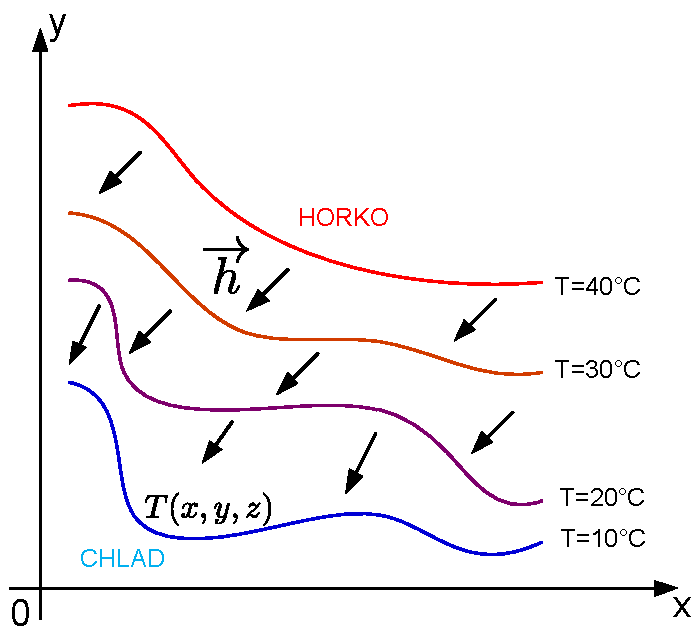
\includegraphics[width=0.5\linewidth]{fyz_fig0152.pdf}
        \caption{Teplota je příkladem skalárního pole. Každému bodu $(x,y,z)$ v prostoru je 
                přiřazeno číslo $T(x,y,z)$. Všechny body na ploše označené $T = 20°C$ (zobrazené 
                jako křivka při $z=0$) mají stejnou teplotu. Šipky jsou ukázkami hustoty tepelného 
                toku $\vec{h}$.
                \cite[s.~29]{Feynman02}}
        \label{fyz:fig0152} 
      \end{figure}
            
      U \textbf{vektorových polí} je v každém bodě prostoru dán vektor, který se mění od bodu k
      bodu. Jako příklad vezměme rotující těleso (obr. \ref{fyz:fig0032}). Rychlost látky, tvořící
      těleso je v každém bodě vektor, který je funkcí polohy. V druhém případě uvažujme proudění
      tepla z teplejších míst do chladnějších. V různých částech uvažovaného tělesa bude teplo
      proudit různými směry. \emph{Hustota tepelného toku} je veličina, která se vyznačuje směrem.
      Označme ji $\vec{h}$. Její velikost je mírou proudícího tepla. Vektor hustoty tepelného toku
      je vyznačen pro několik poloh i na obr. \ref{fyz:fig0152}. Definujeme $\vec{h}$ přesněji.
      Velikost vektoru hustoty tepelného toku udává tepelnou energii, která projde infinitezimálním
      plošným elementem postaveným kolmo na směr toku za jednotku času přepočtenou na  jednotku
      plochy. Vektor má směr toku (obr. \ref{fyz:fig0153a}). Vyjádříme to v symbolech: je-li $\Delta
      P$ tepelná energie, která projde za jednotku času
      \begin{equation*}     % \label{temp:eq_tepelny_tok}
        \vec{h}=\frac{\Delta P}{\Delta S}\vec{e_t}
                \quad \vec{e_t}\ldots\text{jednotkový vektor ve směru toku}
      \end{equation*}   
  
      \luagraphic[0.7]{fyz_fig0032.pdf}{Rychlost v rotujícím tělese je příkladem vektorového pole.
      \cite[s.~30]{Feynman02}}{fyz:fig0032}
            
      Vektor $\vec{h}$ je možno definovat i jiným způsobem - pomocí jeho složek. Ptejme se, kolik 
      tepla projde malou ploškou postavenou pod libovolným úhlem vzhledem k toku. Obrázek 
      \ref{fyz:fig0153b} znázorňuje plošku $\Delta S_2$ skloněnou pod úhlem $\Theta$ k plošce 
      $\Delta S_1$ kolmé na tok. Jednotkový vektor $\vec{n}$ je kolmý na plošku $\Delta S_2$. 
      Vektory $\vec{n}$ a $\vec{h}$ svírají úhel $\Theta$ (neboť $\vec{h}$ je kolmé $\Delta 
      S_1$). Jaká je nyní hustota tepelného toku ploškou $\Delta S_2$? Tok ploškou $\Delta S_2$ je 
      stejný jako ploškou $\Delta S_1$, pouze velikosti obou plošek jsou odlišné, a to $\Delta 
      S_1=\Delta S_2\cos\Theta$. Hustota toku ploškou $\Delta S_2$ je 
      \begin{equation}\label{fyz:eq248}
        \frac{\Delta P}{\Delta S_2}=\frac{\Delta P}{\Delta S_1}\cos{\Theta}=\vec{h}\cdot\vec{n}
      \end{equation}
  
      \begin{figure}[ht!]
        \centering
        \subcaptionbox{\label{fyz:fig0153a}}{\luafigure[0.7]{fyz_fig0153a_ver1.pdf}} \\                                          
        \subcaptionbox{\label{fyz:fig0153b}}{\luafigure[0.5]{fyz_fig0153b_ver1.pdf}}
        \caption{a) Vektor hustota tepelného toku $\vec{h}$ ukazuje směr proudění. Jeho velikost
                  je rovna energii, která za jednotku času projde elementární ploškou postavenou 
                  kolmo na směr proudění, vydělené obsahem této plošky. b) Tepelný tok ploškou 
                  $\Delta S_2$ je stejný jako tepelný tok ploškou $\Delta S_1$.
                  \cite[s.~30]{Feynman02}}
        \label{fyz:fig0153}
      \end{figure}
      
      Tuto rovnici interpretuje tak, že hustotu tepelného toku $\vec{h}$ (teplo prošlé za jednotku 
      času jednotkovou plochou) libovolnou elementární ploškou, jejíž jednotkový normálový vektor 
      je $\vec{n}$, udává výraz $\vec{h}\cdot\vec{n}$. Taktéž bychom mohli říci: složka hustoty 
      tepelného toku kolmá na elementární plošku $\Delta S_2$ je $\vec{h}\cdot\vec{n}$. Chceme-li, 
      můžeme považovat tyto výro\-ky za definice $\vec{h}$. Stejné představy můžeme použít i pro 
      jiná vektorová pole.
          
    % ------------------------ Derivace polí - gradient ----------------------------------------------
    \subsection{Derivace polí - gradient}\label{fyz:IIchapIIsecIV}
      Mění-li se pole s časem, je možné udávat tyto změny pomocí jejich derivace podle času. Podobným 
      způsobem chceme popsat jejich změny v závislosti na poloze, protože se, řekněme, zajímáme o 
      vztah teploty v jednom místě k teplotě v sousedním místě. Jak vypočteme derivaci teploty podle 
      polohy? Máme derivovat podle \(x\)? Nebo podle \(y\), nebo $z$?
    
      Užitečné fyzikální zákony nezávisí na orientaci souřadnicové soustavy. Proto se musí zapisovat 
      ve tvaru, v němž jsou obě strany buď skaláry, nebo vektory. Co je derivace skalárního pole, 
      například $\pder{T}{x}$. Je to skalár nebo něco jiného? Můžeme se snadno přesvědčit, že to není 
      ani skalár ani vektor, neboť vezmeme-li jinou osu \(x\), $\pder{T}{x}$ se jistě změní. Ale 
      všimněme si, že máme tři možné derivace: $\pder{T}{x},\,\pder{T}{y},\,\pder{T}{z}$. Protože 
      existují tři derivace a víme, že tři čísla tvoří vektor, tyto tři derivace by mohly 
      představovat složky jednoho vektoru:
      \begin{equation}\label{fyz:eq249}
        \left(\pder{T}{x},\,\pder{T}{y},\,\pder{T}{z}\right)\overset{?}{=}\mathrm{vektor}
      \end{equation}
      Samozřejmě, ne každá tři čísla obecně tvoří vektor. Je tomu tak pouze tehdy, když při pootočení
      souřadnicové soustavy se složky vektoru správně transformují. Proto je nevyhnutelné prozkoumat, 
      jak se naše tři derivace změní při otočení souřadnicové soustavy. Ukážeme, že rov.     
      \ref{fyz:eq249} je skutečně vektorem. Při otáčení souřadnicové soustavy se derivace    
      transformují správně.
    
      Můžeme se o tom přesvědčit několika způsoby. Jeden způsob je položit si takovou otázku, na níž 
      lze odpovědět nezávisle na souřadnicové soustavě, a pokusit se vy\-já\-dřit odpověď v 
      "invariantním" tvaru. Například jsou-li $\vec{A}$ a  $\vec{B}$ vektory a 
      $S=\vec{A}\cdot\vec{B}$, víme, že $S$ je skalárem. I bez zjišťování \emph{víme}, zda se $S$ 
      mění se změnou souřadnicových soustav. \emph{Nemůže}, neboť jde o skalární součin dvou vektorů. 
      Podobně, \emph{víme-li}, že \(\vec{A}\) je vektorem a mám tři čísla \(B_1\), \(B_2\) a \(B_3\), 
      o kterých zjistíme že
      \begin{equation}\label{fyz:eq250}
        A_xB_1+A_yB_2+A_zB_3=S
      \end{equation}
      kde \(S\) je totéž pro libovolnou souřadnicovou soustavu, pak tři čísla $B_1$, $B_2$ a $B_3$ 
      jsou nutně složkami $B_x$, $B_y$ a $B_z$  nějakého vektoru $\vec{B}$.
    
      Zvažme případ teplotního pole. Vez\-mě\-me dva body $P_1$ a $P_2$ v malé vzdálenosti 
      $\Delta\vec{r}$ od sebe. Teplota v $P_1$ je $T_1$ a v $P_2$ je $T_2$ s rozdílem $\Delta 
      T=T_2-T_1$. Teploty v těchto reálných, fyzikálních bodech určitě nezávisí na volbě os 
      souřadnic. Konkrétně $\Delta T$ je číslo nezávislé na souřadnicové soustavě. Je to skalár.
  
      \begin{figure}[ht!]  %\ref{fyz:fig0031}
        \centering
        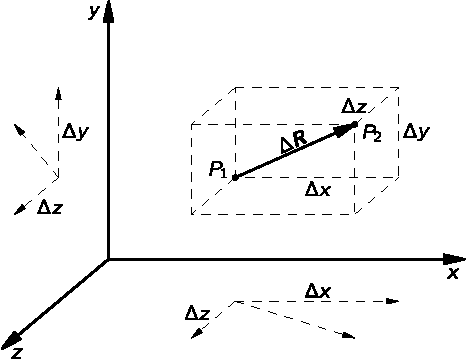
\includegraphics[width=0.6\linewidth]{fyz_fig0031_ver1.pdf}
        \caption{Vektor $\vec{r}$, jehož složky jsou $\Delta x,\,\Delta y,\,\Delta z$.}
        \label{fyz:fig0031}
      \end{figure}
      Zvolíme-li nějakou vhodnou soustavu souřadnicových os, můžeme napsat $T_1=T(x,y,z)$ a 
      $T_2=T(x+\Delta x,\,y+\Delta y,\,z+\Delta z)$, kde $\Delta x,\,\Delta y,\,\Delta z$ jsou složky 
      vektoru $\Delta \vec{r}$ (obr. \ref{fyz:fig0031}). Vzhledem k rovnosti rov. 
      \ref{fyz:eq245} můžeme psát    
      \begin{equation}\label{fyz:eq251}
        \Delta T = \pder{T}{x}\Delta x + \pder{T}{y}\Delta y + \pder{T}{z}\Delta z
      \end{equation}
      Levá strana rovnosti (\ref{fyz:eq251}) je skalárem. Pravá je součtem tří součinů obsahujících 
      jako součinitele $\Delta x,\,\Delta y,\,\Delta z$, které jsou složkami vektoru. Z toho vyplývá, 
      že tři čísla \(\frac{\partial T}{\partial x},\,\frac{\partial T}{\partial y},\,\frac{\partial 
      T}{\partial z}\) Představují také \(x\)-ovou, \(y\)-ovou a \(z\)-ovou složku nějakého vektoru. 
      Pro tento nový vektor použijeme symbol \(\nabla T\). Symbol \(\nabla\) (nazývaný \uv{nabla}) je 
      převráceným \(\Delta\) a má připomínat derivování. \(\nabla T\) se čte různě: \emph{\uv{nabla 
      T}} nebo \emph{\uv{gradient T}} nebo \emph{\uv{grad T}};
      \begin{equation}\label{fyz:eq252}
        \mathrm{grad}\,T =\nabla T = \left(\pder{T}{x},\, \pder{T}{y},\,\pder{T}{z} \right)
        \protect\footnotemark[4]
      \end{equation}
      \footnotetext[4]{V naší symbolice představuje výraz \((a, b, c)\) vektor se složkami \(a\),
      \(b\), \(c\). Použijeme-li jednotkové vektory $\vec{i},\,\vec{j},\,\vec{k}$, můžeme psát
      $$\mathrm{grad}\,T=\nabla T = \vec{i}\pder{T}{x} + \vec{j}\pder{T}{y} + \vec{k}\pder{T}{z}$$}
      Použitím této nové symboliky se můžeme pokusit rovnost (\ref{fyz:eq251}) 
      přepsat na kompaktnější tvar
      \begin{equation}\label{fyz:eq257}
        \Delta T = \nabla T \cdot\Delta\vec{r}
      \end{equation}        
  
      \begin{figure}[ht!]
        \centering
        \subcaptionbox{\label{fyz:fig0154a}}{\luafigure[0.45]{fyz_fig0154a_ver1.pdf}}
        \subcaptionbox{\label{fyz:fig0154b}}{\luafigure[0.45]{fyz_fig0154b_ver1.pdf}}
        \caption{Užitečné fyzikální zákony nezávisí na orientaci souřadnicové soustavy. Dokažme to!
                  a) Transformace do pootočené souřadnicové soustavy; b) Speciální případ, v němž je 
                  vektor \(\vec{r}\) rovnoběžný s osou \(x\).
                  \cite[s.~33]{Feynman02}}
        \label{fyz:fig0154}
      \end{figure}
  
      Tento vztah, vyjádřený slovy, říká, že rozdíl teplot ve dvou sousedních bodech je roven 
      skalárnímu součinu gradientu $T$ a rozdílu polohových vektorů obou bodů. Tvar rov. 
      \ref{fyz:eq257} také ilustruje již uvedený důkaz, že  $\nabla T$ je opravdu vektorem.
  
      Stále ještě nejste přesvědčeni? Ukážeme, že složky $\nabla T$ se transformují stejně jako 
      složky $\vec{r}$. Pokud ano, $\nabla T$ je vektor podle naší původní definice vektoru. Abychom 
      si to trochu zjednodušili, položme $z=z'$, takže souřadnici $z$ již nemusíme brát v úvahu.
  
      Uvažujme o soustavě $x'$, $y'$ pootočené o úhel $\Theta$  vzhledem k soustavě $xy$ (obr.
      \ref{fyz:fig0154}). Souřadnice bodu $(x,y)$ vyjádřené v čárkované soustavě jsou
      \begin{alignat*}{3}
        x' &=  &&x\cos\Theta &&+ y\sin\Theta             \\
        y' &= -&&x\sin\Theta &&+ y\cos\Theta,            
      \end{alignat*}
      vyjádříme-li \(x\) a \(y\)
      \begin{alignat}{3}
        x  &= &&x'\cos\Theta &&- y'\sin\Theta    \label{fyz:eq253}\\
        y  &= &&x'\sin\Theta &&+ y'\cos\Theta.  \nonumber
      \end{alignat}
      Transformují-li se nějaká dvojice čísel podle těchto rovnic stejně jako \(x\) a \(y\), jde o složky
      vektoru.
  
      Nyní si všimněme rozdílu teplot ve dvou sousedních bodech $P_1$ a $P_2$, zvolených tak, jak to
      znázorňuje obr. \ref{fyz:fig0154b}. Při výpočtu v souřadnicích \(x\) a \(y\) můžeme psát
      \begin{align}
        \Delta T  &= \pder{T}{x}\Delta x \quad
                      \text{neboť} \quad \Delta y=0.   \label{fyz:eq254} \\ 
        \shortintertext{A výpočet v čárkované soustavě? Tam bychom psali}
        \Delta T  &= \pder{T}{x'}\Delta x' +
                      \pder{T}{y'}\Delta y'      \label{fyz:eq255}   \\
        \shortintertext{Podíváme-li se na obr. \ref{fyz:fig0154b}, vidíme, že}
        \Delta x' &=  \Delta x\cos\Theta \quad \Delta y' = -\Delta x\sin\Theta
      \end{align}
      neboť $\Delta y'$ je záporné při kladném $\Delta x$. Dosazením těchto výrazů do rov.    
      \ref{fyz:eq255} dostaneme
      \begin{align}
        \Delta T    &=  \pder{T}{x'}\Delta x\cos\Theta
                        -\pder{T}{y'}\Delta x\sin\Theta   \nonumber \\
                    &=  \left(\pder{T}{x'}\cos\Theta   -
                        \pder{T}{x'}\sin\Theta\right)\Delta x  \label{fyz:eq256} \\
        \shortintertext{Porovnáním rov. \ref{fyz:eq256} s rov.   
                        \ref{fyz:eq254} zjistíme, že}
        \pder{T}{x} &=  \pder{T}{x'}\cos\Theta - \pder{T}{y'}\sin\Theta. \label{temp:eq_pT_px}
      \end{align}
      Podle tohoto vztahu $\pder{T}{x}$ dostaneme z $\pder{T}{x'}$ a $\pder{T}{y'}$ právě tak jako 
      \(x\) z $x'$ a $y'$ (rov. \ref{fyz:eq253}). $\pder{T}{x}$ je tedy $x-\text{ovou}$ složkou 
      vektoru. Podobné úvahy by ukázaly, že $\frac{\partial T}{\partial y}$ je $y-\text{ová}$ a 
      $\pder{T}{z}$ jeho $z-\text{ová}$ složka. $\nabla T$ je zajisté vektorem. Jde o vektorové pole 
      odvozené ze skalárního pole $T$.
          
    % ------------------------ Operátor nabla ------------------------------------------------------- 
    \subsection{Operátor \texorpdfstring{\fontsize{11pt}{12pt}\selectfont\(\nabla\)}{nabla}}\label{fyz:IIchapIIsecV}
      Důkaz, že $\grad{T}$ nebo $\nabla T$ je vektorem, nezávisí na tom, jaké skalární pole jsme 
      derivovali. Všechny úvahy by byly stejné i tehdy, kdyby se $T$ zaměnilo za jakékoliv jiné 
      skalární pole. Transformační rovnice jsou stejné bez ohledu na to, co derivujeme, mohli bychom 
      $T$ vynechat a nahradit rovnici (\ref{temp:eq_pT_px}) operátorovou rovnicí
      \begin{equation}\label{temp:eq_operatorova_rce}
        \pder{ }{x}=\pder{ }{x'}\cos\Theta - \pder{ }{y'}\sin\Theta.
      \end{equation}
      Ponecháme přitom operátory "hladové po derivování".
  
      Protože diferenciální operátory samotné se transformují stejně jako složky vektoru, můžeme jej 
      nazvat složkami \emph{vektorového operátoru}. Můžeme psát
      \begin{align}
        \nabla   &= \left(\pder{ }{x},\,\pder{ }{y},\,\pder{ }{z}\right)       \label{fyz:eq258}\\
        \shortintertext{což samozřejmě znamená, že}
        \nabla_x &= \pder{ }{x},\quad \nabla_y=\pder{ }{y},\quad\nabla_z=\pder{ }{z}.
      \end{align}  
      Gradient jsme abstrahovali od \(T\).
  
      Musíme si uvědomit, že operátorová algebra je trochu odlišná od vektorové algebry. S operátory 
      vždy musíme dodržovat správné pořadí, aby operace s nimi měly ten pravý smysl. Co se má 
      derivovat, musí se umístit napravo od $\nabla$. $T\nabla$ je stále operátorem, zatímco $\nabla 
      T$ už není "hladovým" operátorem, neboť se nasytil. Je to opravdový fyzikální vektor, 
      představující rychlost změny $T$ v prostoru. Víme, že rychlost změny $T$ v nějakém směru udává 
      složka vektoru $\nabla T$ v tomto směru (viz vztah \ref{fyz:eq257}). Z toho vyplývá, že 
      $\nabla T$ směřuje tam, kde má největší možnou složku - jinými slovy, směrem, v němž se $T$ 
      mění nejrychleji. \textbf{Gradient $T$ má směr nej\-rychlejšího zvětšo\-vání veličiny $T$.}
      
      % ---------------------- Operace s nabla -------------------------------------------------------
      \subsubsection{Operace s \texorpdfstring{\(\nabla\)}{nabla}}
        Je možné s vektorovým operátorem $\nabla$ provádět nějaké jiné algebraické operace? Pokusme 
        se kombinovat jej s nějakým vektorem. Dva vektory se kombinují vy\-já\-dře\-ním skalárního 
        součinu. Mohly bychom vytvořit dva součiny
        \begin{equation}\label{fyz:eq259}
          (\mathrm{vektor})\cdot\nabla\quad\mathrm{nebo}\quad\nabla\cdot(\mathrm{vektor})
        \end{equation}
        První součin zatím neznamená nic, protože je to stále pouhý operátor. Jeho konečný smysl by 
        závisel na tom, na co se má aplikovat. Druhý součin je jakési skalární pole. 
        ($(\vec{A}\cdot\vec{B})$ je vždy skalárem.)
  
        Prozkoumejme skalární součin operátoru $\nabla$ s vektorovým polem, které známe, např. 
        $\vec{h}$.  Vypíšeme-li ho ve složkách
        \begin{align}
          \ndiver{h} &= \nabla_x\cdot h_x +
                        \nabla_y\cdot h_y +
                        \nabla_z\cdot h_z               \label{fyz:eq260}     \\
          \shortintertext{nebo}
          \ndiver{h} &= \pder{h_x}{x} +
                        \pder{h_y}{y} +
                        \pder{h_z}{z}                   \label{fyz:eq261}
        \end{align}
        Tento součet je invariantní vzhledem k transformaci souřadnic. Kdybychom zvolili jinou
        souřadnicovou soustavu (označenou čárkami), dostali bychom\footnote{Na $\vec{h}$ se díváme
        jako na fyzikální veličinu, která závisí na poloze v prostoru, a ne, přesně vzato, jako na
        matematickou funkci tří proměnných. Když je $\vec{h}$ "derivováno" podle \(x\),\(y\) a $z$
        nebo podle $x'$ ,$y'$ a $z'$, je třeba nejdříve vyjádřit matematický výraz pro $\vec{h}$
        jako funkci příslušných proměnných. Proto v této nové souřadnicové soustavě neoznačujeme
        $\vec{h}$ čárkou.}
        \begin{equation}\label{fyz:eq262}
          \nabla'\cdot\vec{h}=\pder{h_{x'}}{x'}+\pder{h_{y'}}{y'}+\pder{h_{z'}}{z'}
        \end{equation}
        což je totéž číslo, které bychom dostali z (rov. \ref{fyz:eq261}), přestože 
        tento vztah vypadá jinak. To znamená, že
        \begin{equation}\label{fyz:eq263}
            \nabla'\cdot\vec{h}= \ndiver{h}
        \end{equation}
        pro každý bod prostoru. Tedy $\nabla\cdot\vec{h}$ je skalární pole, které musí reprezentovat
        nějakou fyzikální veličinu. Musíte si uvědomit, že kombinace derivací $\nabla\cdot\vec{h}$
        je dost specifická.  Existují rozmanité kombinace, např. $\pder{h_y}{x}$, které nejsou ani
        skaláry, ani složkami vektorů.
  
        Skalární veličina $\nabla\cdot(\text{vektor})$ je ve fyzice neobyčejně užitečná. Byla
        nazvána \textbf{divergencí} ($\diver{h}$). Například
        \begin{equation}\label{fyz:eq264}
          \ndiver{h}= \diver{h}=\text{divergence}\, \vec{h}.
        \end{equation}
        Podobně jako v případě $\nabla T$ můžeme najít fyzikální význam i pro $\nabla\cdot\vec{h}$.
        Odložíme to však na později.
  
        Nejdříve se chceme podívat, co můžeme ještě vymyslet pomocí vektorového operátoru $\nabla$. 
        Jak je to s jeho vektorovým součinem? Je třeba očekávat, že
        \begin{equation}\label{fyz:eq265}
          \nrot{h} = \text{vektor}
        \end{equation}
        Složky tohoto vektoru můžeme rozepsat podle obyčejného pravidla pro vektorové součiny (viz 
        rov. \ref{fyz:eq690}).
        \begin{align*}
          (\nrot{h})_x &= \nabla_yh_z-\nabla_zh_y = \pder{h_z}{y} - \pder{h_y}{z} \\
          (\nrot{h})_y &= \nabla_zh_x-\nabla_xh_z = \pder{h_x}{z} - \pder{h_z}{x} \\
          (\nrot{h})_z &= \nabla_xh_y-\nabla_yh_x = \pder{h_y}{x} - \pder{h_x}{y}
        \end{align*}
  
        Kombinace $\nabla\times\vec{h}$ se nazývá \textbf{rotace} $\vec{h}$
        ($\mathrm{rot}\,\vec{h}$). O příčině tohoto pojmenování a o fyzikálním významu této
        kombinace pojednáme později.
  
        Celkově tedy máme tři různé kombinace, v nichž vystupuje operátor $\nabla$:
        \begin{align*}
          \ngrad{T}  &=\grad{T}   = \text{vektor} \\    
          \ndiver{h} &=\diver{h}  = \text{skalár} \\  
          \nrot{h}   &=\rot{h}    = \text{vektor}
        \end{align*}
        Pomocí těchto kombinací můžeme popsat prostorové změny polí ve vhodném tvaru, tj. obecném 
        tvaru, nezávislém na nějaké souřadnicové soustavě.
  
        Jako příklad použití našeho vektorového diferenciálního operátoru $\nabla$ napíšeme soustavu
        vektorových rovnic obsahujících tytéž zákony elektromagnetizmu - Maxwellovy rovnice:
        \begin{equation}\label{fyz:eq266}
          \begin{array}{c @{{}={}} l r @{{}={}} l}
            \ndiver{E} & \dfrac{\rho}{\varepsilon_0}& \ndiver{B}   & 0,                          \\
            \nrot{E}   & -\pder{\vec{B}}{t}   \quad\quad\quad   & c^2\nabla\times\vec{B} & 
            \pder{\vec{E}}{t} + \frac{\vec{j}}{\varepsilon_0}  
          \end{array}
        \end{equation}
  
        kde $\rho$ (ró) je hustota elektrického náboje, tj. množství náboje v jednotce objemu,
        $\vec{j}$ je hustota elektrického proudu, tj. množství náboje, které proteče jednotkovou
        plochou za sekundu. Tyto čtyři rovnice obsahují úplnou klasickou teorii elektromagnetického
        pole. Vidíte, jakého elegantního a jednoduchého zápisu můžeme dosáhnout pomocí naší nové
        symboliky.
        
    % -------- Diferenciální rovnice proudění tepla --------------------------------------------------
    \subsection{Diferenciální rovnice proudění tepla}\label{fyz:IIchapIIsecVI}
      Uveďme jiný příklad fyzikálního zákona napsaného ve vektorové symbolice. Není to obecně platný 
      zákon, ale pro mnohé kovy a mnoho dalších látek, jež jsou vodiči tepla, je dost přesný. 
      Vezmeme-li kus materiálu v podobě desky a jeho čelní stěnu zahřejeme na teplotu $T_2$, zatímco 
      protilehlou stranu ochladíme na odlišnou teplotu $T_1$, materiálem bude proudit teplo ve směru 
      od $T_2$ k $T_1$ (obr. \ref{fyz:fig0155}).
      
      Tepelný tok je přímo úměrný plošnému obsahu $S$ stěn i rozdílu teplot $T_2-T_1$ a nepřímo 
      úměrný vzdálenosti $d$ mezi stěnami. (Pro daný rozdíl teplot platí, že čím tenčí je deska, tím 
      větší je tepelný tok). Nechť $P$ je tepelná energie, která projde deskou za jednotku času. 
      Potom můžeme napsat
      \begin{equation}\label{fyz:eq684}
        \Delta P=\lambda(T_2-T_1)\frac{S}{d},
      \end{equation}
      Konstanta úměrnosti $\lambda$ (lambda) se nazývá \emph{součinitel teplotní vodivosti}.
      
      Co se stane ve složitějším případě, řekněme v tělese nepravidelném tvaru, v jehož objemu se 
      teplota různě mění? Uvažujme kousíček tělesa a představme si v něm takovou destičku, jaká je 
      nakreslená na obr. \ref{fyz:fig0155a}, ale v miniaturním měřítku. Nasměrujeme její čelní 
      stěny rovnoběžně s izotermickými hladinami obr. \ref{fyz:fig0155b}, takže pro destičku bude 
      platit rov. \ref{fyz:eq684}.
      
      Je-li plošný obsah čelní stěny destičky $\Delta S$, je tepelný tok
      \begin{equation}\label{fyz:eq683}
        P=\lambda(\Delta T)\frac{\Delta S}{\Delta d}
      \end{equation}
      kde $\Delta d$ je tloušťka destičky. $\dfrac{\Delta P}{\Delta S}$ jsme definovali jako velikost
      vektoru $\vec{h}$ ležícího ve směru tepelného toku. 
  
      \begin{figure}[ht!]
        \centering
        \subcaptionbox{\label{fyz:fig0155a}}{\luafigure[0.4]{fyz_fig0155a.pdf}}
        \subcaptionbox{\label{fyz:fig0155b}}{\luafigure[0.4]{fyz_fig0155b.pdf}}
        \caption{a) Tepelný tok deskou. b) Infinitezimální destička rovnoběžná s izotermickou 
                  hladinou ve velkém kuse látky \cite[s.~38]{Feynman02}}
        \label{fyz:fig0155}
      \end{figure}
  
      Teplo bude proudit od $T_1+\Delta T_1$ k $T_1$ a tudíž kolmo na izotermy (obr.
      \ref{fyz:fig0155b}). $\dfrac{\Delta P}{\Delta d}$ udává dále právě rychlost změny $T$ při změně
      polohy. Protože poloha se mění ve směru kolmém na izotermy, naše $\dfrac{\Delta T}{\Delta d}$
      udává maximální rychlost změny $T$, a tedy velikost vektoru $\nabla T$. Protože směr $\nabla T$
      je opačný než směr\footnote{Záporné znaménko je nutné, neboť teplo proudí ve směru poklesu
      teploty.} $\vec{h}$  rov. \ref{fyz:eq683} zapsaná pomocí vektorů bude vypadá takto
      \begin{equation}\label{fyz:eq685}
        \vec{h}=-\lambda\nabla T
      \end{equation}
      Rovnice \ref{fyz:eq685} je diferenciální rovnicí vedení tepla v masivních 
      tělesech. Jde o skutečnou vektorovou rovnici. Každá její strana je vektor, je-li $\lambda$ jen 
      číslo. Je zobecněním speciální rov. \ref{fyz:eq683} pro pravoúhlé desky na 
      libovolné případy. Tato symbolika je užitečný nejen proto, že v ní rovnice vypadají 
      jednodušeji, ale i proto, že nejjasněji ukazuje fyzikální obsah rovnic bez odvolání na nějakou 
      libovolně zvolenou souřadnicovou soustavu.      
      
    %---------------- Druhé derivace vektorových polí ------------------------------------------------
    \subsection{Druhé derivace vektorových polí}\label{fyz:IIchapIIsecVII}
      Dosud jsme měli pouze první derivace. Proč se však nezabývat i druhými derivacemi? Mohli bychom
      sestavit několik kombinací:
      \begin{enumerate}[leftmargin=2cm,rightmargin=2cm, label=\emph{\alph*}),noitemsep]
        \setlength{\itemsep}{0cm}%
        \setlength{\parskip}{0em}%
        \item $\nabla\cdot(\nabla T)$
        \item $\nabla\times(\nabla T)$
        \item $\nabla\cdot(\ndiver{h})$
        \item $\nabla\cdot(\nrot{h})$
        \item $\nabla\times(\nrot{h})$
      \end{enumerate}
      Můžeme se přesvědčit, že to jsou všechny možné kombinace.
    
      Podívejme se nejdříve na druhou z nich, tj. na b). Má stejný tvar jako 
      $\vec{A}\times(\vec{A}T)= (\vec{A}\times\vec{A})T = 0$, neboť $\vec{A}\times\vec{A}$ je 
      vždy \(0\). Z toho tedy vyplývá, že
      \begin{equation}\label{fyz:eq239}
        \mathrm{rot}\,\grad{T} = \nabla\times\nabla T = 0.
      \end{equation}
      Jak dochází k této rovnosti, můžeme vidět, když si výraz b) napíšeme ve složkách: 
      \begin{align*}
        [\nabla\times(\nabla T)]_z 
            &= \nabla_x(\nabla T)_y-\nabla_y(\nabla T)_x                                   \\
            &= \pder{}{x}\left(\pder{T}{y}\right) - \pder{}{y}\left(\pder{T}{x}\right)
      \end{align*}
      což je nula podle rovnosti (\ref{fyz:eq246}). Stejně je to pro další složky.
      \(\nabla\times(\nabla T)=0\) tedy platí pro jakékoliv rozdělení teploty - dokonce pro 
      \emph{jakoukoliv} skalární funkci.
    
      Vezměme si jiný příklad. Podívejme se, zda se nám podaří dostat i jiný výraz rovný nule. 
      Skalární součin vektoru s vektorovým součinem obsahující tentýž vektor dává nulu
      \begin{equation*}
        \vec{A}\cdot(\vec{A}\times\vec{B}) = 0
      \end{equation*}
      neboť \((\vec{A}\times\vec{B})\) je kolmé na \(\vec{A}\) a jeho složka ve směru \(\vec{A}\) je 
      tedy nulová. Stejná kombinace se vyskytuje v rovnici d), a tak dostáváme
      \begin{equation}\label{fyz:eq686}
        \nabla\cdot(\nabla\times\vec{h}) = \mathrm{div}\,(\rot{h})= 0.
      \end{equation}
      Snadno se opět ukáže, že je to \(0\), zapíší-li se naznačené operace ve složkách.
    
      Nyní zformulujeme dvě matematické věty, které nebudeme dokazovat. Jsou to velice zajímavé věty 
      a je pro fyziky užitečné je znát. 
    
      Ve fyzikálních úlohách často zjistíme, že rotace nějaké veličiny, řekněme vektorového pole 
      \(\vec{A}\), je nula. Viděli jsme (rovnost \ref{fyz:eq239}), že rotace gradientu je rovna 
      nule, což se vzhledem k vlastnostem vektorů dobře pamatuje. Bylo by tedy dobře možné, aby bylo 
      \(\vec{A}\) gradientem nějaké veličiny; jeho rotace by pak byla nutně nulová. Platí zajímavá 
      věta, podle které, je-li \(\rot{A}\) rovna nule, je \(\vec{A}\) vždy gradientem něčeho, a tedy 
      existuje určité skalární pole \(\Psi\) (psí) takové, že \(\vec{A}\) je rovno \(\grad{\Psi}\) 
      Jinými slovy platí následující věta
      \begin{lemma}
        Je-li $\nabla\times\vec{A}=0$, existuje $\psi$ takové, že $\vec{A} = \nabla\psi$
      \end{lemma}
      Podobná věta platí i v případě, že div A je rovna nule. Rovnost (\ref{fyz:eq686}) říká, že
      divergence rotace něčeho je vždy nula. Setkáme-li se s vektorovým polem \(\vec{D}\), přičemž 
      \(\diver{D}\) je rovna nule, můžeme z toho usoudit, že \(\vec{D}\) je rotací nějakého vektorového pole 
      \(\vec{C}\).
      \begin{lemma}
        Je-li $\diver{D} = 0$, existuje $\vec{C}$ takové, že $\vec{D} = \nabla\times\vec{C}$.
      \end{lemma}
      Při zkoumání možných kombinací dvou operátorů \(\nabla\) jsme zjistili, že dvě z nich dávají 
      vždy nulu. Podívejme se nyní na ty, které nejsou nulové. Vezměme kombinaci 
      \(\nabla\cdot(\ngrad{T})\), která byla v našem záznamu napsaná jako první. Obecně nulu nedává. 
      Vypíšeme složky: 
      \begin{align*}
        \ngrad{T}              &= (\nabla_xT, \nabla_yT, \nabla_zT).  \\
        \shortintertext{Potom}
        \nabla\times(\nabla T) &= \nabla_x(\nabla_xT) + \nabla_y(\nabla_yT) + \nabla_z(\nabla_zT)   \\
                                &= \ppder{T}{x} + \ppder{T}{y} + \ppder{T}{z}.
      \end{align*}
      z čehož v obecném případě dostaneme nějaké číslo. Jde o skalární pole. 
    
      Vidíme, že není třeba ani dávat závorky a aniž bychom riskovali záměnu, můžeme psát \(\nabla 
      \cdot(\nabla T) = (\nabla\cdot\nabla)T = \nabla\cdot\nabla T = \nabla^2T\). Na \(\nabla^2\) se 
      díváme jako na nový operátor - \textbf{Laplaceův operátor}:
      \begin{equation}\label{fyz:eq687}
        \nabla^2 = \ppder{}{x} + \ppder{}{y} + \ppder{}{z}.
      \end{equation}
      Protože Laplaceův operátor je skalárním operátorem, můžeme jím působit i na vektor - myslíme 
      tím tutéž operaci na každou složku vektoru v pravoúhlé souřadnicové soustavě:
      \begin{equation*}
        \nabla^2\vec{h} = (\nabla^2h_x, \nabla^2h_y, \nabla^2h_z).
      \end{equation*}
      Podívejme se na další možnost, kterou je rovnice e), tj. \(\nabla\times\nabla\times\vec{h}\). 
      Vzhledem k vektorové rovností (\ref{fey:eq_baccab}) můžeme rotaci vyjádřit jinak. Při použití 
      výše této rovnice 
      musíme \(\vec{A}\) a \(\vec{B}\) nahradit operátorem \(\nabla\) a položit \(\vec{C} = \vec{h}\).
      \begin{equation*}
        \nabla\times(\nrot{h}) = \nabla(\nabla\cdot\vec{C}) - \vec{h}(\nabla\cdot\nabla) \ldots ???
      \end{equation*}
      Okamžik! Něco je špatně. První dva členy jsou totiž vektory, jak to má být (operátory v nich 
      jsou „nasycené“), ale poslední člen není v pořádku. Má stále charakter operátoru. Chyba je v 
      tom, že jsme nebyli dost pozorní při dodržování pořadí symbolů v zápisech našich členů. Když si 
      znovu všimneme rovnosti (\ref{fey:eq_baccab}), zjistíme, že bychom ji mohli stejně dobře napsat 
      ve tvaru:
      \begin{align*}
        \vec{A}\times(\vec{B}\times\vec{C}) 
          &= \vec{B}\cdot(\vec{C}\cdot\vec{A}) - (\vec{A}\cdot\vec{B})\cdot\vec{C}  \\
        \shortintertext{Pořadí členů teď vypadá líp. Proveďme substituci do této rovnice. Dostáváme} 
        \nabla\times(\nabla\times\vec{h})
          &= \nabla(\ndiver{h}) - (\nabla\cdot\nabla)\vec{h} 
      \end{align*}
      Tento tvar se zdá být v pořádku. Skutečně je správný, o tom se můžete přesvědčit výpočtem 
      složek. Poslední člen je Laplaceův operátor a tak můžeme stejně dobře napsat
      \begin{equation*}
        \nabla\times(\nabla\times\vec{h}) = \nabla(\ndiver{h}) - \nabla^2\vec{h}.
      \end{equation*}
      Již jsme se zmínili o všech kombinacích v našem seznamu výrazů v úvodu kapitoly  
      \ref{fyz:IIchapIIsecVII} s dvojitým operátorem \(\nabla\) s výjimkou případu c), 
      tj.\(\nabla(\nabla\cdot\vec{h})\). To je přípustné vektorové pole, ale nic zvláštního se o něm 
      říci nedá. Jde pouze o určité vektorové pole, které se může příležitostně vyskytnout.
  
      Bude vhodné, když naše závěry shrneme:
      \begin{tcnote}
          \begin{alignat*}{2}
            \nabla\cdot(\nabla T)         &= \nabla^2 T && \ldots\text{skalární pole}    \\
            \nabla\times(\nabla T)        &= 0          &&                               \\
            \nabla\cdot(\ndiver{h})       &= ?          && \ldots\text{vektorové pole}   \\
            \nabla\cdot(\nrot{h})         &= 0          &&                               \\
            \nabla\times(\nrot{h})        &= \nabla(\ndiver{h}) - \nabla^2\vec{h}&&      \\
          (\nabla\cdot\nabla)\cdot\vec{h} &= \nabla^2\vec{h} && \ldots\text{vektorové pole}
          \end{alignat*}
      \end{tcnote}
      Všimněme si, že jsme se nepokusili zavést nový operátor \(\nabla\times\nabla\). Víme proč?
      
    %---------------- Nástrahy -----------------------------------------------------------------------
    \subsection{Nástrahy}\label{fyz:IIchapIIsecVIII}
      \cite[s.~41]{Feynman02} Naši znalost obvyklé vektorové algebry jsme aplikovali na algebru 
      operátoru \(\nabla\). Musíme přitom však být opatrní, neboť se můžeme dostat na scestí. Zmíníme 
      se o dvou nástrahách. V tomto kursu se však nevyskytnou. Co byste řekli následujícímu výrazu, 
      který obsahuje dvě skalární funkce \(\psi\) a \(\varphi\) (fí):
      \begin{align*}
        (\nabla\psi) &\times(\nabla\varphi)? 
        \shortintertext{Asi bychom chtěli prohlásit: musí to být nula, protože je to stejné jako}
        (\vec{A}a)   &\times(\vec{B}b),     
      \end{align*}
      což je rovno nule, neboť vektorový součin dvou stejných vektorů \(\vec{A}\times\vec{A}\) je 
      vždy nula. Ale v našem případě dva operátory \(\nabla\) nejsou stejné. První působí na jednu 
      funkci, a to \(\psi\), zatímco druhý působí na jinou funkci, tj. \(\varphi\). Proto ačkoliv je 
      označujeme tímtéž symbolem  \(\nabla\), je třeba o nich uvažovat jako o odlišných operátorech. 
      Je to pochopitelné, vždyť směr \(\nabla\psi\) závisí na funkci \(\psi\), a proto asi nebude 
      rovnoběžný s \(\nabla\varphi\).
      \begin{equation*}
        (\nabla\psi)\times(\nabla\varphi)\neq0 \text{ (obecně)}. 
      \end{equation*}
      My, naštěstí, nebudeme muset takové výrazy použít. (Co jsme právě řekli, nemění nic na faktu, 
      že \(\nabla\times\nabla(\psi)=0\) pro jakékoli skalární pole, neboť zde působí oba operátory 
      \(\nabla\) na stejnou funkci.)
  
      Nástraha číslo dvě (které se opět v kurzu vyhneme) spočívá v tomto: Pravidla, která jsme tu 
      uvedli, jsou jednoduchá a pěkná, když se použijí pravoúhlé souřadnice. Máme-li například 
      \(\nabla^2\vec{h}\) a potřebujeme složku \(x\), hned píšeme
      \begin{equation*}
        (\nabla^2\vec{h})_x = \left(\frac{\partial^2}{\partial x^2} + 
                                    \frac{\partial^2}{\partial y^2} + 
                                    \frac{\partial^2}{\partial z^2} 
                              \right)
      \end{equation*}
      Stejný výraz se však nedá napsat, kdybychom se ptali na radiální složku \(\nabla^2\vec{h}\). 
      Radiální složka \(\nabla^2\vec{h}\) není rovna výrazu \((\nabla^2\vec{h})_r\). Příčina je v 
      tom, že máme-li co dělat s vektorovou algebrou, jsou směry všech vektorů plně určeny. Ale pokud 
      jde o vektorová pole, jsou jejich směry v různých místech různé. Pokusíme-li se popsat 
      vektorové pole, řekněme v polárních souřadnicích, to, co nazýváme radiálním směrem, se od bodu 
      k bodu mění. Proto se můžeme dostat do velkých těžkostí, když začneme derivovat složky. 
      Například i pro konstantní vektorové pole se radiální složka bod od bodu mění.
  
      Obvykle je nejbezpečnější a nejjednodušší držet se pravoúhlých souřadnic a vyhnout se těžkostem.
      Je tu však jedna výjimka, která stojí za zmínku: Protože Laplaceův operátor \(\nabla^2\) je
      skalár, můžeme jej psát v souřadnicové soustavě jaké jen chceme (např. v polárních
      souřadnicích). Ale protože je to diferenciální operátor, smíme jej použít pouze na vektory,
      jejichž složky mají pevný směr, tj. na složky dané v pravoúhlé souřadnicové soustavě. Proto
      budeme-li naše vektorové diferenciální rovnice sát ve složkách, budeme všechna vektorová pole
      vyjadřovat pomocí jejich x-ových, y-ových a z-ových složek.
  
    \subsection{Cvičení}\label{fyz:IIchapIIsecIX}
      %---------------------------------------------------------------
      % !TeX spellcheck = cs_CZ
\begin{mdframed}[style=mdexam]
\begin{example}
  Jestliže platí, že \(\rot{A} = \rot{B}\), plyne z toho že \(\vec{A}=\vec{B}\)?\newline  
  \textbf{Řešení:} 
  Nikoliv. Mějme následující funkci \(\vec{A} = \vec{B} + \grad{\varPsi}\), kde 
  \(\varPsi(\vec{r})\) je libovolná skalární funkce (tedy \(\vec{A}\neq\vec{B}\)), pak platí
  \[\rot{A} = \rot{B} +\mathrm{rot}\;\grad{\varPsi} = \rot{B}\] (rotace gradientu je pro 
  spojité funkce vždy nulová, viz \ref{fyz:eq239} kapitola \ref{fyz:IIchapIIsecVII})
\end{example}
\end{mdframed}
      %---------------------------------------------------------------
      \begin{fyzexam}{Divergence el. pole bodového náboje}{exam009}
  Nalezněte divergenci elektrického pole bodového náboje v celém prostoru (pro 
  \textbf{bodový náboj} je \(r\rightarrow0\), \(\varrho\rightarrow\infty\)).
  (zdroj: \librariaALDBR)

\tcbsubtitle[before skip=\baselineskip]{Řešení:}  
  Elektrické pole v okolí bodového náboje je dáno \hyperlink{fyz:IIchapIVsecII}{Coulombovým zákonem}
  \[\vec{E} = \frac{Q}{4\cdot\pi\cdot r^2}\vec{n}_0,\] kde \(r\) je vzdálenost daného místa od
  náboje, \(\vec{n}_0\) je jednotkový vektor \(\vec{n}_0 = \left(\dfrac{x}{r}, \dfrac{y}{r},
  \dfrac{z}{r}\right)\) mířící od náboje. Elektrické pole má tedy složky \(\left(k =
  \dfrac{Q}{4\cdot\pi\cdot r^2}\right)\)
  \begin{equation*}
    E_x = k\left(\frac{x}{r^3}\right), \quad
    E_y = k\left(\frac{y}{r^3}\right), \quad
    E_z = k\left(\frac{z}{r^3}\right).
  \end{equation*}
  Pro výpočet divergence budeme potřebovat derivaci vzdálenosti podle jednotlivých
  proměnných:
  \begin{align*}
    \pder{r}{x} &= \pder{(x^2 + y^2 + z^2)^\frac{1}{2}}{x} = \frac{x}{r},  \\
    \pder{r}{y} &= \pder{(x^2 + y^2 + z^2)^\frac{1}{2}}{y} = \frac{y}{r},  \\ 
    \pder{r}{z} &= \pder{(x^2 + y^2 + z^2)^\frac{1}{2}}{z} = \frac{z}{r}.  \\
    \shortintertext{Divergence elektrického pole je, jak známo}            
    \diver{E}   &= \pder{E_x}{x} + \pder{E_y}{y} + \pder{E_z}{z}.
  \end{align*}
  Derivace jednotlivých složek je v tomto případě optimální řešit jako derivace podílu:
  \begin{align*}
    \pder{E_x}{x}  &=  \pder{ }{x}\left(k\dfrac{x}{r^3}\right)         
                    = k\pder{ }{x}\left(\dfrac{x}{r^3}\right)                \\ 
                   &= k\dfrac{\pder{x}{x}r^3-x3r^2\pder{x}{r}}{r^6}          \\
                   &= k\dfrac{r^3-x3r^2\dfrac{x}{r}}{r^6}
                    = k\dfrac{r^2-3x^2}{r^5}
  \end{align*}
  Podobně bude
  \begin{equation*}
    \pder{E_y}{y} = k\dfrac{r^2-3y^2}{r^5} \quad a \quad
    \pder{E_z}{z} = k\dfrac{r^2-3z^2}{r^5},
  \end{equation*}
  takže pro divergenci máme
  \begin{align*}
    \diver{E} &= k\dfrac{r^2 - 3x^2 + r^2 - 3y^2 + r^2 - 3z^2}{r^5}       \\
              &= k\dfrac{3r^2-3(x^2 + y^2 + z^2)}{r^5} = 0; \quad r\neq0
  \end{align*}
  Divergence elektrického pole je tedy v celém prostoru nulová (nejsou v něm zřídla toku) kromě 
  množiny \(r = 0\), ve které se toto zřídlo (zdroj pole - singulární hustota náboje) nachází.
\end{fyzexam}
      %---------------------------------------------------------------
      % !TeX spellcheck = cs_CZ
\begin{mdframed}[style=mdexam]
\begin{example}
  Nadmořská výška libovolného bodu na povrchu kopce je dána formulí
  \begin{equation*}
    h(x, y) = A\cdot\exp{\left[
                           −\left(\frac{x}{l_0}\right)^2
                          −9\left(\frac{y}{l_0}\right)^2
                         \right]},
  \end{equation*}
  kde \(A = \SI{500}{\m}\), \(l_0 = \SI{100}{\m}\). Nalezněte směr největšího stoupání do kopce 
  (malé posunutí po povrchu kopce v tomto směru vyvolá největší přírůstek nadmořské výšky) v bodě 
  \(B = [-30, 10]\,\si{m}\).
  
  \textbf{Řešení}: Směr největšího stoupání vyjadřuje gradient skalární funkce, kterou je popsána 
  povrchová plocha kopce. Platí
  \begin{align*}
    \vec{n} &= \grad h = \left(\pder{h}{x}, \pder{h}{y}\right)                       \\
            &= \frac{2A}{l_0}\exp{\left[−\left(\frac{x}{l_0}\right)^2
                −9\left(\frac{y}{l_0}\right)^2\right]}(x,9y) \approx (-x,-9y)
  \end{align*}
  Nepodstatné konstanty mění jen délku vektoru, nikoliv jeho směr, proto jsou v konečném  výsledku 
  vynechány. V bodě \(B\) je tedy směr největšího stoupání určen vektorem

  \vspace{0.5cm}
  {\centering
    \captionsetup{type=figure}
    \luafigure[1]{fyz_fig0201.png}
    \captionof{figure}{ }
    \label{fyz:fig0017}
  \par}
  
  \begin{equation*}
   \vec{n}_B \approx (+30, -90) \approx (+10, -30) \approx (+1, -3).
  \end{equation*}
  \begin{itemize}
    \item zdroj: \librariaALDBR
%   \attachfile[icon=Paperclip, description=FYZ000.m]{../SRC/FYZ/matlab/FYZ000.m}
  \end{itemize}  
  %---------------------------------------------------------------
  \lstinputlisting[%
    style=luaMatlabStyle, firstline=7,
    caption={\texttt{FYZ000.m}: Výpis programu pro určení směru největšího stoupání do kopce.}
    ]{../src/FYZ/matlab/FYZ000.m}
  %---------------------------------------------------------------  
\end{example}
\end{mdframed}
      %---------------------------------------------------------------
%  ###                                                                                               
%   #  #    # ##### ######  ####  #####    ##   #      #    # #    #####   ####   ####  ###### ##### 
%   #  ##   #   #   #      #    # #    #  #  #  #      ##   # #    #    # #    # #    # #        #   
%   #  # #  #   #   #####  #      #    # #    # #      # #  # #    #    # #    # #      #####    #   
%   #  #  # #   #   #      #  ### #####  ###### #      #  # # #    #####  #    # #      #        #   
%   #  #   ##   #   #      #    # #   #  #    # #      #   ## #    #      #    # #    # #        #   
%  ### #    #   #   ######  ####  #    # #    # ###### #    # #    #       ####   ####  ######   #   
  \twocolumn[\section{Integrální počet vektorových polí}\label{fyz:IIchapIII}]
    %------------ Vektorový integrály, křivkový integrál \(\nabla\Psi\) ------------------------------
    \subsection{Vektorové integrály, křivkový integrál \texorpdfstring{\(\nabla\Psi\)}{nabla 
    psi}}\label{fyz:IIchapIIIsecI}
      V kapitole \ref{fyz:IIchapII} jsme viděli, že existují různé způsoby derivování polí. Některé 
      vedou k vektorovým polím, jiné dávají pole skalární. Ačkoliv jsme odvodili mnoho různých 
      vzorců, vše, co je v kapitole \ref{fyz:IIchapII}, lze shrnout do jediného pravidla: operátory 
      \(\pder{ }{x}\), \(\pder{ }{y}\) a \(\pder{ }{z}\) představují tři složky vektorového operátoru 
      \(\nabla\). Rádi bychom nyní trochu vnikli do významu derivací polí. Potom získáme lepší cit 
      pro to, co znamená vektorová rovnice pole.
      
      Již jsme se zmínili o významu operace gradient (\(\nabla\) působí na skalár). Teď se budeme  
      zajímat o význam operací divergence a rotace. Interpretovat tyto veličiny je možné nejlépe 
      pomocí určitých vektorových integrálů a rovnic, které uvádějí tyto integrály do souvislosti. 
      Bohužel, tyto rovnice nelze získat z vektorové algebry nějakou snadnou substitucí. Proto si je 
      odvodíme a objasníme, co z nich vyplývá. Rovnice, které budeme studovat, představují vlastně 
      matematické věty. Užitečné budou nejen při interpretování významu a obsahu divergence a rotace, 
      ale i při vypracování obecných fyzikálních teorií. Tyto matematické věty jsou pro teorii polí 
      tím, čím je zákon zachování energie pro mechaniku částic. Takové obecné věty, jako jsou tyto, 
      jsou důležité pro hlubší porozumění fyziky. Uvidíme však, že při řešení úloh z nich mnoho 
      užitku není (s výjimkou nejjednodušších případů). I tak je potěšující, že na začátku našeho 
      výkladu se setkáme s mnoha jednoduchými úlohami, řešitelnými pomocí těchto tří integrálních 
      vzorců, které budeme nyní probírat. Uvidíme však, že sotva se úlohy stanou těžšími, nebudeme 
      moci tyto jednoduché metody použít.
  
      Nejdříve si vezměme integrální vzorec s gradientem. Obsahuje velmi jednoduchou myšlenku: 
      Protože gradient představuje rychlost změny veličiny mající charakter pole, inte\-gru\-jeme-li 
      tuto rychlost změny, dostaneme celkovou změnu. Předpokládejme, že máme skalární pole \(\Psi(x, 
      y, z)\). Funkce \(\Psi\) bude mít v nějakých dvou bodech \((1)\) a \((2)\) hodnoty \(\Psi(1)\), 
      resp. \(\Psi(2)\) (Používáme symboliku, ve které \((2)\) představuje bod \(x_2, y_2, z_2\) a 
      \(\Psi(2)\) znamená totéž jako \(\Psi(x_2, y_2, z_2)\).) Je-li \(\Gamma\)(gama) nějaká 
      křivka spojující body \((1)\) a \((2)\) (obr. \ref{fyz:fig0033}), platí následující
      \begin{equation}\label{fyz:eq275}
        \Psi(2)-\Psi(1) = \int_{\substack{(1)\\\text{po }\Gamma}}^{(2)}(\nabla\Psi)\cdot\dd{\vec{s}}
      \end{equation} 
  
      \begin{figure}[ht!] 
        \centering
        \subcaptionbox{\label{fyz:fig0033}}{\luafigure[0.45]{fyz_fig0033_ver1.pdf}}
        \subcaptionbox{\label{fyz:fig0157}}{\luafigure[0.45]{fyz_fig0157_ver1.pdf}}
        \caption{a) Význam veličin vystupujících v rovnosti \ref{fyz:eq275}. Vektor 
        \(\nabla\Psi\) se vztahuje k elementu \(ds\). b) Křivkový integrál je limitou součtu. 	
                  (\cite[s.~46]{Feynman02})}
      \end{figure}
  
      Jde o \emph{křivkový integrál} z \((1)\) do \((2)\) skalárního součinu \(\nabla\Psi\) (vektor)
      a \(d\vec{s}\) (jiný vektor - infinitezimální element křivky \(\Gamma\), orientovaný ve směru
      
      postupu z \((1)\) do \((2)\) po křivce \(\Gamma\)).
      
      Nejdříve bychom měli vysvětlit, co rozumíme křivkovým integrálem. Uvažujme skalární funkci 
      (\(x\), \(y\), \(z\)) a křivkxu \(\Gamma\) spojující dva body \((1)\) a \((2)\). Vyznačme na 
      křivce nějaký počet bodů a sousední body spojujeme tak, jak ukazuje obr.  \ref{fyz:fig0157}. 
      Délku jednotlivých úseček označme \(\Delta s_i\) kde \(i\) je index, který nabývá hodnot 
      \(1,2,3,\ldots\). Křivkovým integrálem \(\displaystyle\int_{\substack{(1)\\\text{po 
      }\Gamma}}^{(2)}f\dd{s}\) rozumíme limitu součtu \(\displaystyle\sum_i f_i\Delta s_i\), kde 
      \(f_i\) je hodnota funkce pro \(i\)-tou úsečku. Limitní hodnota je to, čemu se součet blíží, 
      přidáváme-li víc a víc úseček (takovým způsobem, aby největší \(\Delta s_i\rightarrow 0\)).
      
      Integrál v naší větě (vztah \ref{fyz:eq275}) znamená totéž, ačkoli vypadá trochu jinak.
      Namísto \(f\) máme jiný skalár - složku \(\Delta\Psi\) ve směru \(\Delta\vec{s}\). Označíme-li
      tuto tangenciální složku \((\Delta\Psi)_t\), je jasné, že
      \begin{equation}\label{fyz:eq274}
        (\nabla\Psi)_t\Delta s = (\nabla\Psi)\cdot\Delta\vec{s}
      \end{equation}
      Integrál v (\ref{fyz:eq274}) představuje sumu takovýchto členů.
      
      Nyní se podívejme na to, proč rovnost (\ref{fyz:eq274}) platí. V kapitole   
      \ref{fyz:IIchapI} je ukázáno, že složka \(\Delta\Psi\) ve směru malého posunutí 
      \(\Delta\vec{r}\) udává rychlost změny \(\Psi\) v tomto směru \(\Delta\vec{r}\). Uvažujme o 
      úsečce \(\Delta\vec{s}\) z bodu \((1)\) do bodu \(a\) na obr. \ref{fyz:fig0157}. Podle 
      naší definice  
      \begin{align}
        \Delta\Psi_1 = \Psi(a) - \Psi(1) 
          &= (\nabla\Psi)_1\cdot\Delta\vec{s_1}.         \label{fyz:eq267a}  \\
        \shortintertext{Taktéž}
        \Psi(b) - \Psi(a)
          &= (\nabla\Psi)_2\cdot\Delta\vec{s_2},         \label{fyz:eq267b}
      \end{align}
      kde \((\nabla\Psi)_1\), znamená, samozřejmě, gradient počítaný na úsečce \(\Delta\vec{s_1}\) a 
      \((\nabla\Psi)_2\) gradient počítaný na úsečce \(\Delta\vec{s_2}\). Výpočtem rovností 
      (\ref{fyz:eq267a}) a (\ref{fyz:eq267b}) dostaneme
      \begin{align}
        \Psi(b) - \Psi(1)              &= 
          (\nabla\Psi)_1\cdot\Delta\vec{s_1} + 
          (\nabla\Psi)_2\cdot\Delta\vec{s_2}               \label{fyz:eq268a} \\
        \shortintertext{Můžeme se přesvědčit, že postupným přidáváním takovýchto členů dostaneme}
        \Psi(2) - \Psi(1)              &= 
          \sum_i(\nabla\Psi)_i\cdot\Delta\vec{s_i}          \label{fyz:eq268b}
      \end{align}
      Levá strana nezávisí na tom, jak volíme naše intervaly (zů\-stá\-va\-jí-li body \((1)\) a 
      \((2)\) stejné) takže můžeme vzít limitu druhé strany. Tím jsme dokázali rovnost 
      (\ref{fyz:eq275}). Z našeho důkazu můžete vidět, že tato rovnost nezávisí ani na 
      tom, jak zvolíme body \(a\), \(b\), \(c\) ..., ani na volbě křivky \(\Gamma\) spojující \((1)\) 
      a \((2)\). Naše věta platí pro jakoukoliv křivku vedenou z \((1)\) do \((2)\).
      
      Ještě jedna poznámka o označování: Uvidíme, že nevznikne žádný zmatek, budeme-li pro pohodlí
      psát
      \begin{equation}\label{fyz:eq269}
        (\nabla\Psi)\cdot\dd{\vec{s}} = \nabla\Psi\cdot\dd{\vec{s}}
      \end{equation}     
      V tomto označení má naše věta tento tvar:
      \begin{equation}\label{fyz:eq273}
        \Psi(2)-\Psi(1) =  
          \limitint_{\mathclap{\substack{(1)\\\text{jakákoli křivka}\\\text{od (1) do 
          (2)}}}}^{(2)}
            \nabla\Psi\cdot\dd{\vec{s}}
      \end{equation}
  
    %---------------------- Tok vektorového pole -----------------------------------------------------
    \subsection{Tok vektorového pole}\label{fyz:IIchapIIIsecII}
      Definovali jsme vektor $\vec{h}$ jako teplo procházející jednotkovou plochou za jednotkový
      čas. Předpokládejme, že uvnitř tělesa vyplněného látkou máme nějakou uzavřenou plochu \(S\),
      která ohraničuje objem \(V\). Chtěli bychom zjistit, kolik tepla vytéká z tohoto objemu.
      
      Označme plošný obsah elementu plochy \(S\) jako \(dS\). Tento symbol nahrazuje dvojrozměrný
      diferenciál
      \begin{equation}
        ds=dx\,dy.
      \end{equation}
      Tok tepla elementární ploškou \(dS\) je roven jejímu plošnému obsahu  vynásobenému složkou 
      $\vec{h}$ kolmou na \(dS\). Už jsme definovali $\vec{n}$ jako jednotkový vektor směřující pod 
      pravým úhlem ven z plochy (obr. \ref{fyz:fig0034}). Složka $\vec{h}$, kterou potřebujeme, je
      \begin{equation}
        h_n = \vec{h}\cdot\vec{n}
      \end{equation}
      Tok ploškou $dS$ pak je
      \begin{equation}\label{fyz:eq_int_fey_dS}
        \vec{h}\cdot\vec{n}\cdot\dd{S}
      \end{equation}
      Celkový tepelný tok jakoukoliv plochou dostaneme, sečteme-li příspěvky všech elementárních 
      plošek vytvářející plochu \(S\). Jinými slovy, integrujeme-li \ref{fyz:eq_int_fey_dS} přes 
      celou plochu: Celkový tepelný tok plochou \(S\) se rovná
      \begin{equation}
        \oint_S\vec{h}\cdot\vec{n}\dd{S}
      \end{equation}
  
      Tento plošný integrál\footnote{Malý kroužek na znaku integrálu znamená, že integrujeme přes
      uzavřenou plochu.} budeme také nazývat \emph{tokem plochou}. Můžeme to chápat tak, že
      $\vec{h}$ je hustota proudu tepelného toku a plošný integrál z ní je celkový proud tepla
      směřující ven z plochy za jednotku času (v joulech za sekundu).
      
      Rádi bychom tuto ideu zobecnili na případ, kdy vektor nepředstavuje tok něčeho konkrétního,
      mohlo by jít například o elektrické pole. Kdybychom chtěli, jistě bychom mohli integrovat
      normálovou složku elektrického pole plochou. Ačkoliv tu nejde o tok něčeho, nazýváme tuto
      veličinu tokem. Říkáme tok vektoru $\vec{E}$ plochou \(S\) se rovná
      \(\int_S\vec{E}\cdot\vec{n}\dd{S}\). Slovo tok zde používáme v obecném významu jako,
      \emph{plošný integrál normálové složky vektoru}.  
      
      \begin{figure}[ht!]
        \centering
        \subcaptionbox{\label{fyz:fig0034}}{\luafigure[0.7]{fyz_fig0034.pdf}}    \\ 
        \subcaptionbox{\label{fyz:fig0214}}{\luafigure[0.7]{fyz_fig0214.pdf}}
        \caption{a) Uzavřená plocha $S$ vymezuje objem $V$. Jednotkový vektor $\protect\vec{n}$ udává
                vnější normálu k plošnému elementu $dS$ a $\protect\vec{h}$ je vektor hustoty
                tepelného toku pro uvažovaný plošný element. b) Objem $V$ uvnitř plochy $S$ je řezem
                $S_{ab}$ rozdělen na dvě části. Dostáváme tím objem $V_1$ vymezený plochou
                $S_1=S_a+S_{ab}$ a objem $V_2$ vymezený plochou $S_2=S_b+S_{ab}$.
                \cite[s.~48]{Feynman02}}
      \end{figure}
      
      Vraťme se k případu tepelného toku a uvažujme situaci, v níž se teplo zachovává. Například si
      představíme nějakou látku, ve které se po počátečním ohřevu tepelná energie dále ani
      negeneruje, ani neabsorbuje. Existuje-li pak tok tepla uzavřenou plochou, musí tepelný obsah
      objemu vymezeného plochou klesat. Tedy v podmínkách, ve kterých se teplo zachovává, tvrdíme,
      že
      \begin{equation}\label{fyz:eq_int_fey_dQ}
        \oint_S\vec{h}\cdot\vec{n}\cdot\dd{S} = - \frac{dQ}{dt}
      \end{equation}
      kde $Q$ je teplo uvnitř plochy. Tok tepla plochou $S$ je roven rychlosti změny celkového tepla 
      $Q$ uvnitř $S$ za čas, vzaté se záporným znaménkem. Takováto interpretace je možná, neboť 
      hovoříme o tepelném toku a kromě toho jsme udělali předpoklad, že teplo se zachovává. O 
      celkovém teple uvnitř objemu bychom nemohli hovořit, kdyby se v tomto objemu teplo generovalo.
      
      Nyní poukážeme na zajímavou vlastnost toku jakéhokoliv vektoru. Můžeme mít na mysli stále
      vektor tepelného toku, ale vše bude platit i pro jakékoliv vektorové pole $\vec{C}$.
      Představme si, že máme uzavřenou plochu $S$, která ohraničuje objem $V$. Rozdělme nyní objem
      $V$ jakýmsi řezem na dvě části (obr. \ref{fyz:fig0214}). Dostaneme tím dvě uzavřené plochy a
      dva objemy. Objem $V_1$ ohraničuje plocha $S_1$, která se skládá ze zbytku původní plochy
      $S_a$ a plochy řezu $S_{ab}$. Objem $V_2$ ohraničuje plocha $S_2$, která se skládá ze zbytku
      původní plochy $S_b$ doplněné řezem $S_{ab}$. Položme si nyní otázku: Předpokládejme, že
      vypočítáme tok z plochy $S_1$ a přičteme ho k toku z plochy $S_2$. Je roven tento součet toku
      z celé plochy $S$, s níž jsme původně začínaly? Odpověď zní ano. Tok z částí ploch $S_{ab}$,
      společnou oběma plochám $S_1$ a $S_2$ se přesně vyruší. Pro tok vektoru $\vec{C}$ z objemu
      $V_1$ můžeme psát:
        
      \begin{itemize}
        \item tok plochou $S_1$ je roven:
          \begin{equation}\label{fyz:eq_int_Sa}
              \int_{S_a}\vec{C}\cdot\vec{n}\dd{S} + \int_{S_{ab}}\vec{C}\cdot\vec{n_1}\dd{S}
          \end{equation}
        \item tok plochou $S_2$ je roven:
            \begin{equation}\label{fyz:eq_int_Sb}
              \int_{S_b}\vec{C}\cdot\vec{n}\dd{S} + \int_{S_{ab}}\vec{C}\cdot\vec{n_2}\dd{S}
          \end{equation}
      \end{itemize} 
      Všimněme si, že v druhém integrálu jsme psali $\vec{n_1}$, pro vnější normálu k $S_{ab}$, 
      patří-li tato k $S_1$ a $\vec{n_2}$ patří-li k $S_2$, jak ukazuje obr. \ref{fyz:fig0214}. 
      Zřejmě $\vec{n_1}= -\vec{n_2}$ takže
      \begin{equation}
      \int_{S_{ab}}\vec{C}\cdot\vec{n_1}\dd{S} = - \int_{S_{ab}}\vec{C}\cdot\vec{n_2}\dd{S}
      \end{equation}
      Sečteme-li rovnosti \ref{fyz:eq_int_Sa} a \ref{fyz:eq_int_Sb} přesvědčíme se, že součet toku 
      přes $S_1$ a $S_2$ je dán součtem dvou integrálů, které spolu dávají tok původní plochy $S = 
      S_a + S_b$.
      
      Vidíme, že o toku úplnou vnější plochou $S$ je možné uvažovat jako o součtu toků dvou částí,
      na které se objem $V$ rozdělil. \emph{Takto pro jakýkoliv způsob dělení původního objemu musí
      obecně platí, že tok vnější plochou, daný původním integrálem, je roven součtu toků ze všech
      jeho malých vnitřních částí.} 
      
    %------------------- Tok povrchem krychle. Gaussova věta------------------------------------------
    \subsection{Tok povrchem krychle. Gaussova věta}\hypertarget{fyz:IIchapIIIsecIII}
      Uvažujme krychli jejíž hrany mají směr souřadnicových os tak, jako na obr. \ref{fyz:fig0215}.
      Předpokládejme, že souřadnice jednoho z vrcholu krychle je totožný se začátkem souřadnicové
      soustavy $x,y,z$. Nechť $\Delta x$ je délka hrany krychle ve směru osy \(x\), $\Delta y$ je
      délka hrany ve směru osy \(y\) a $\Delta z$ délka hrany ve směru osy $z$. Chceme najít tok
      vektorového pole \(\vec{C}\) povrchem krychle. Dostaneme jej sečtením toků každou ze šesti
      stěn. Nejdříve uvažujeme stěnu na obrázku \ref{fyz:fig0215} označenou jako $1$. Tok směřující
      touto stěnou ven z krychle je dán integrálem záporně vzaté x-ové složky \(\vec{C}\) plochou
      stěny: Protože máme malou krychli můžeme tento integrál aproximovat hodnotou \(x\) ve středu
      stěny (označíme jej jako bod $1$) vynásobenou plošným obsahem stěny, tj. $\Delta y \Delta z$:
      
      \begin{align}
        \text{tok z 1} &= -C_x\Delta y \Delta z                                           \\
        \intertext{Podobně napíšeme tok stěnou $2$:}
        \text{tok z 2} &= C_x\Delta y \Delta z                                            \\
        \intertext{Obecně se $C_x(1)$ a $C_x(2)$ trochu liší. Je-li dostatečně malé, můžeme psát}
          C_x(2)        &= C_x(1) + \pder{C_x}{x}\Delta x.                             
      \end{align}            
      \noindent Na pravé straně tohoto vztahu bychom ve skutečnosti měli uvést víc členů. Všechny 
      však budou obsahovat vyšší mocniny $\Delta x$, a proto, uvažujeme-li limitní případ malého 
      $\Delta x$, budou zanedbatelné. Takovým způsobem pro tok stěnou $2$ vychází
      \begin{align}    
        \text{tok z 2} &= \left(C_x(1) + \pder{C_x}{x}\Delta x\right)\Delta y \Delta z.             \\
        \intertext{Sečtením toků stěnami $1$ a $2$ dostaneme}
        \text{tok z 1 a 2} &= \pder{C_x}{x}\Delta x\Delta y\Delta z.
      \end{align}      
      
      \luagraphic[1]{fyz_fig0215.pdf}{Výpočet toku pole \(\vec{C}\) z malé krychle}{fyz:fig0215}
      
      Derivace by se měla počítat ve skutečnosti ve středu stěny $1$, tj v bodu $[x, y+\frac{\Delta 
      y}{2}, z + \frac{\Delta z}{2}]$. Ale v limitním případě infinitezimální krychle uděláme pouze 
      zanedbatelnou chybu, počítáme-li je ve vrcholu $(x,y,z)$.
      
      Provedeme-li stejné úvahy pro každý z dvou párů stěn, dostaneme    
      \begin{align*}
        \text{tok z 3 a 4} &= \pder{C_y}{y}\Delta x\Delta y\Delta z   \\ 
        \text{tok z 5 a 6} &= \pder{C_z}{z}\Delta x\Delta y\Delta z.
      \end{align*}       
      Celkový tok všemi stěnami je součtem těchto členů. Dostáváme tedy
      \begin{equation}
        % source http://texblog.net/latex-archive/graphics/tikz-cube-3d/
        \limitint_{\mathclap{\substack{\text{\ding{114}}}}}\vec{C}\cdot\vec{n}\dd{S}
          = \left(\pder{C_x}{x}+\pder{C_y}{y} +
            \pder{C_z}{z}\right)\Delta x\Delta y \Delta z.
      \end{equation}
      Součtem derivací je právě $\nabla\cdot\vec{C}$ a dále $\Delta x\Delta y \Delta z = \Delta V$, 
      tj objem krychle. Takovýmto způsobem můžeme pro infinitezimální krychli psát
      \begin{equation}
        \limitint_{\mathclap{\substack{\text{\ding{114}}}}}\vec{C}\cdot\vec{n}\dd{S}
          = (\nabla\cdot\vec{C})\Delta V.       \label{fyz:eq_gauss1}
      \end{equation}
      
      Ukázali jsme, že tok z povrchu infinitezimální krychle ven je roven divergenci vektoru
      násobené objemem krychle. Nyní vidíme význam divergence vektoru. Divergence vektoru v bodě
      \(P\) je tok - vycházející „proud“ vektoru $\vec{C}$ - připadající na jednotkový objem v okolí
      \(P\).
      
      Divergenci \(\vec{C}\) jsme uvedli do souvislosti s tokem \(\vec{C}\) z každého
      infinitezimálního objemu. V případě konečného objemu můžeme využít fakt, který jsme už
      dokázali, že celkový tok z objemu je součtem toků z každé jedné části. To znamená, že
      divergenci můžeme integrovat přes celý objem. Z toho vyplývá věta, že integrál normálové
      složky každého vektoru přes jakoukoliv uzavřenou plochu je možné zapsat jako integrál z
      divergence tohoto vektoru přes objem uzavřený touto plochou. Tato věta byla pojmenována po
      Gaussovi.
      \begin{equation}\label{fyz:eq_gauss_veta}
        \oint_S \vec{C}\cdot\vec{n}\dd{S} 
          = \int_V (\nabla\cdot\vec{C})\dd{V}, \quad\ldots\text{Gaussova věta}
      \end{equation}
      kde $S$ je jakákoliv uzavřená plocha a $V$ je objem jí vymezený.
      
      %--------------- Tepelná vodivost, rovnice difúze věta------------------------------------------
      \subsubsection{Tepelná vodivost, rovnice difúze}
        Abychom se lépe seznámili s \emph{Gaussovo větou}, uveďme nějaký případ jejího použití. 
        Vezměme opět případ tepelného toku, například v kovu. Předpokládejme, že máme jednoduchou 
        situaci, kdy všechno teplo bylo přivedeno už dříve a těleso se nyní pouze ochlazuje. Žádné 
        zdroje tepla už nejsou, takže teplo se zachovává. Kolik je potom tepla uvnitř určitého 
        zvoleného objemu v libovolném čase? Množství tepla se musí zmenšovat, a to právě o množství, 
        které vytéká z objemu jeho povrchem. Kdyby byl náš objem malou krychlí, pak podle vztahu
        \ref{fyz:eq_gauss1} bychom napsali
        \begin{equation}\label{fyz:eq_gauss2}
          \text{tok 
          tepla}=\limitint_{\mathclap{\substack{\text{\ding{114}}}}}\vec{h}\cdot\vec{n}\dd{S} = 
          \int(\nabla\cdot\vec{h})\Delta V.
        \end{equation}
        Tato hodnota však musí být rovna rychlosti, kterou se teplo ztrácí z vnitřku krychle. Je-li 
        $q$ teplo připadající na jednotkový objem, $q\Delta V$ je teplo v krychli a rychlost jeho
        \emph{úbytku} je
        \begin{equation}\label{fyz:eq_gauss3}
          - \der{ }{t}(q\Delta V) = - \der{q}{t}\Delta V.
        \end{equation}
        Z porovnání rov. \ref{fyz:eq_gauss2} a \ref{fyz:eq_gauss3} vidíme, že 
        \begin{equation}\label{fyz:eq_gauss4}
          \nabla\cdot\vec{h} = - \frac{dq}{dt}. 
        \end{equation}
        Podotkněme, že rovnice tohoto tvaru se ve fyzice vyskytuje velmi často. Vyjadřuje
        \emph{Zákon zachování}, v tomto případě \emph{Zákon zachování tepla}. Ve vztahu
        \ref{fyz:eq_int_fey_dQ} jsme tentýž fyzikální jev vyjádřili jiným způsobem. Zde máme
        \emph{diferenciální} tvar zákona zachování zatímco rovnost \ref{fyz:eq_int_fey_dQ}
        představuje jeho \emph{integrální} tvar.
        
        Rovnici (\ref{fyz:eq_gauss4}) jsme odvodili použitím vztahu (\ref{fyz:eq_int_fey_dQ}) na 
        infinitezimální krychli. Můžeme postupovat i obráceně. Pro velký objem \(V\) ohraničený 
        plochou \(S\) vyplývá z Gaussovy věty
        \begin{equation}\label{fyz:eq_gauss5}
          \oint_S\vec{h}\cdot\vec{n}\dd{S} = \int\nabla\cdot\vec{h}\dd{V}.
        \end{equation}
        
        Dosadíme-li sem z (\ref{fyz:eq_gauss4}), zjistíme, že integrál na pravé straně je právě
        \(-\dfrac{dQ}{dt}\) a opět dostaneme vztah (\ref{fyz:eq_int_fey_dQ}).
        
        Nyní uvažujme jiný případ. Představme si, že máme těleso vyplněné látkou s malou dutinou
        uvnitř. Nechť v ní dochází k nějaké chemické reakci generující teplo. Nebo bychom si to
        mohli představit tak, že tam jsou nějaké vodiče vedoucí k miniaturnímu odporu, který je
        zahříván elektrickým proudem. Budeme předpokládat, že teplo se generuje prakticky v jednom
        bodě. Nechť \(P\) označuje energii uvolněnou v tomto bodě za jednu sekundu. Dále budeme
        předpokládat, že ve zbytku objemu se teplo zachovává a že generování tepla probíhalo velmi
        dlouho, takže se teplota už nikde nemění. Otázka zní: Jak vypadá tepelný vektor \(\vec{h}\)
        na různých místech kovu? Jaká je hustota tepelného toku v každém bodě?
        
        Víme, že integrujeme-li normálovou složku vektoru \(\vec{h}\) po uzavřené ploše, která
        obklopuje zdroj, vždy dostaneme \(P\). Všechno teplo, které se generuje v bodovém zdroji,
        musí vyjít povrchem, neboť jsme předpokládali, že tok je stálý. Máme těžkou úlohu najít
        vektorové pole, které integrováno přes jakoukoliv plochu, dá vždy \(P\). Toto pole však
        můžeme najít docela snadno, vezmeme-li v úvahu speciální plochu. Vezmeme kulovou plochu s
        poloměrem \(R\) a se středem ve zdroji a budeme předpokládat, že proudění tepla je radiální
        (obr. \ref{fyz:fig0035}). Intuice nám napovídá, že vektor \(\vec{h}\) by měl směřovat
        radiálně, jde-li o velké těleso a nejsme-li blízko stěn, a že ve všech bodech kulové plochy
        by měl mít stejnou velikost. Vidíme, že na to, abychom našli odpověď, přidáváme k naší
        matematice jisté množství dohadů - obyčejně nazývané „fyzikální intuice“.
  
        \begin{figure}[ht!]  %\ref{fyz:fig0035}
          \centering
          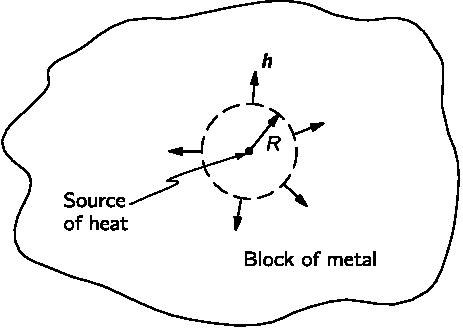
\includegraphics[width=0.6\linewidth]{fyz_fig0035.pdf}
          \caption{V oblasti blízko bodového zdroje proudí teplo radiálně směrem ven.}
          \label{fyz:fig0035}
        \end{figure}      
        Když je pole \(\vec{h}\) radiální a kulově symetrické, je integrál normálové složky vektoru
        \(\vec{h}\) kulovou plochou velmi jednoduchý, protože tehdy je normálová složka vektoru
        rovna velikosti vektoru \(\vec{h}\) a je konstantní. Obsah plochy, přes kterou integrujeme,
        je \(4\pi R^2\). Potom dostaneme 
        \begin{equation}\label{fyz:eq_gauss6}
          \oint_S\vec{h}\cdot\vec{n}\dd{S} = h\cdot4\pi R^2
        \end{equation}
        kde \(h\) je velikost vektoru \(\vec{h}\). Tento integrál má být roven \(P\), tedy rychlosti, 
        se kterou teplo ve zdroji vzniká. Dostáváme
        \begin{align}
          h       &= \frac{P}{4\pi R^2}                \nonumber                  \\
          \shortintertext{nebo}
          \vec{h} &= \frac{P}{4\pi R^2}\vec{e_r}       \label{fyz:eq_gauss7}
        \end{align} 
        kde, jako obvykle, \(\vec{e_r}\) představuje jednotkový vektor v radiálním směru. Podle 
        našeho výsledku je \(\vec{h}\) přímo úměrné \(P\) a mění se nepřímo úměrně s druhou mocninou 
        vzdálenosti od zdroje.
        
        Výsledek, který jsme právě dostali, se hodí na proudění tepla v blízkosti bodového zdroje
        tepla. Pokusme se nyní najít rovnice pro nejobecnější případ proudění tepla, platí-li jediná
        podmínka, že teplo se zachovává. Budeme se zabývat pouze tím, co se stane v prostoru bez
        jakýchkoliv zdrojů nebo absorbátorů tepla.
        
        Diferenciální rovnice pro vedení tepla byla odvozena v kapitole 
        \ref{fyz:IIchapII}. Podle rovnice (\ref{fyz:eq685}) platí
        \begin{equation}\label{fyz:eq_gauss8}
        \vec{h}=-\lambda\nabla T
        \end{equation}    
        (vzpomeňte si, že tento vztah platí sice přibližně, ale pro takové látky jako jsou kovy,
        docela dobře.) Dá se použít, samozřejmě, jen v těch oblastech látky, ve kterých nedochází ke
        generování nebo absorpci tepla. Už jsme odvodili jiný vztah, rovnici (\ref{fyz:eq_gauss4}),
        který platí, když se teplo zachovává. Když v (\ref{fyz:eq_gauss4}) vektor \(\vec{h}\)
        vyjádříme podle (\ref{fyz:eq_gauss8}), dostaneme
        \begin{align}
          - \der{q}{t} &= \nabla\cdot\vec{h} = - \nabla\cdot(\lambda\nabla T)     \nonumber    \\ 
          \intertext{nebo}
            \der{q}{t} &= \lambda\nabla\cdot\nabla T = \lambda\nabla^2 T     \label{fyz:eq_gauss9}
        \end{align}
        je-li \(\lambda\) konstanta. Vzpomínáte si, že \(q\) je množství tepla v jednotkovém objemu a
        \(\nabla\cdot\nabla = \nabla^2\) je \emph{Laplaceův operátor}
        \begin{equation*}
          \nabla^2= \pder{ }{x^2} + \pder{ }{y^2} + \pder{ }{z^2}.
        \end{equation*}       
      
        Uděláme-li ještě jeden předpoklad, můžeme dostat velmi zajímavou rovnici. Budeme 
        předpokládat, že teplota látky je přímo úměrná tepelnému obsahu jednotkového objemu, tj. že 
        látka má určitou  měrnou tepelnou kapacitu. Platí-li tento předpoklad (což bývá často), 
        můžeme psát
        \begin{align}
          \Delta q   &= c_V\Delta T                                        \nonumber    \\ 
          \intertext{nebo}
          \der{q}{t} &= c_V\der{T}{t}.                                     \label{fyz:eq_gauss10}
        \end{align}    
        Rychlost změny tepla je přímo úměrná rychlosti změny teploty. Součinitel úměrnosti \(c_V\)
        je \emph{měrná tepelná kapacita jednotky objemu látky}. Ze vztahů (\ref{fyz:eq_gauss10}) a
        (\ref{fyz:eq_gauss9}) dostáváme
        \begin{equation}\label{fyz:eq_gauss11}
          \der{T}{t} = \frac{\lambda}{c_V}\nabla^2T
        \end{equation}
        Zjišťujme, že časová rychlost změny \(T\) v každém bodě je přímo úměrná Laplaceovu operátoru 
        teploty \(T\), tj. druhé derivaci její závislosti na poloze v prostoru. Dostáváme 
        diferenciální rovnici s proměnnými \(x\), \(y\), \(z\) a \(t\) pro teplotu \(T\).
        
        Diferenciální rovnice (\ref{fyz:eq_gauss11}) se nazývá \emph{rovnicí difúze tepla}. Často je 
        psána ve tvaru
        \begin{equation}\label{fyz:eq_gauss12}
          \der{T}{t} = D\nabla^2T
        \end{equation}
        kde \(D\) je koeficient \emph{difúze} tepla a zde je roven hodnotě
        \(\displaystyle\frac{\lambda}{c_V}\).
        
        Rovnice difúze se objevuje v mnoha fyzikálních úlohách - při difúzi plynů, neutronů a v
        dalších případech. Nyní však máme úplnou rovnici, která popisuje difúzi v nejobecnější možné
        situaci. Později probereme způsoby řešení rovnice difúze, abychom našli, jak se v
        konkrétních případech mění teplota. Nyní se vrátíme zpět k výkladu dalších vět o vektorových
        polích.
  
    %------------- Cirkulace vektorového pole ------------------------------------------------------- 
    \subsection{Cirkulace vektorového pole}\label{fyz:IIchapIIIsecIV}

      Podobným způsobem, jakým jsme to udělali v případě divergence, chceme nyní prozkoumat rotaci. 
      Gaussovu větu jsme odvodili analýzou plošného integrálu, ačkoli zpočátku nebylo zřejmé, že se 
      chystáme zabývat divergencí. Jak jsme věděli, že máme integrovat přes celou plochu, abychom 
      dostali divergenci? Vůbec nebylo jasné, že vyjde tento výsledek. A právě bez zjevného  
      opodstatnění teď vypočítáme pomocí vektoru ještě cosi a ukážeme, že to souvisí z rotací. 
      Tentokrát budeme počítat to, co se nazývá cirkulace vektorového pole. Je-li \(\vec{C}\) nějaké 
      vektorové pole, vezmeme jeho složku podél nějaké křivky a vypočítáme integrál této složky po 
      celé uzavřené křivce. Tento integrál se nazývá cirkulací vektorového pole po (uzavřené) křivce. 
      Už dříve v této kapitole jsme uvažovali křivkový integrál vektoru \(\nabla\Psi\). Nyní 
      provedeme totéž pro jakékoliv vektorové pole \(\vec{C}\).
      
      Nechť je \(\Gamma\) nějaká uzavřená křivka v prostoru - pouze myšlená (obr. \ref{fyz:fig0201a}). 
      Křivkový integrál tangenciální složky vektoru \(\vec{C}\) po této křivce bude
      \begin{equation}\label{fyz:eq_fey_circ1}
        \oint_\Gamma C_t\dd{s} = \oint_\Gamma\vec{C}\cdot\dd{\vec{s}}.
      \end{equation}    
      
      Je nutné si všimnout, že se integruje po celé křivce kolem dokola, nejen z jednoho bodu do 
      druhého, jako jsme to dělali předtím. To, že je třeba integrovat po celé dráze dokola, má 
      připomenout malý kroužek na znaku integrování. Tento integrál se nazývá \emph{cirkulace 
      vektorového pole po křivce} \(\Gamma\). Název se převzal ze zkoumání cirkulace kapaliny a 
      podobně jako tok se rozšířil a použil na jakékoliv pole, i když tam není žádná „cirkulující“ 
      látka.
      
      Stejnou hrou, jakou jsme předvedli v případě toku, můžeme ukázat, že cirkulace po křivce je 
      součtem cirkulací po dvou dílčích křivkách. Předpokládejme, že jsme naši křivku na obr. 
      \ref{fyz:fig0201a} rozdělili na dvě uzavřené křivky spojením dvou bodů \((1)\) a \((2)\) na 
      původní křivce nějakou čarou napříč (obr. \ref{fyz:fig0201b}). Nyní existují dvě uzavřené 
      křivky  a \(\Gamma_1\) a \(\Gamma_2\). \(\Gamma_1\) je vytvořena z \(\Gamma_a\)-té části 
      původní křivky, která je vlevo od \((1)\) a (2) plus zkratka \(\Gamma_{ab}\). Křivku 
      \(\Gamma_2\) vytváří zbytek původní křivky plus zkratka.
      
      \begin{figure}[ht!]
        \centering
        \subcaptionbox{\label{fyz:fig0201a}}{\luafigure[0.45]{fyz_fig0201a.pdf}}   
        \subcaptionbox{\label{fyz:fig0201b}}{\luafigure[0.45]{fyz_fig0201b.pdf}}    
        \caption{Cirkulace vektorového pole \(C\): a) Cirkulace vektorového pole \(\vec{C}\) po 
                  křivce \(\Gamma\) je křivkový integrál \(\vec{C}\) ( tj. tangenciální složky vektoru 
                  \(\vec{C}\); b) Cirkulace po celé křivce \(\Gamma_a+\Gamma_b\) je rovna součtu 
                  cirkulací po dvou křivkách:\(\Gamma_1=\Gamma_a+\Gamma_{ab}\) a \(\Gamma_2=\Gamma_b
                  +\Gamma_{ab}\).}
        \label{fyz:fig0201}
      \end{figure} 
    
      Cirkulace po \(\Gamma_1\), je součtem integrálů po \(\Gamma_a\) a po \(\Gamma_{ab}\). Podobně 
      cirkulace po \(\Gamma_2\) je součtem dvou částí, jedné související s \(\Gamma_a\) a druhé 
      související s \(\Gamma_{ab}\). Integrál po \(\Gamma_{ab}\) bude mít v případě křivky 
      \(\Gamma_2\) opačné znaménko než v případě \(\Gamma_1\), protože směr oběhu bude opačný - vždyť 
      oba naše křivkové integrály musíme počítat ve stejném smyslu oběhu.
          
      Toutéž úvahou, jakou jsme provedli dříve, se můžeme přesvědčit, že součet obou těchto cirkulací
      dá právě křivkový integrál po původní křivce \(\Gamma\). Příspěvky pocházející od 
      \(\Gamma_{ab}\) se ruší. Cirkulace po jedné částí plus cirkulace po druhé částí je rovna 
      cirkulaci po vnější křivce. S procesem rozdělování původní křivky můžeme pokračovat do 
      jakéhokoliv počtu menších uzavřených drah. Sečteme-li cirkulace po menších dráhách, dojdeme 
      vždy k rušení příspěvků od jejich společných částí, takže součet je ekvivalentní s cirkulací po 
      původní křivce.       
  
      \begin{figure}[ht!]  %\ref{fyz:fig0038}
        \centering
        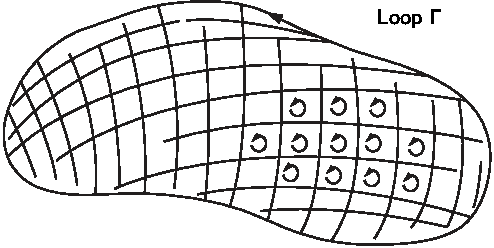
\includegraphics[width=0.7\linewidth]{fyz_fig0038.pdf}
        \caption{Je zvolena nějaká plocha ohraničená uzavřenou křivkou \(\Gamma\). Plocha se rozdělí  
                  na množství malých přibližně čtvercových plošek. Cirkulace po \(\Gamma\) je rovna 
                  sumě cirkulací po malých uzavřených křivkách.}
        \label{fyz:fig0038} 
      \end{figure}
      Nyní předpokládejme, že původní uzavřená křivka ohraničuje nějakou plochu. Ve skutečnosti
      existuje nekonečně mnoho ploch, jež všechny mají původní křivku jako svoji hranici. Naše
      výsledky však nebudou záviset na tom, kterou plochu zvolíme. Nejdříve rozdělíme naši původní
      křivku na mnoho malých uzavřených křivek, jež všechny budou ležet na námi zvolené ploše, jak
      je vidět na obr. \ref{fyz:fig0038}. Zvolíme-li naše křivky dostatečně malé, můžeme, bez ohledu
      na tvar plochy, předpokládat, že každá z nich utváří v podstatě rovinnou plošku. Kromě toho
      můžeme křivky vybrat tak, že každá bude velmi blízká obvodu čtverce. Cirkulaci po velké křivce
      nyní můžeme vypočítat tak, že najdeme cirkulace po obvodech všech malých čtverců a ty sečteme.   
        
    %------------- CIRKULACE PO OBVODU ČTVERCE. STOKESOVA VĚTA ---------------------------------------
    \subsection{Cirkulace po obvodu čtverce. Stokesova věta}\hypertarget{fyz:IIchapIIIsecV}
      Jak najít cirkulaci pro každý z malých čtverečků? Závisí to na tom, jak je čtvereček 
      orientovaný v prostoru. Kdyby měl speciální orientaci, například kdyby ležel v některé ze 
      souřadnicových rovin, bylo by možné výpočet provést snadno. Protože jsme dosud o orientaci 
      souřadnicových os neudělali žádný předpoklad, můžeme si osy dobře zvolit tak, aby ten 
      čtvereček, na který je v té chvíli soustředěna naše pozornost, ležel v rovině \(xy\) (obr. 
      \ref{fyz:fig0039}).
      
      Vyjádříme-li náš výsledek ve vektorové symbolice, můžeme tvrdit, že bude pro všechny konkrétní 
      orientace roviny tentýž.
  
      Nyní chceme najít cirkulaci pole \(\vec{C}\) po obvodu našeho malého čtverce. Křivkový
      integrál se snadno vypočte, uděláme-li čtvereček tak malý, že podél jakékoliv jeho strany se
      vektor \(\vec{C}\) moc nemění. (Tento předpoklad platí tím lépe, čím menší je čtvereček, takže
      v podstatě mluvíme o infinitezimálních čtverečcích.) Vyjdeme z bodu \((x, y)\) - levého
      dolního rohu obrázku - a budeme postupovat ve směru vyznačeném šipkami. V případě první
      strany, označené 1, nechť je tangenciální složka \(C_x(1)\), délka dráhy nechť je \(\Delta
      x\). První příspěvek k integrálu tedy bude \(C_x(1)\Delta x\). V případě druhé strany
      dostaneme \(C_y(2)\Delta y\), v případě třetí \(-C_x(3)\Delta x\) a v případě čtvrté strany to
      bude \(-C_y(3)\Delta y\). Záporná znaménka jsou nutná, neboť tangenciální složku musíme
      vyjadřovat vzhledem ke směru postupu po obvodu. Celý křivkový integrál pak bude
      \begin{equation}\label{fyz:eq_fey_circ2}
        \oint\vec{C}\dd{\vec{s}} = C_x(1)\Delta x + C_y(2)\Delta y 
                                  - C_x(3)\Delta x - C_y(3)\Delta y.
      \end{equation}      
  
      Všimněme si prvního a třetího členu na pravé straně. Spolu dávají
      \begin{equation}\label{fyz:eq_fey_circ3}
        [C_x(1) - C_x(3)]\Delta x.  
      \end{equation}
      Mohli byste se domnívat, že podle naší aproximace je rozdíl v hranaté závorce roven nule. Je
      to tak, ale pouze v nulovém přiblížení. Můžeme však být přesnější a vzít v úvahu i rychlost
      změny \(\vec{C_x}\). Když to uděláme, můžeme psát
      \begin{equation}\label{fyz:eq_fey_circ4}
        C_x(3) = C_x(1)+\pder{C_x}{y}\dd{y}.  
      \end{equation}
      Kdybychom zahrnuli následující přiblížení, vystoupily by v něm i členy obsahující \(\Delta
      y^2\). Protože však nakonec přejdeme k limitě pro \(\Delta y\rightarrow0\), je možno takové 
      členy zanedbat. Dosadíme-li (\ref{fyz:eq_fey_circ4}) do (\ref{fyz:eq_fey_circ3}), jistíme, že
      \begin{equation}\label{fyz:eq_fey_circ5}
        [C_x(1) - C_x(3)]\Delta x = -\pder{C_x}{y}\dd{x}\dd{y}.  
      \end{equation}  
      Souhlasně s naší aproximací je možno tuto derivaci počítat v bodě \((x, y)\).             
  
      \begin{figure}[ht!]  %\ref{fyz:fig0039}
        \centering
        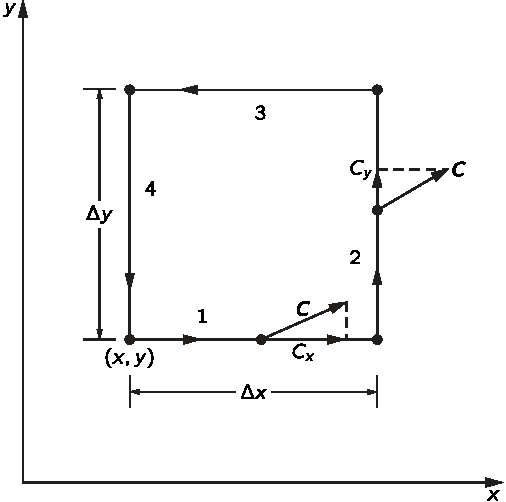
\includegraphics[width=0.7\linewidth]{fyz_fig0039.pdf}
        \caption{Výpočet cirkulace \(\vec{C}\) po obvodu malého čtverečku}
        \label{fyz:fig0039}
      \end{figure}
      Podobně můžeme vyjádřit zbývající dva členy ve výrazu (\ref{fyz:eq_fey_circ2}) pro cirkulaci
      \begin{equation}\label{fyz:eq_fey_circ6}
        [C_y(2) - C_y(4)]\Delta y = \pder{C_y}{x}\dd{x}\dd{y}.  
      \end{equation}    
      Cirkulace po obvodu čtverečku pak bude
      \begin{equation}\label{fyz:eq_fey_circ7}
        \left(\pder{C_y}{x}-\pder{C_x}{y}\right)\dd{x}\dd{y}.  
      \end{equation}    
      což je zajímavé, neboť rozdíl závorkách představuje právě \(z\)-ovou složku rotace. Kromě toho
      si všimněme, že \(\Delta x\Delta y\) je plošný obsah našeho čtverečku. Takovýmto způsobem
      můžeme naši cirkulaci (\ref{fyz:eq_fey_circ7}) psát jako
      \begin{equation}\label{fyz:eq_fey_circ8}
        (\nabla\times\vec{C})_z\dd{S}.  
      \end{equation}
      Ale \(z\)-ová složka ve skutečnosti znamená normálovou složku vzhledem k plošnému elementu. 
      Cirkulaci po obvodu diferenciálního čtverečku proto můžeme vyjádřit v invariantním vektorovém 
      tvaru:
      \begin{equation}\label{fyz:eq_fey_circ9}
        \oint\vec{C}\cdot\dd{\vec{s}} 
          = (\nabla\times\vec{C})_n\Delta S = (\nabla\times\vec{C})\cdot\vec{n}\Delta S.  
      \end{equation} 
      Náš výsledek zní: cirkulace jakéhokoliv vektoru \(\vec{C}\) po obvodu infinitezimálního 
      čtverečku je rovna normálové (vzhledem k rovině, v níž leží čtvereček) složce vektoru 
      \(\rot{C}\) vynásobené plošným obsahem čtverečku.
    
      Cirkulaci po jakékoliv uzavřené křivce \(\Gamma\) je možné nyní lehce uvést do souvislosti s 
      rotací vektorového pole. Křivku „vyplníme“ nějakou vhodnou plochou \(S\) (obr. 
      \ref{fyz:fig0036}) a vypočítáme cirkulace po obvodech množiny infinitezimálních čtverečků 
      tvořících tuto plochu. Tento součet je možno zapsat jako integrál. Naším výsledkem je velmi 
      užitečná věta, nazvaná Stokesova věta (podle G. G. Stokese).
    
      \begin{flalign}
        \text{\textbf{Stokesova věta}:}                                              && 
        \oint_\Gamma\vec{C}\cdot\dd{\vec{s}} = \int_S(\nabla\times\vec{C})_n\dd{S}.  &&
      \end{flalign}
      kde \(S\) je jakákoliv plocha ohraničená křivkou \(\Gamma\). 
  
      \begin{figure}[ht!]  %\ref{fyz:fig0036}
        \centering
        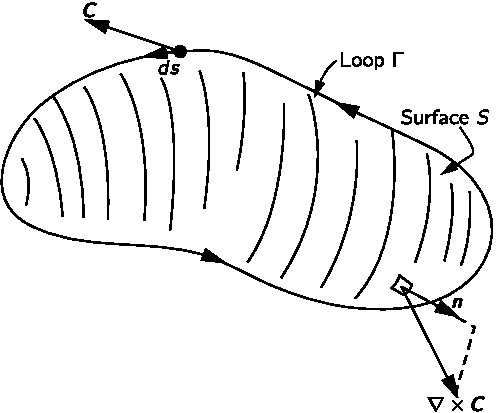
\includegraphics[width=0.7\linewidth]{fyz_fig0036.pdf}
        \caption{Cirkulace \(\vec{C}\) po \(\Gamma\) je rovna plošnému integrálu normálové složky
          vektoru \(\nabla\times\vec{C}\)}
        \label{fyz:fig0036}   
      \end{figure} 
      Nyní musíme něco říci o znaménkové konvenci. Na obr. \ref{fyz:fig0039} směřuje osa 
      \(z\) ke čtenáři v „obyčejné“, tj. pravotočivé soustavě. Kdybychom náš křivkový integrál 
      počítali při kladné orientaci oběhu, zjistili bychom, že cirkulace je rovna \(z\)-ové složce 
      vektoru \(\nabla\times\vec{C}\). Kdybychom postupovali opačným směrem, dostali bychom opačné 
      znaménko. Jak tedy budeme obecně vědět, který směr zvolit za kladný pro normálovou složku 
      vektoru \(\nabla\times\vec{C}\)? Kladná normála musí souviset se smyslem rotace vždy tak, jak 
      je to na obr. \ref{fyz:fig0039}. Obecný případ je vyznačen na obr. \ref{fyz:fig0036}.
  
      Jedním ze způsobů, jak si tento vztah zapamatovat, je \emph{pravidlo pravé ruky}. Přiložíte-li
      \emph{pravou} ruku podél křivky \(\Gamma\) tak, že prsty ukazují kladný smysl
      \(\dd{\vec{s}}\), palec ukazuje směr kladné normály k ploše \(S\).
  
  
    %------------- POLE S NULOVOU ROTACÍ A DIVERGENCÍ ------------------------------------------------
    \subsection{Pole s nulovou rotací a divergencí}\label{fyz:IIchapIIIsecVI}
      Nyní bychom se rádi zabývali některými důsledky našich nových vět. Nejdřív vezměme příklad 
      vektoru, jehož rotace je všude rovna nule. Pak je podle Stokesovy věty jeho cirkulace po každé 
      křivce také rovna nule. Z toho vyplývá, že zvolíme-li na uzavřené křivce dva body \((1)\) a 
      \((2)\) (obr. \ref{fyz:fig0043}), \emph{křivkový integrál tangenciální složky z \((1)\) do 
      \((2)\) nezávisí na tom, po které ze dvou možných drah se vypočítá.} Můžeme udělat závěr, že 
      integrál z \((1)\) do \((2)\) bude záviset pouze na poloze těchto bodů, tj. je pouze nějakou 
      funkcí polohy. Stejnou logiku jsme použili v kapitole \ref{vol02:fyz:IchapXIII}, kde jsme 
      dokázali, že když je integrál nějaké veličiny po uzavřené dráze vždy roven nule, lze jej 
      vyjádřit jako rozdíl funkce polohy dvou bodů. Tento fakt nám umožnil zavést pojem 
      \textbf{potenciálu}. Dále jsme dokázali, že \emph{vektorové pole je gradientem této 
      potenciálové funkce} (viz vztah \ref{vol02:fyz:eq008}).
  
      \begin{figure}[ht!]  %\ref{fyz:fig0043}
        \centering
        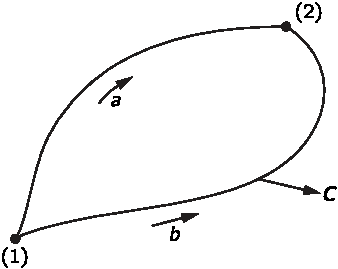
\includegraphics[width=0.6\linewidth]{fyz_fig0043.pdf}
        \caption{Je-li \(\nabla\times\vec{C}\) rovno nule, cirkulace po uzavřené křivce \(\Gamma\)   
          je také rovna nule. Křivkový integrál \(\vec{C}\cdot\dd{\vec{s}}\) z (1) do (2) po 
          křivce \(a\) proto musí být stejný jako tentýž křivkový integrál po křivce \(b\).}
        \label{fyz:fig0043}
      \end{figure}
      Z toho vyplývá, že každé vektorové pole s nulovou rotací je rovno gradientu nějaké skalární 
      funkce. To je užitečný poznatek: je-li \(\nabla\times\vec{C}=0\), existuje skalární pole 
      \(\Psi\) (psí), že \(\vec{C}=\nabla\Psi\). Tento zvláštní druh vektorového pole tedy můžeme, 
      chceme-li, popsat pomocí skalárního pole.
      
      Ukážeme ještě něco. Předpokládejme, že máme \emph{libovolné} skalární pole \(\varphi\) (fí). 
      Vytvoříme-li jeho gradient \(\nabla\varphi\), musí být integrál tohoto vektoru po jakékoliv 
      uzavřené křivce  roven nule. Jeho křivkový integrál z bodu \(1\) do bodu \(2\) bude 
      \(\varphi(2) - \varphi(1)\). Představují-li \(1\) a \(2\) tentýž bod, bude podle věty 1 (vztah 
      \ref{fyz:eq273}) křivkový integrál roven nule:
      \begin{equation}\label{fyz:eq359}
        \limitint_{\mathclap{\substack{\text{jakákoliv}\\\text{uzavřená}\\\text{křivka}}}}
          \nabla\varphi\dd{\vec{s}} = 0
      \end{equation}
      Na základě Stokesovy věty můžeme udělat závěř, že 
      \begin{equation}\label{fyz:eq_fey_null0} 
        \int(\nabla\times(\nabla\varphi))_n\dd{S} = 0
      \end{equation} 
      pro \emph{jakoukoliv plochu}. Je-li tento integrál roven nule pro každou plochu, musí být 
      roven nule i jeho integrand. Vždy tedy platí
      \begin{equation}
        \nabla\times(\nabla\varphi) = 0
      \end{equation}
      Tentýž výsledek jsme dokázali v článku \ref{fyz:IIchapIIsecVII} pomocí vektorové algebry.      
      
          
      Nyní se podívejme na zvláštní případ, kdy malou uzavřenou křivku \(\Gamma\) vyplníme velkou 
      plochou \(S\), jako na obr. \ref{fyz:fig0037}. Rádi bychom se vlastně dozvěděli, co se 
      stane, když se uzavřená křivka „scvrkne“ na bod, takže ohraničení plochy zmizí, tj. plocha se 
      stane uzavřenou. Je-li vektor \(\vec{C}\) všude konečný, musí se při „scvrkávání“ křivky 
      \(\Gamma\) křivkový integrál po \(\Gamma\) blížit nule (integrál je přibližně přímo úměrný 
      délce \(\Gamma\) která se blíží nule). Podle Stokesovy věty se musí plošný integrál veličiny 
      \((\nabla\times\vec{C})_n\) také blížit nule. Když plochu uzavíráme, jako bychom přidávali 
      příspěvky, které postupně vyruší to, co bylo předtím. Dospěli jsme k nové větě
      \begin{equation}\label{fyz:eq_fey_null1} 
        \limitoint_{\mathclap{\substack{\text{jakákoliv}\\\text{uzavřená}\\\text{křivka}}}}
          (\nabla\times\vec{C})_n \dd{s} = 0
      \end{equation}
  
      \begin{figure}[ht!]  %\ref{fyz:fig0037}
        \centering
        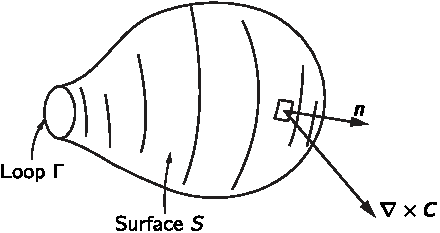
\includegraphics[width=0.7\linewidth]{fyz_fig0037.pdf}
        \caption{Přechodem k limitnímu případu uzavřené plochy zjistíme, že plošný integrál veličiny
                  \((\nabla\times\vec{C})_n\) musí konvergovat k nulové hodnotě.
                  \cite[s.~60]{Feynman02}}
        \label{fyz:fig0037}
      \end{figure}
      Nyní je to zajímavé, neboť jednu větu o plošném integrálu uzavřenou plochou už máme. Takový 
      plošný integrál je podle Gaussovy věty (vztah \ref{fyz:eq_gauss_veta}) roven objemovému 
      integrálu divergence vektorového pole. Z Gaussovy věty použité na vektor 
      \(\nabla\times\vec{C}\) vyplývá
      \begin{equation}\label{fyz:eq_fey_null2} 
        \limitint_{\mathclap{\substack{\text{uzavřená}\\\text{plocha}}}}
          (\nabla\times\vec{C})_n \dd{\vec{S}}
        =
        \limitint_{\mathclap{\substack{\text{objem uvnitř}\\\text{plochy}}}}
          \nabla\cdot(\nabla\times\vec{C})\dd{V}.
      \end{equation}
      Z toho usuzujeme, že druhý integrál musí být též roven nule:
      \begin{equation}\label{fyz:eq_fey_null3} 
        \limitint_{\mathclap{\substack{\text{jakýkoliv}\\\text{objem}}}}
        \nabla\cdot(\nabla\times\vec{C})\dd{V} = 0
      \end{equation}
              
      To také platí pro každé vektorové pole \(\vec{C}\). Protože však rovnost 
      (\ref{fyz:eq_fey_null3}) je správná pro \emph{každý objem}, musí platit, že v každém bodě 
      prostoru je integrand roven nule. Dostáváme, že vždy
      \begin{equation}\label{fyz:eq_fey_null4}
        \nabla\cdot(\nabla\times\vec{C})=0.
      \end{equation}
      To je však stejný výsledek, jaký jsme dostali v článku \ref{fyz:IIchapIIsecVII} z vektorové 
      algebry. Nyní začínáme chápat, jak jedno souvisí s druhým.      
    
    %---------------------- Shrnutí ------------------------------------------------------------------
    \subsection{Shrnutí}
      Shrňme, co jsme se dozvěděli o vektorovém počtu. Skutečně významné výsledky kapitol
      \ref{fyz:IIchapII} a \ref{fyz:IIchapIII} jsou tyto:
      \begin{enumerate}[noitemsep]
        \item Operátory \(\pder{ }{x}\), \(\pder{ }{y}\) a  \(\pder{ }{z}\) možno považovat za tři
              složky vektorového operátoru:
              \begin{equation}
                  \nabla = \left(\pder{ }{x}, \pder{ }{y}, \pder{ }{z}\right)
              \end{equation}
              Zachází-li se s tímto operátorem jako s vektorem, vzorce, které pro něj vyplývají z
              vektorové algebry, jsou správné.
        \item Rozdíl hodnot skalárního pole ve dvou bodech je roven křivkovému integrálu
              tangenciální složky gradientu tohoto skaláru po jakékoliv křivce spojující oba body:
              \begin{equation}
                \Psi(2)-\Psi(1) = 
                  \limitint_{\mathclap{\substack{(1)\\\text{jakákoli}\\\text{křivka}}}}^{(2)}
                  \nabla\Psi\cdot\dd{\vec{s}}
              \end{equation}
        \item Plošný integrál normálové složky libovolného vektoru po uzavřené ploše je roven 
              integrálu divergence tohoto vektoru přes vnitřní objem ohraničený plochou:
              \begin{equation}
                \limitint_{\mathclap{\substack{\text{uzavřená}\\\text{plocha}}}}          
                            \vec{C}\cdot\vec{n}\dd{S} 
              = \limitint_{\mathclap{\substack{\text{objem}\\\text{uvnitř}\\\text{plochy}}}} 
                          (\nabla\cdot\vec{C})\dd{V}, 
              \end{equation}
        \item Křivkový integrál tangenciální složky libovolného vektoru po uzavřené křivce je roven
              plošnému integrálu normálové složky rotace tohoto vektoru po jakékoliv ploše, která je
              touto křivkou ohraničena:
              \begin{equation}
                \limitint_{\mathclap{\substack{\text{hranice}}}}  
                  \vec{C}\cdot\dd{\vec{s}} =
                \limitint_{\mathclap{\substack{\text{plocha}}}}
                  (\nabla\times\vec{C})\cdot\vec{n}\dd{S}.
              \end{equation}            
      \end{enumerate}
        
    %------------- Vizualizace vektorového pole s využitím šumové textury ----------------------------
    \subsection{Vizualizace vektorového pole s využitím šumové textury}
      Záměrem této „názorné exkurze“ do teorie pole je poskytnout náhled s využitím animací. 
      Zopakujme že, vektor je veličina, která určuje nejen velikost, ale i směr v prostoru. Vektory 
      tedy používáme k popisu fyzikálních veličin, jako je např. rychlost, hybnost, zrychlení nebo 
      síla působící na objekt. Nicméně, pokud se pokoušíme popsat systém, který se skládá z velkého 
      počtu objektů (např. pohybující se voda, sníh, déšť,…), musíme přiřadit vektor každému 
      samostatnému objektu. Například v každém okamžiku můžeme jakékoliv sněhové vločce přiřadit 
      vektor rychlosti, který charakterizuje její pohyb. Padající sníh je příkladem diskrétního, tj. 
      nespojitého prostředí.    
      
      Stejné je to u analýzy pohybu tekutiny. I v tomto případě musíme vektor rychlosti přiřadit v
      každém okamžiku každé částečce tekutiny. Takto budou vektory popisovat směr a velikost
      rychlosti v každém čase a v každém bodě prostoru. Soubor všech vektorů rychlosti nazveme
      \emph{vektorovým polem} rychlostí. Nyní je jasný podstatný rozdíl mezi vektorovým a skalárním
      polem tj., že vektorové obsahuje informaci jak o velikosti, tak i o směru veličiny v každém
      časovém okamžiku pro každý bod v prostoru, zatímco skalární pouze udává velikost dané veličiny
      v každém čase a v každém bodě prostoru. Příkladem spojitého prostředí je např. proudění
      vzduchu.
      
      Obecné vektorové pole \(\vec{F}(x, y, z)\) můžeme napsat ve tvaru:
      \begin{equation}
        \vec{F}(x,y,z) = F_x(x,y,z)\vec{i} + F_y(x,y,z)\vec{j} + F_z(x,y,z)\vec{k},
      \end{equation} 
      kde jednotlivé komponenty jsou \emph{skalární pole}. Pro ilustraci vlastností vektorových polí 
      použijeme tekutinové pole, protože vizualizace takovýchto typů vektorových polí jsou 
      nejjednodušší.  
      
      Zobrazení vektorových polí je provedeno pomocí šumové textury, která je lokálně korelována se
      směrem vektorového pole. Obdobné zobrazení lze přirozeným způsobem realizovat i
      experimentálně. Rozházíme-li semínka trávy v silném elektrickém poli, začnou se orientovat
      delší osou rovnoběžně se směrem silokřivek pole. Poskytnou nám tím hustý soubor vzorků
      zobrazujících směry a tedy i tvar pole. Platí tedy, že lokální směry polí jsou v souhlase se
      směry šumové textury diagramu. Šumová textura umí poskytnout mnoho informací o prostorové
      struktuře pole.
  
      \begin{figure}[ht!]
        \centering
        \AddVideo{160}{130}{vf_div}
        \caption{Proudové pole má zřídlo v počátku souřadnic a proudnice od něho směřují radiálně} 
        \label{fyz:fig0_fey_anim1}
      \end{figure}
  
      \begin{figure}[ht!]
        \centering 
        \AddVideo{160}{130}{vf_curl} 
        \caption{Proudové pole je vytvářeno pouze vírem; je bez zřídla, tekutina se pohybuje po 
                  kružnicích a nedochází ani ke vzniku, ani k zániku částic tekutiny} 
        \label{fyz:fig0_fey_anim2}
      \end{figure}
      
      První animace \ref{fyz:fig0_fey_anim1} znázorňuje \emph{divergující tok} tekutiny, šumovou 
      texturou, jejíž směr je v korelaci se směrem tohoto toku. Animace na obr. 
      \ref{fyz:fig0_fey_anim2} zobrazuje jinou třídu chování toku tekutiny  - \emph{cirkulaci, 
      víření}. Kapalina se pohybuje jednoduše v kruzích, nic zde nevzniká ani nezaniká (nemá zdroj 
      ani propad).   
  
      Na animaci \ref{fyz:fig0_fey_anim3} je zřídlo v blízkosti menší výpusti (propadu), zatímco 
      animace \ref{fyz:fig0_fey_anim4} znázorňuje dvě zřídla nestejné síly. Tekutinové pole může mít 
      více než jeden střed víření. 
  
      \begin{figure}[ht!]
        \centering
        \AddVideo{160}{130}{vf_divdiv1} 
        \caption{Proudové pole je složeno ze zřídla a z propadu (tzv. proudový dipól); v okolí 
                  zřídla a propadu směřují proudnice vždy od zřídla směrem k propadu}
        \label{fyz:fig0_fey_anim3}
      \end{figure}
  
      Na animaci \ref{fyz:fig0_fey_anim5} je ukázán tok pole se dvěma víry, cirkulacemi. Toky víří v
      opačných směrech a jeden je silnější než druhý. Na animaci \ref{fyz:fig0_fey_anim6} máme
      stejnou situaci, ale směry obou vírů jsou stejné.    
      
      Na animaci \ref{fyz:fig0_fey_anim7} je ukázán konstantní tok klesající dolů, který se vzájemně
      ovlivňuje se zřídlem. Zdroj je částečně schopen téci vzhůru proti proudu padající tekutiny,
      ale nakonec je také stržen a otočen směrem dolů.
      
      Podobně na animaci \ref{fyz:fig0_fey_anim8} je znázorněn homogenní tok směřující dolů,
      interagující s tokem cirkulujícím proti směru hodinových ručiček. Otáčivý tok je schopen téci
      kousek proti proudu, ale nakonec je stržen silnějším tokem směrem dolů.
  
      \begin{figure}[ht!]
        \centering
        \AddVideo{160}{130}{vf_divdiv2} 
        \caption{Proudového pole je v reálném čase deformováno ve směru rychlostního pole a je 
                  složeno ze dvou různě silných zřídel v různých místech; v blízkém okolí obou zřídel 
                  se proudnice pohybují směrem od zřídel}
        \label{fyz:fig0_fey_anim4}
      \end{figure} 
  
      \begin{figure}[ht!]
        \centering  
        \AddVideo{160}{130}{vf_curlcurl2}  
        \caption{Proudového pole je v reálném čase deformována ve směru rychlostního pole a je 
                  složeno ze dvou různě silných vírů v různých místech; směr rotace jednoho víru je ve 
                  směru hodinových ručiček a druhého proti směru hodinových ručiček}
        \label{fyz:fig0_fey_anim5}
      \end{figure} 
  
      \begin{figure}[ht!]
        \centering
        \AddVideo{160}{130}{vf_curlcurl1} 
        \caption{Proudového pole je v reálném čase deformována ve směru rychlostního pole a je  
                  složeno ze dvou různě silných vírů v různých místech; směr rotace obou vírů je v 
                  tomto případě shodný}
        \label{fyz:fig0_fey_anim6}
      \end{figure} 
      
      Konečně na animaci \ref{fyz:fig0_fey_anim9} jsou ukázány oba toky pole, jak vír, tak i zdroj
      (jak rotace, tak také divergence vektorového pole jsou nenulové). Jakékoli vektorové pole lze
      zapsat jako součet nevírových částí (nulová rotace) a nedivergujících (nezřídlových,
      nezdrojových) částí (žádná zřídla ani propady částic). V našem studiu elektromagnetizmu
      uvidíme, že\emph{ statické elektrické pole je nevírové} (tj. vypadá jako na animacích
      \ref{fyz:fig0_fey_anim1}, \ref{fyz:fig0_fey_anim3}, \ref{fyz:fig0_fey_anim4} a
      \ref{fyz:fig0_fey_anim7}) a \emph{statické magnetické pole je nedivergující, nezdrojové} (tj.
      podobá se animacím \ref{fyz:fig0_fey_anim2}, \ref{fyz:fig0_fey_anim5},
      \ref{fyz:fig0_fey_anim6} a \ref{fyz:fig0_fey_anim8}). Jenom v případech časově proměnného
      elektrického pole můžeme pozorovat, že má elektrické pole obě vlastnosti, tj. je jak zdrojové,
      tak i vírové, takže vypadá jako na animaci \ref{fyz:fig0_fey_anim9}. Narozdíl od pole
      elektrického je pole magnetické vždy nezdrojové (nedivergentní), a to i v časově proměnných
      situacích. To znamená, že magnetické pole se vždy podobá modelům z animacím
      \ref{fyz:fig0_fey_anim2}, \ref{fyz:fig0_fey_anim5}, \ref{fyz:fig0_fey_anim6} a
      \ref{fyz:fig0_fey_anim8}.              
      
      \begin{figure}[ht!]
        \centering
        \AddVideo{160}{130}{vf_divconstant}   
        \caption{Proudového pole je v reálném čase deformována ve směru  
                  rychlostního pole a je vytvářeno zřídlem umístěným v 
                  homogenním konstantním toku, který míří shora dolů 
                  (tzv. Rankinovo polotěleso, Rankinův ovál)}
        \label{fyz:fig0_fey_anim7}
      \end{figure}
  
      \begin{figure}[ht!]
        \centering
        \AddVideo{160}{130}{vf_curlconstant}    
        \caption{Proudového pole je v reálném čase deformována ve směru   
                  rychlostního pole a je složeno z víru a homogenního toku 
                  směřujícího shora dolů}
        \label{fyz:fig0_fey_anim8}
      \end{figure}
  
      \begin{figure}[ht!]
        \centering 
        \AddVideo{160}{130}{vf_divcurl}
        \caption{Proudového pole je v reálném čase deformována ve směru    
                  rychlostního pole a je vytvářeno kombinací víru a zřídla}
        \label{fyz:fig0_fey_anim9}
      \end{figure}
  
%~~~~~~~~~~~~~~~~~~~~~~~~~~~~~~~~~~~~~~~~~~~~~~~~~~~~~~~~~~~~~~~~~~~~~~~~~~~~~~~~~~~~~~~~~~~~~~~~~~